\chapter{Experiment} \label{cpt-experiment}

When considering occlusion culling algorithms that can be used in specific use cases, the runtime 
performance is a critical aspect. But runtime performance is a multi-dimensional measure, in that 
most algorithms provide certain results under specific circumstances and by setting several constraints, 
like a use in interiors only or the use of pre-calculated data. To be able to evaluate the strengths 
and weaknesses of this work's implementation, an in-depth experiment was conducted and evaluated, 
highlighting a diverse set of measured data. \\

\noindent
To conduct the experiment, the method of measuring performance was chosen because it allows for 
an in-depth analysis of the pipeline steps. When accurately measuring the two configurations, 
\ac{PONOC} and \ac{PMOC}, and comparing them to a baseline configuration without occlusion culling 
enabled, the difference between both can be evaluated by looking at the individual pipeline steps 
and their timings. A cross-comparison between pipelines using different models provides additional 
insights into why the computation times scale and how the complexity of the scene refers to the scaling. \\

\noindent
In the experiment, the two approaches, \ac{PONOC} and \ac{PMOC}, were evaluated in respect to 
culling efficiency, \ac{CPU} runtime performance, \ac{GPU} runtime performance, and pixel overdraw.
Additional measurements were performed using the base pipeline without occlusion culling to 
correctly evaluate the differences between both occlusion culling configurations. Furthermore, 
the computation of the best occluders was measured to evaluate a potential real-time alternation 
of the scene data. \\

\noindent
In this chapter, the experiment is first evaluated in how it shows the differences between the pipelines. 
In this context, various factors are discussed, and it is presented how these factors were taken into account 
during the experiment. After that, the tools that were used to perform the measurements are presented, as 
well as the models, which were tested. Finally, the results are discussed by presenting the measurements 
for each model. A summary of the most meaningful results is given in the end, aggregating average data from 
all the tests performed during the experiment.

\section{Experimental Setup} \label{sec-experimental-evaluation}

The experiment aimed to evaluate the tested scenes in respect to the above-mentioned aspects. To do this, 
various characteristics have been selected, which are outlined below. All aspects aim to demonstrate how 
the occlusion culling affected the given test scene, how the computations differed compared to the plain 
pipeline without any occlusion culling, and how it can be optimally used in practice.


\subsection*{Scenes} \label{subsec-models}

\begin{figure*}[!htb]
  \begin{subfigure}{80px}
      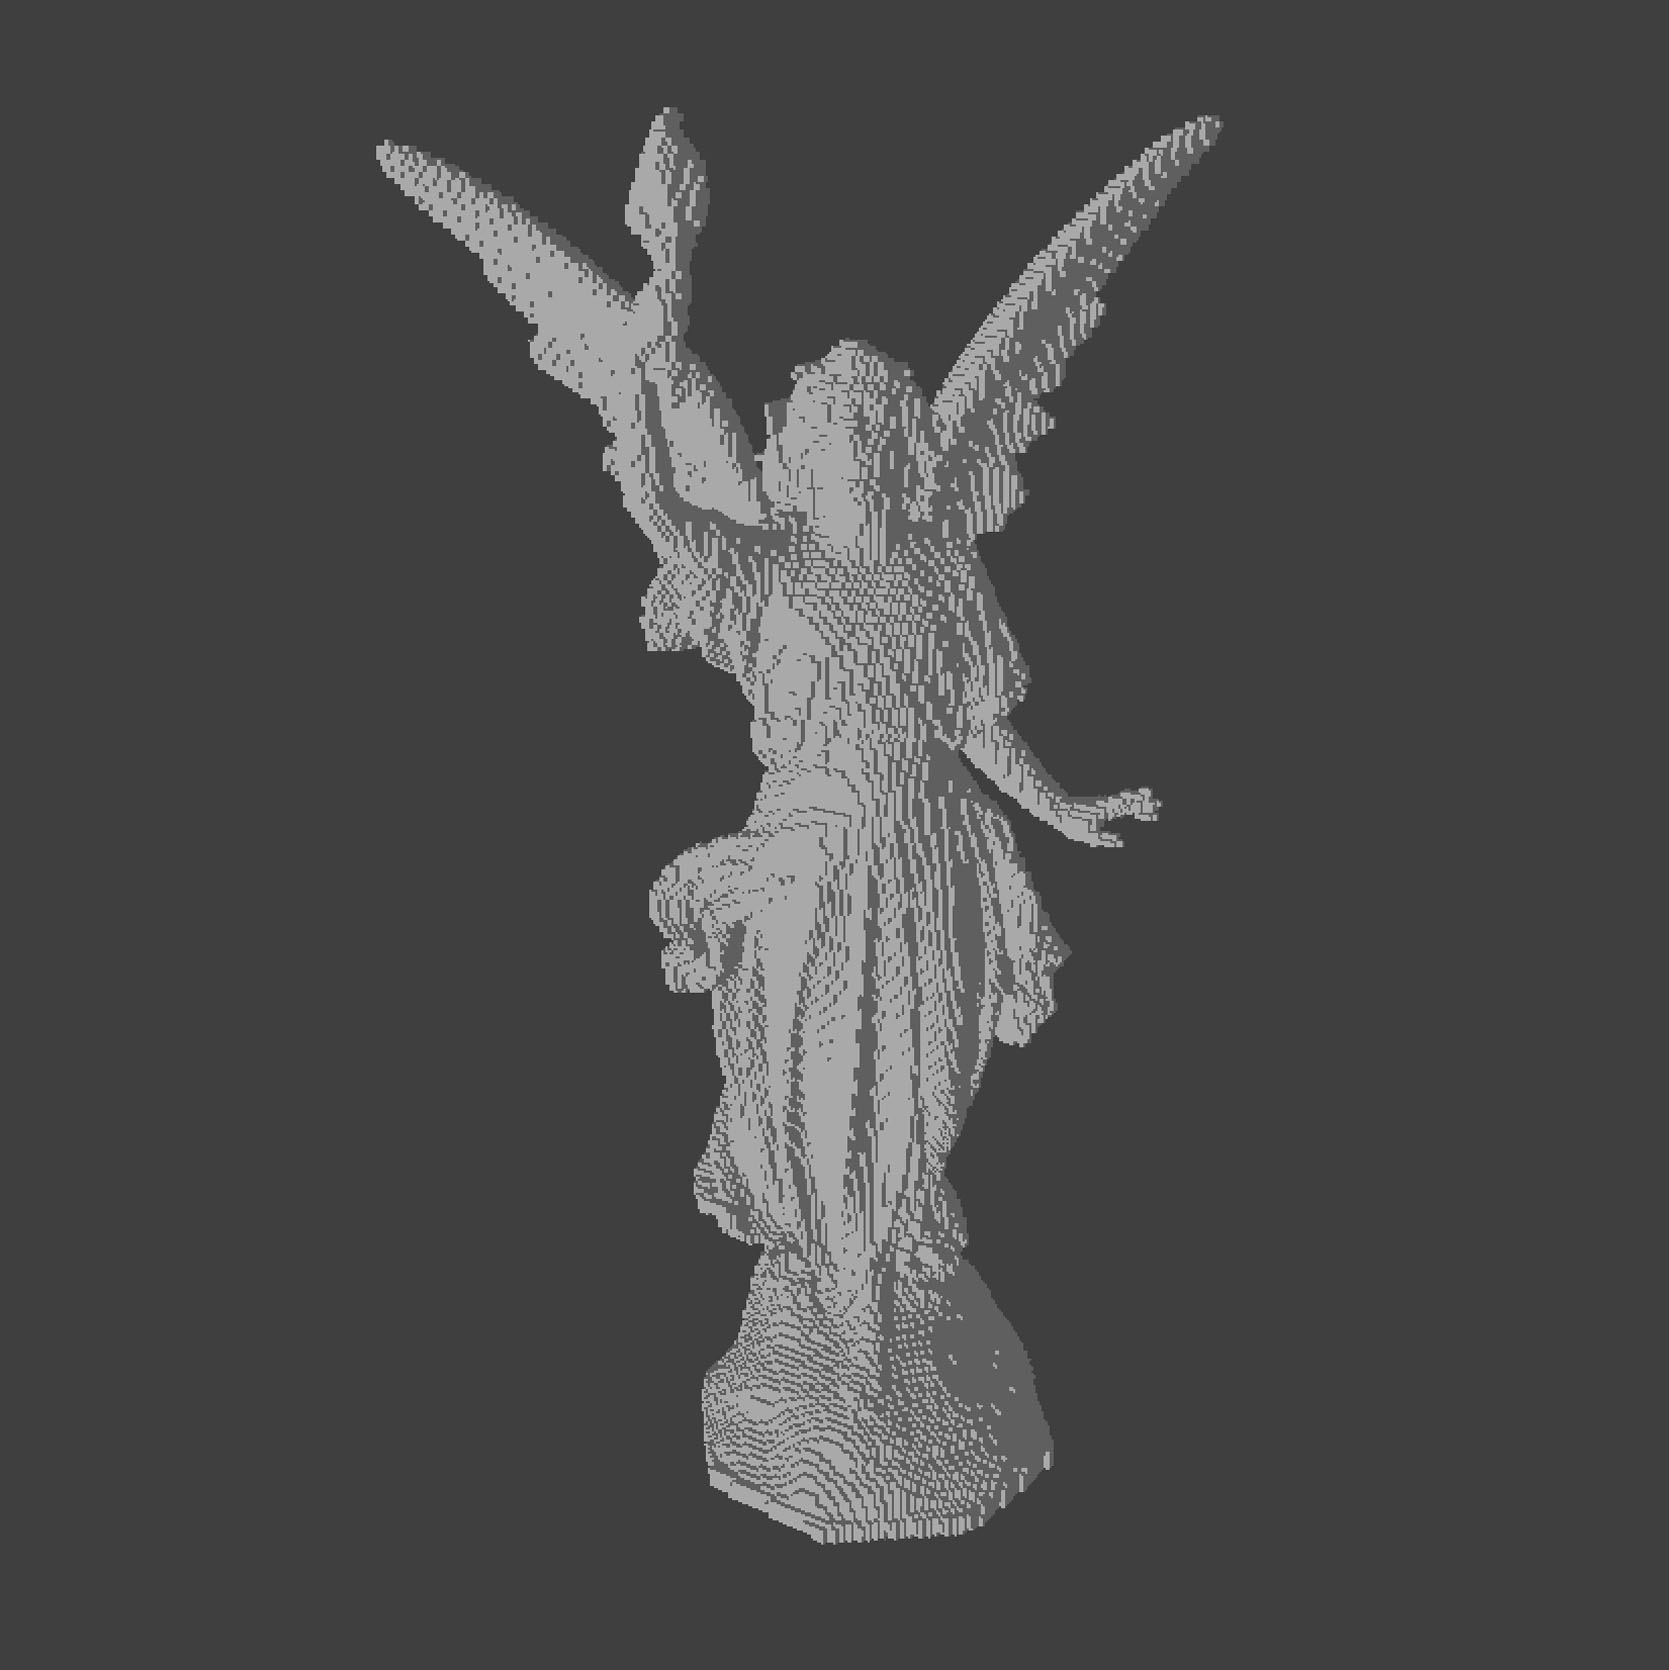
\includegraphics[width=80px]{images/graphics/model-lucy.jpg}
      \caption{Lucy}
      \parbox{\linewidth}{\centering\footnotesize 331,254 voxels,\\ 1600 best occluders}
  \end{subfigure}
  \begin{subfigure}{80px}
      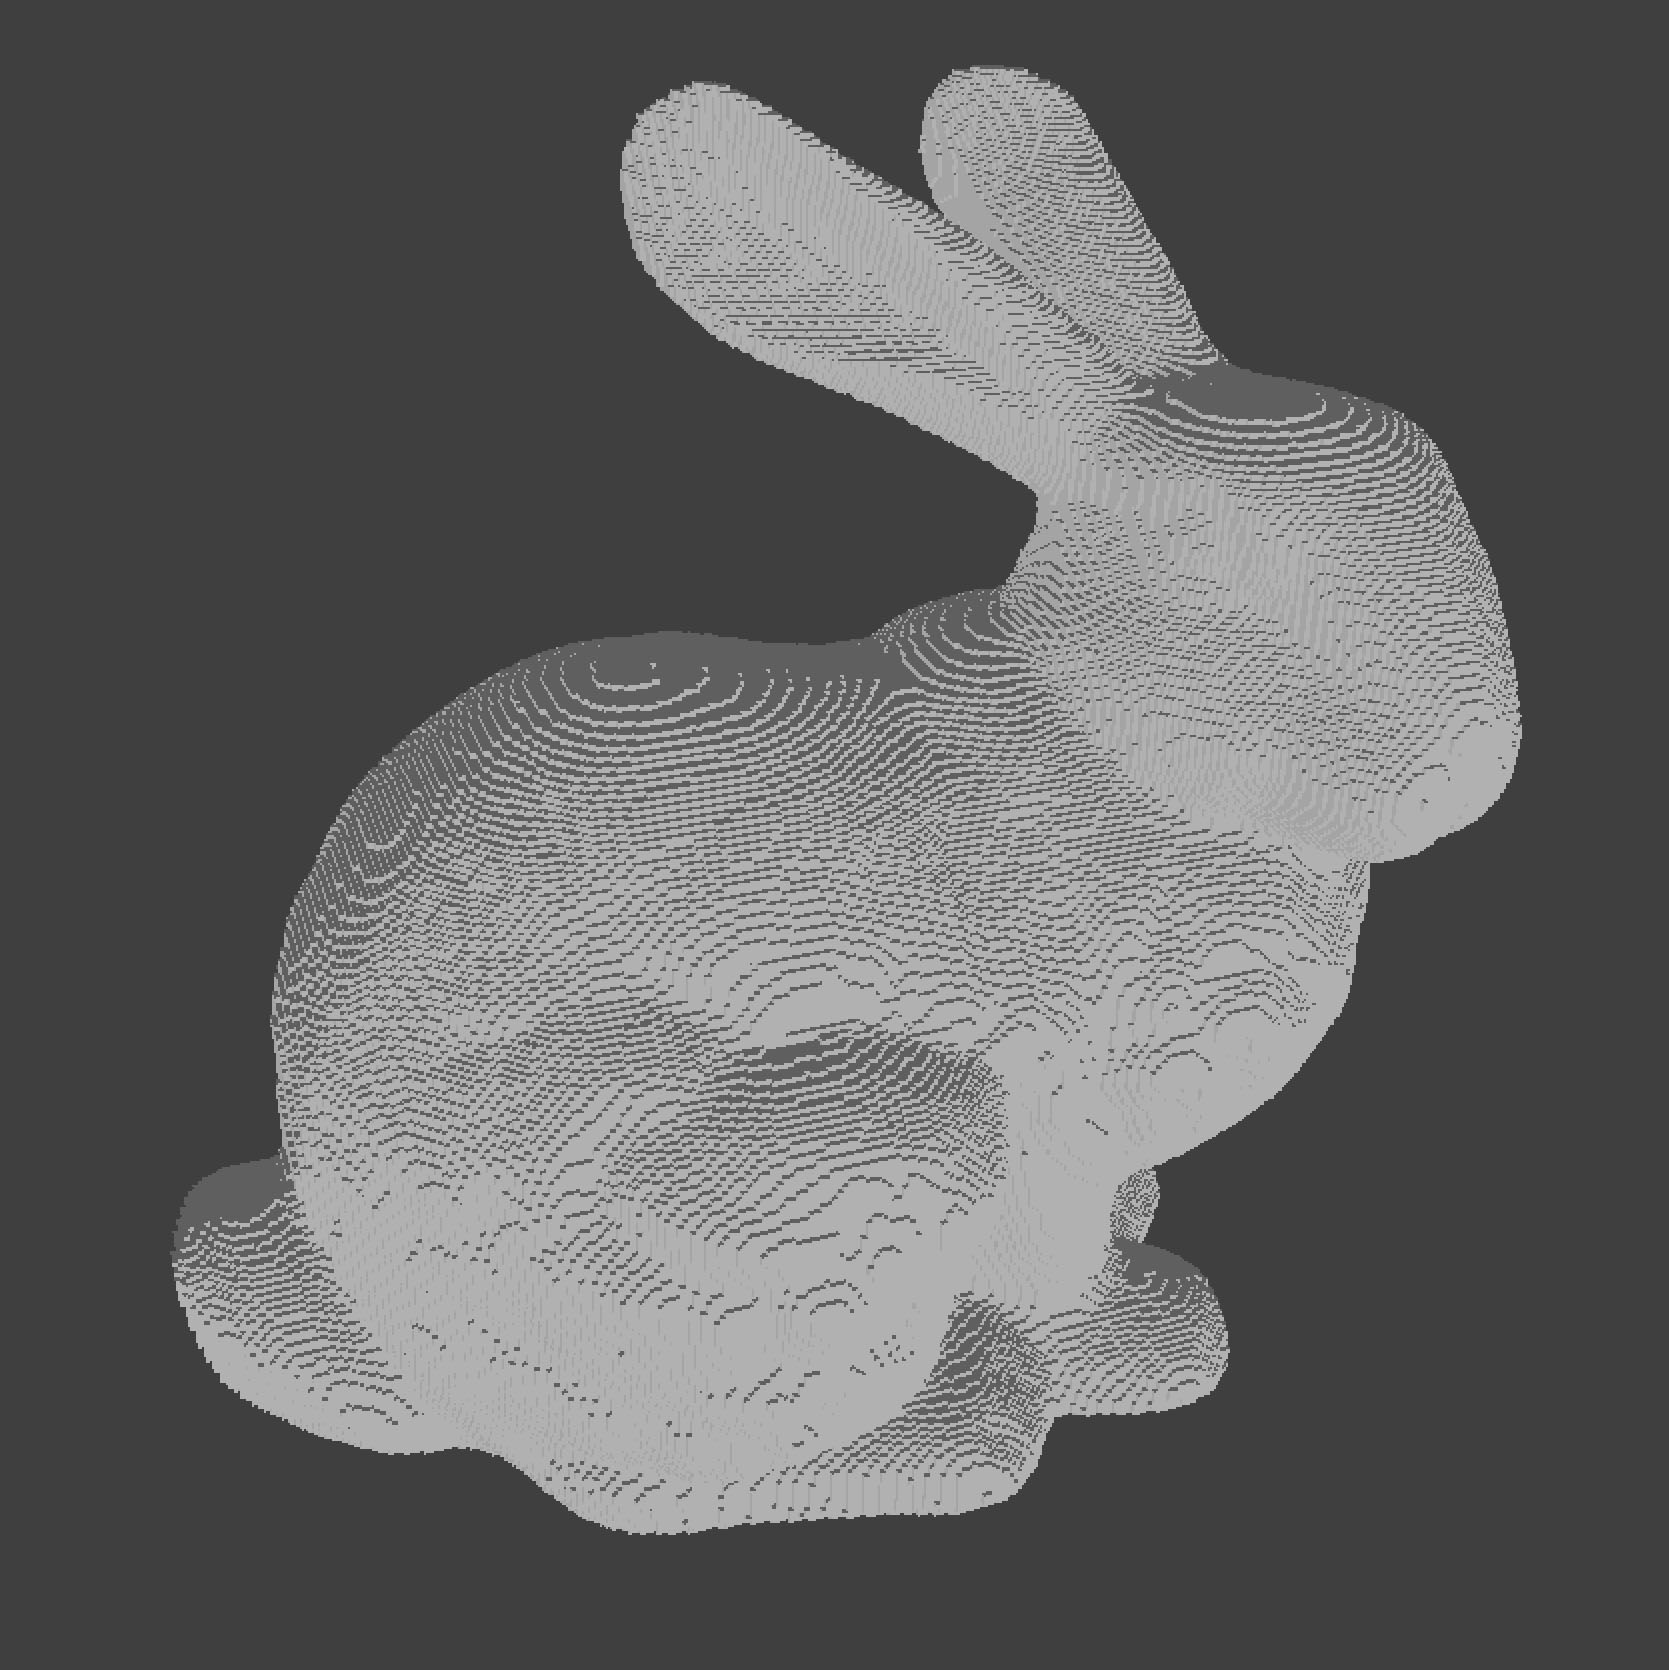
\includegraphics[width=80px]{images/graphics/model-bunny.jpg}
      \caption{Stanford Bunny}
      \parbox{\linewidth}{\centering\footnotesize 3,379,738 voxels,\\ 8256 best occluders}
  \end{subfigure}
  \begin{subfigure}{80px}
      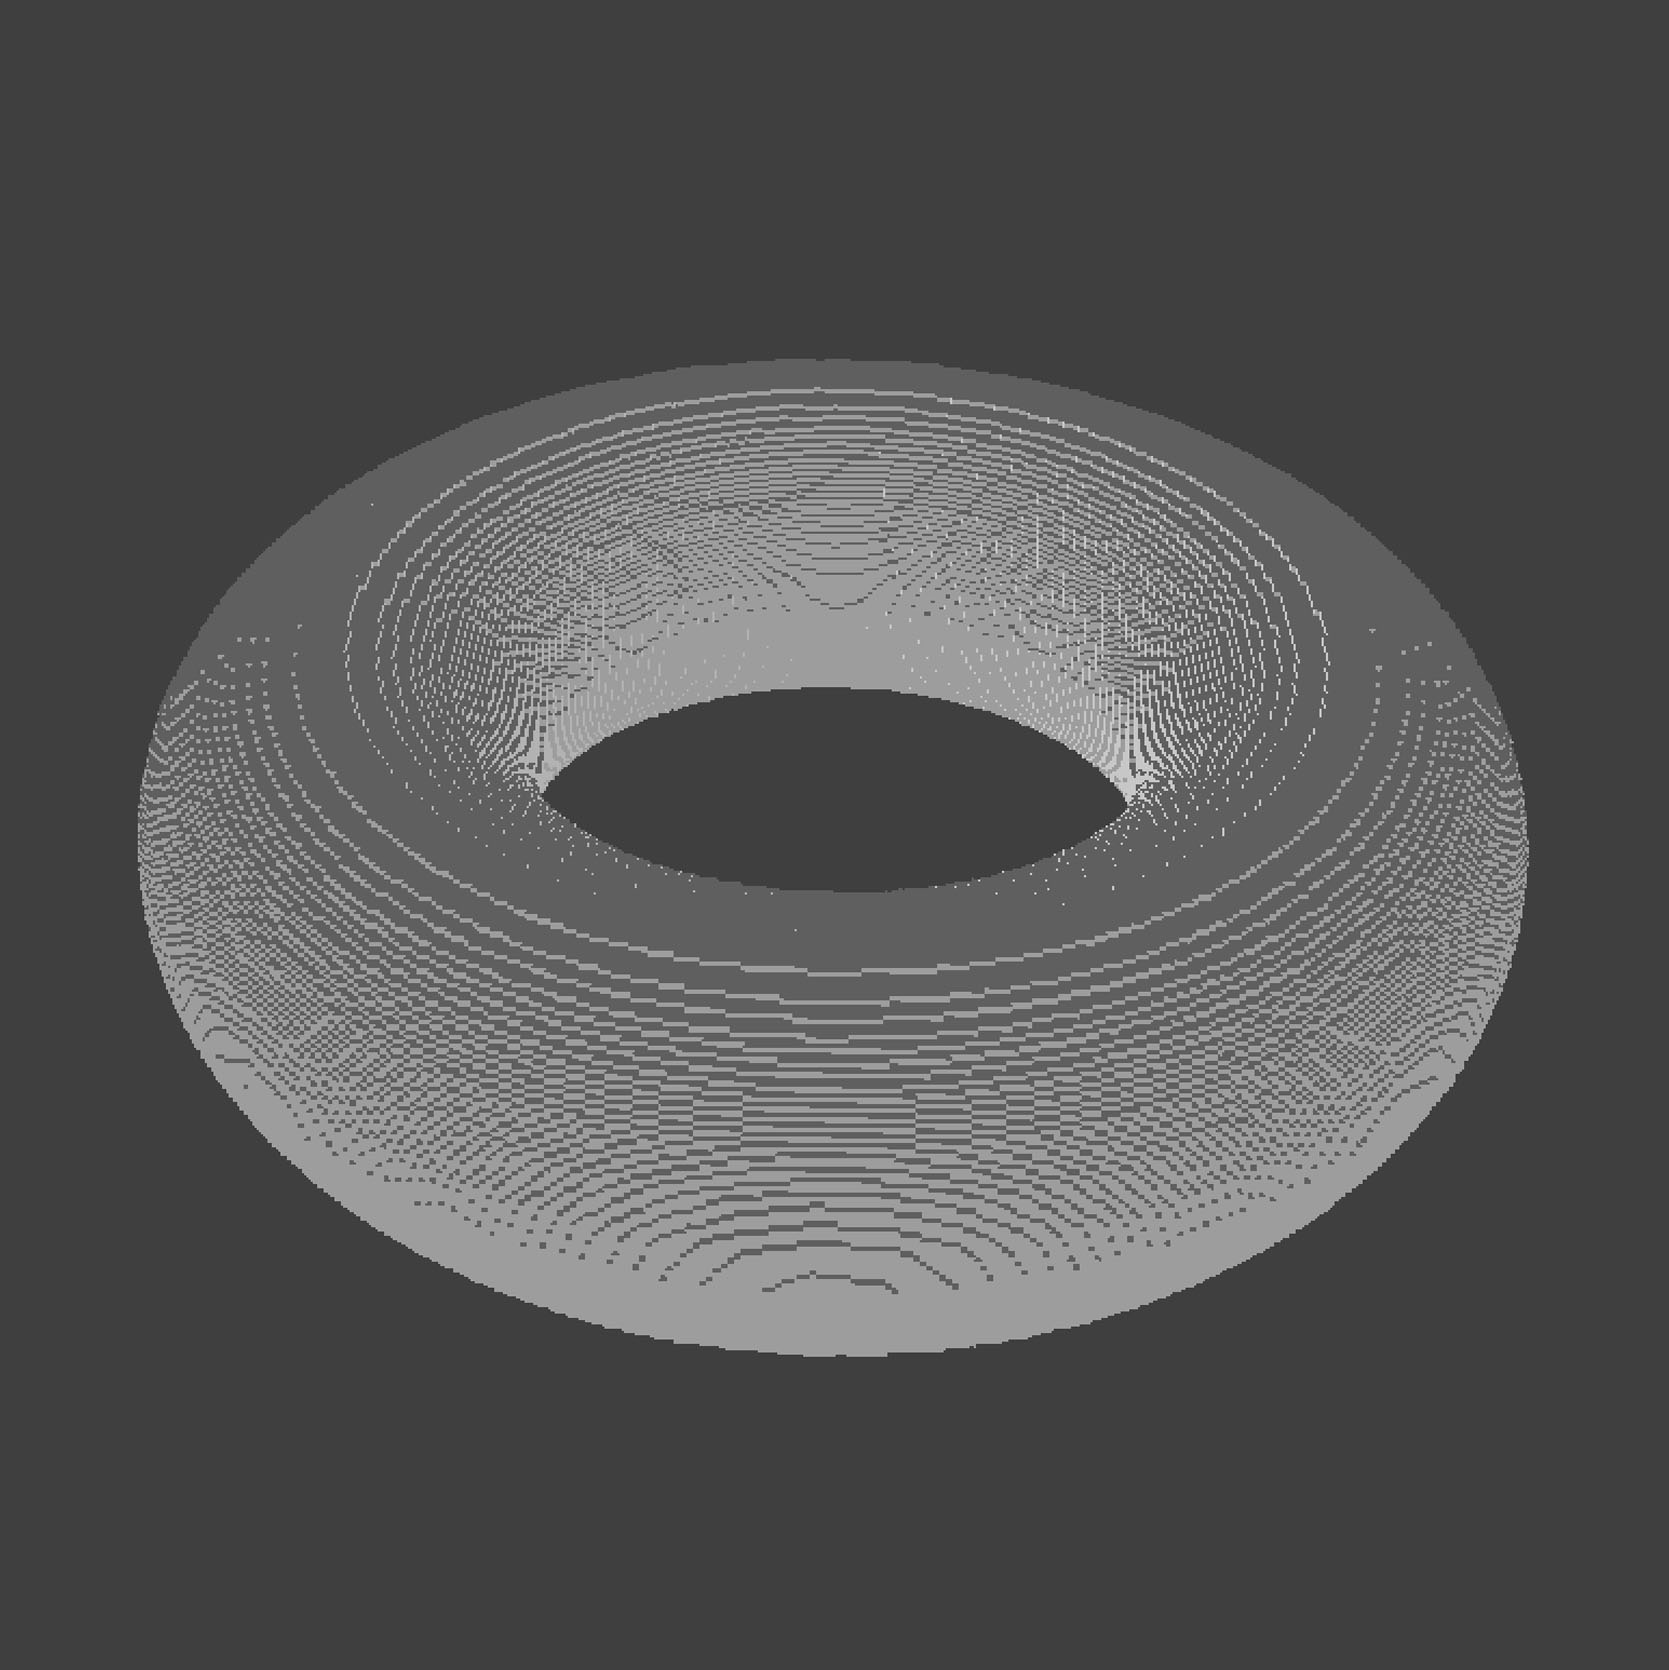
\includegraphics[width=80px]{images/graphics/model-torus.jpg}
      \caption{Torus}
      \parbox{\linewidth}{\centering\footnotesize 2,311,006 voxels,\\ 7168 best occluders}
  \end{subfigure}
  \begin{subfigure}{80px}
      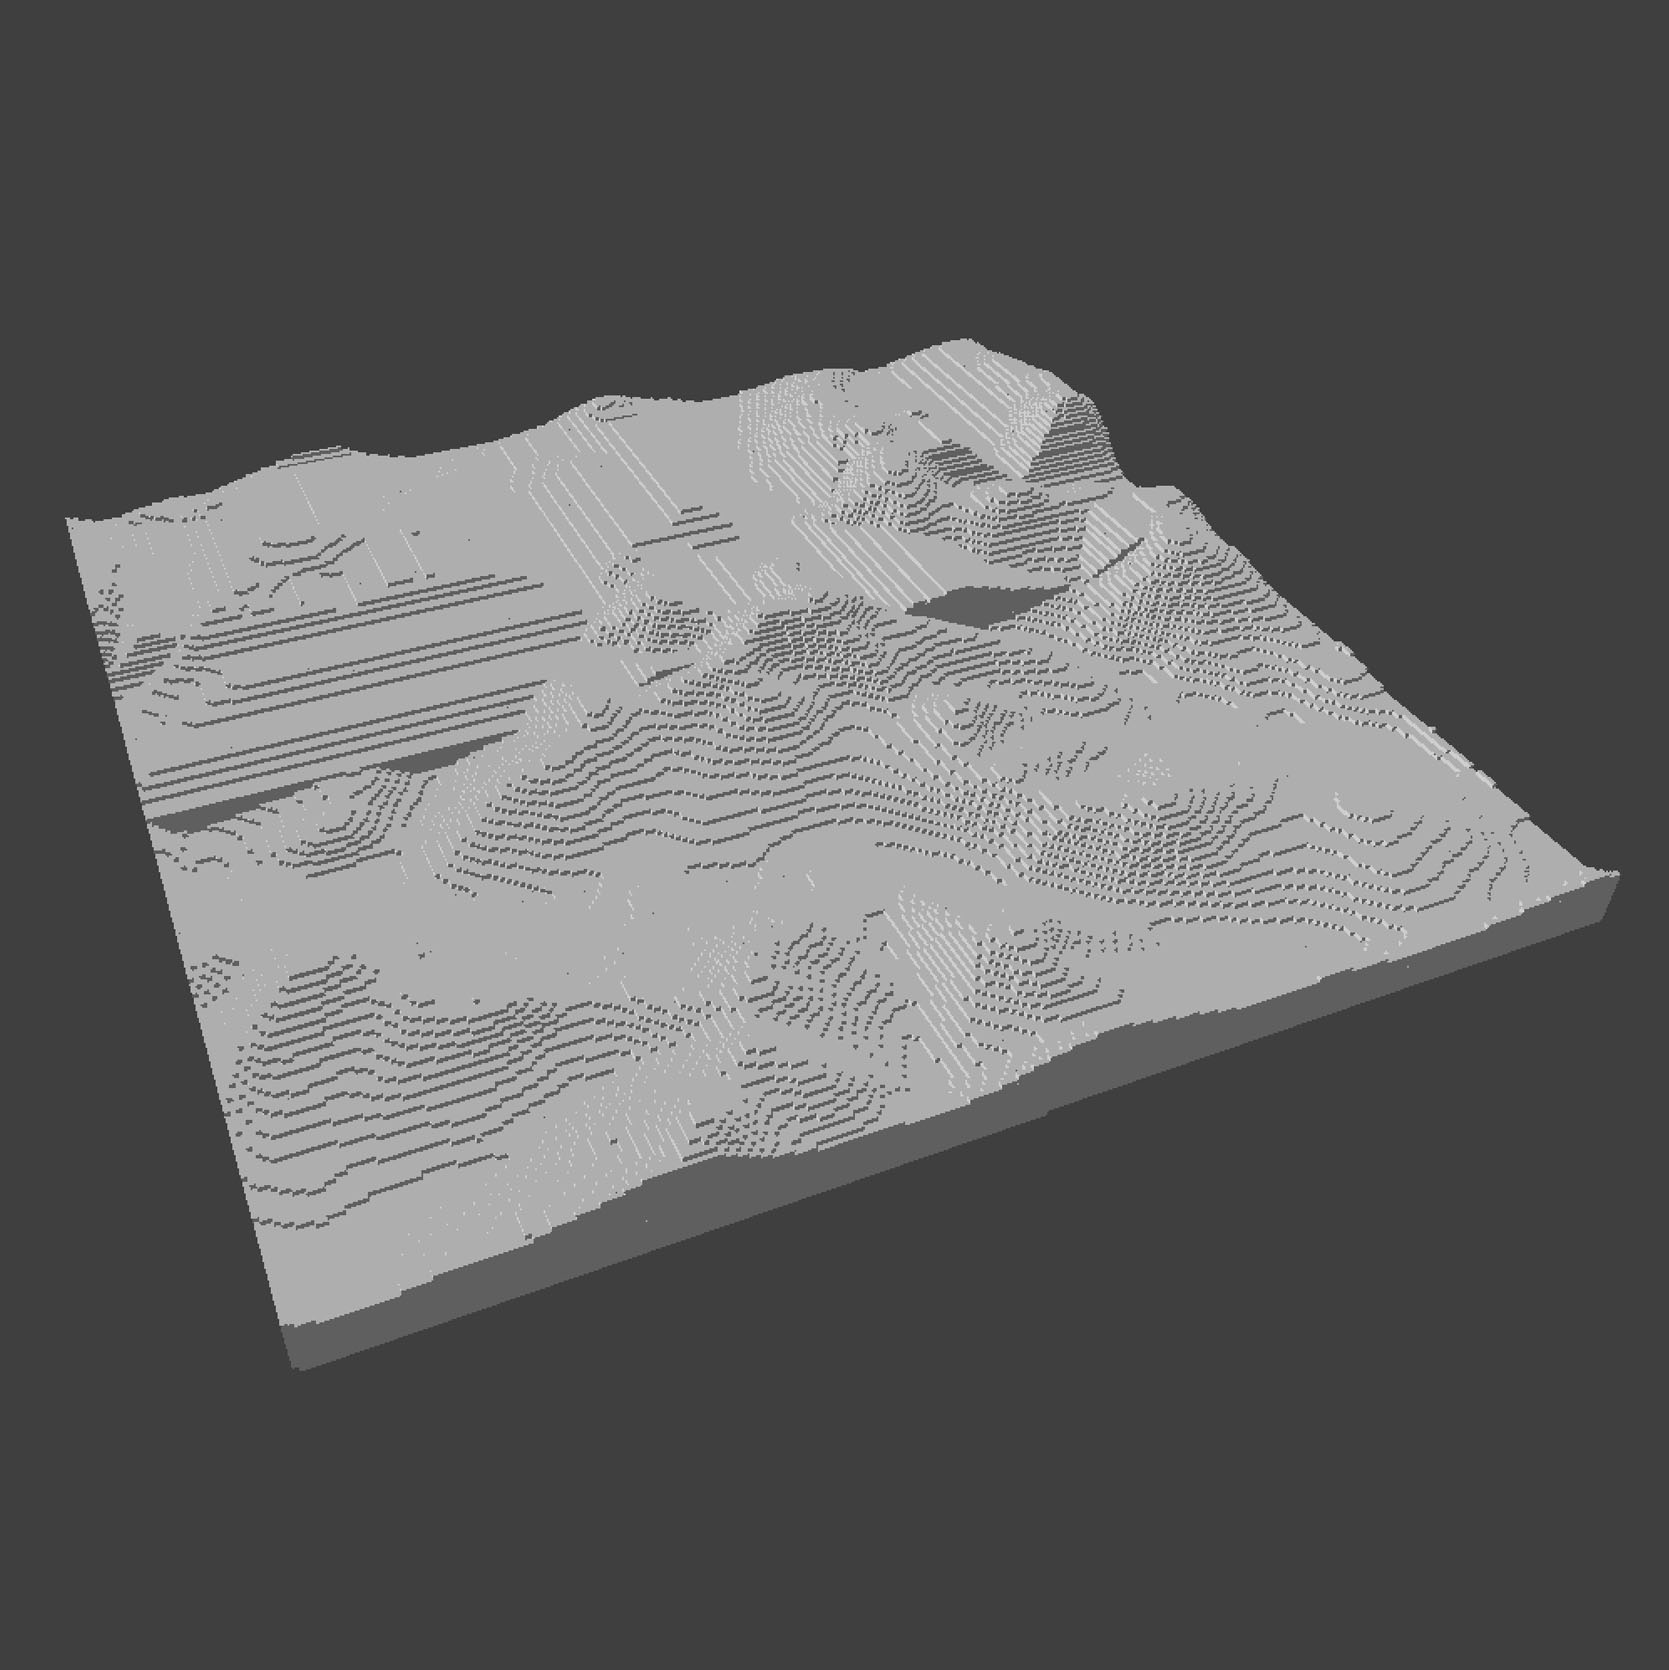
\includegraphics[width=80px]{images/graphics/model-terrain.jpg}
      \caption{Terrain}
      \parbox{\linewidth}{\centering\footnotesize 953,362 voxels,\\ 6976 best occluders}
  \end{subfigure}
  \begin{subfigure}{80px}
      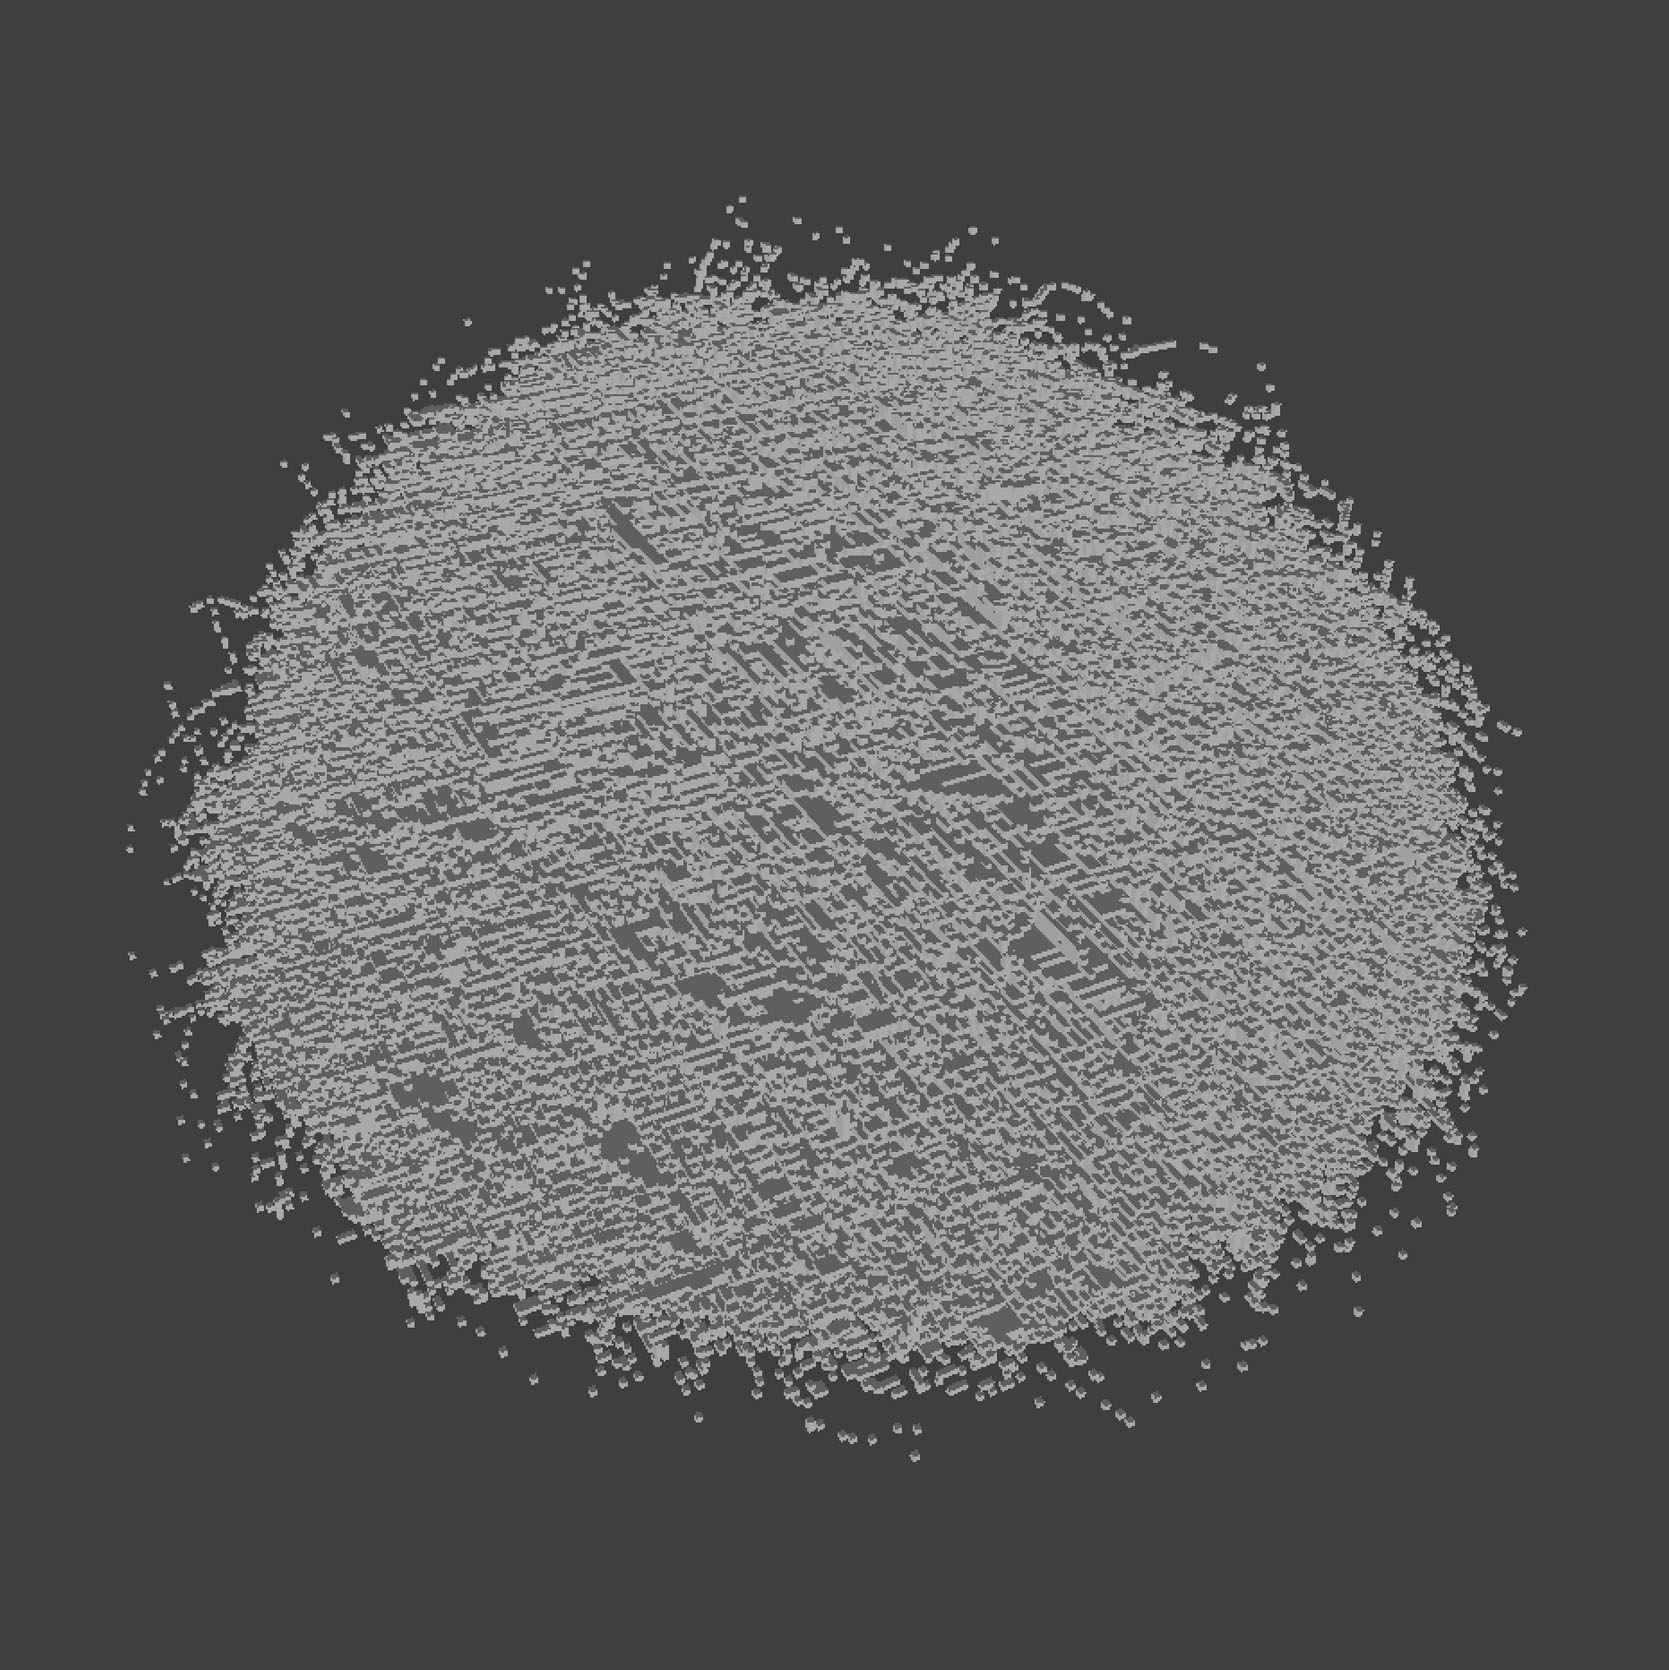
\includegraphics[width=80px]{images/graphics/model-hairball.jpg}
      \caption{Hairball}
      \parbox{\linewidth}{\centering\footnotesize 1,652,435 voxels,\\ 5056 best occluders}
  \end{subfigure}
  
  \caption{The scenes used for the experimental evaluation of the algorithm.}
  \label{fig:experiment-models}
\end{figure*}

\noindent
The scenes that were used in the tests are \emph{Lucy} (Stanford 3D Scanning Repository), the 
\emph{Stanford Bunny} (Stanford 3D Scanning Repository), the \emph{Hairball}, the \emph{Torus}, 
and a \emph{Terrain}. All of these scenes feature different characteristics, which tested 
the pipeline in a variety of ways. The models were voxelized to a size of $256^3$ and occupy 
different amounts of space within the scene. The scenes are listed in Figure 
\ref{fig:experiment-models}. \\

\begin{table}[htbp]
  \begin{center}
    \begin{tabular}{|c|c|c|c|}
      \hline
      \textbf{}&\multicolumn{3}{|c|}{\textbf{Scene Memory Footprint - $256^3$}} \\
      \cline{2-4} 
      \textbf{Scene} & \textbf{\textit{Voxel Data (KiB)}}& \textbf{\textit{Octree Node Buffer (KiB)}} & \textbf{\textit{Best Occluder Buffer (KiB)}} \\
      \hline
      Lucy        & 5,176   & 321   & 50  \\
      Bunny       & 52,808  & 2,697 & 258 \\
      Torus       & 36,109  & 1,866 & 224 \\
      Terrain     & 14,896  & 867   & 218 \\
      Hairball    & 25,819  & 1,857 & 158 \\
      \hline
    \end{tabular}
  \end{center}
  \caption{Memory footprint of the tested scenes.}
  \label{tbl:scene-data-size}
\end{table}

\noindent
Table \ref{tbl:scene-data-size} shows the memory footprint of the necessary data structures for 
each scene. Adding all three buffers together results in the total memory dedicated to the scene 
geometry.


\subsection*{Scene Layout} \label{subsec-scene-layout}

For the scene layout, the position of the model in the scene was important, and the data structure and 
topology were considered in particular. \\

\noindent
The data was sampled over time using a standardized camera animation, which was following a circular orbit 
around the scene, visualized in Figure \ref{fig:test-anim-camera-path}. A vertical offset was added to the orbit 
so the scene could be drawn from various angles. This was especially important for scenes like the \emph{Torus}, 
which are likely to behave very differently when viewed from above compared to when viewed from the side. \\

\noindent
Some of the scenes were filled up to the borders, others only occupied a small portion of the overall scene. 
Since the octree had always taken up the entire space of the scene, the overall scene layout was additionally 
challenged by different models. The \emph{Terrain} model, for example, only occupied the lower part of the 
scene but reached to each end of the sides, while the \emph{Lucy} model occupied only one quarter of the scene, 
reaching to the top end of the octree instead of the sides. \\

\begin{figure}[h]
    \centering
    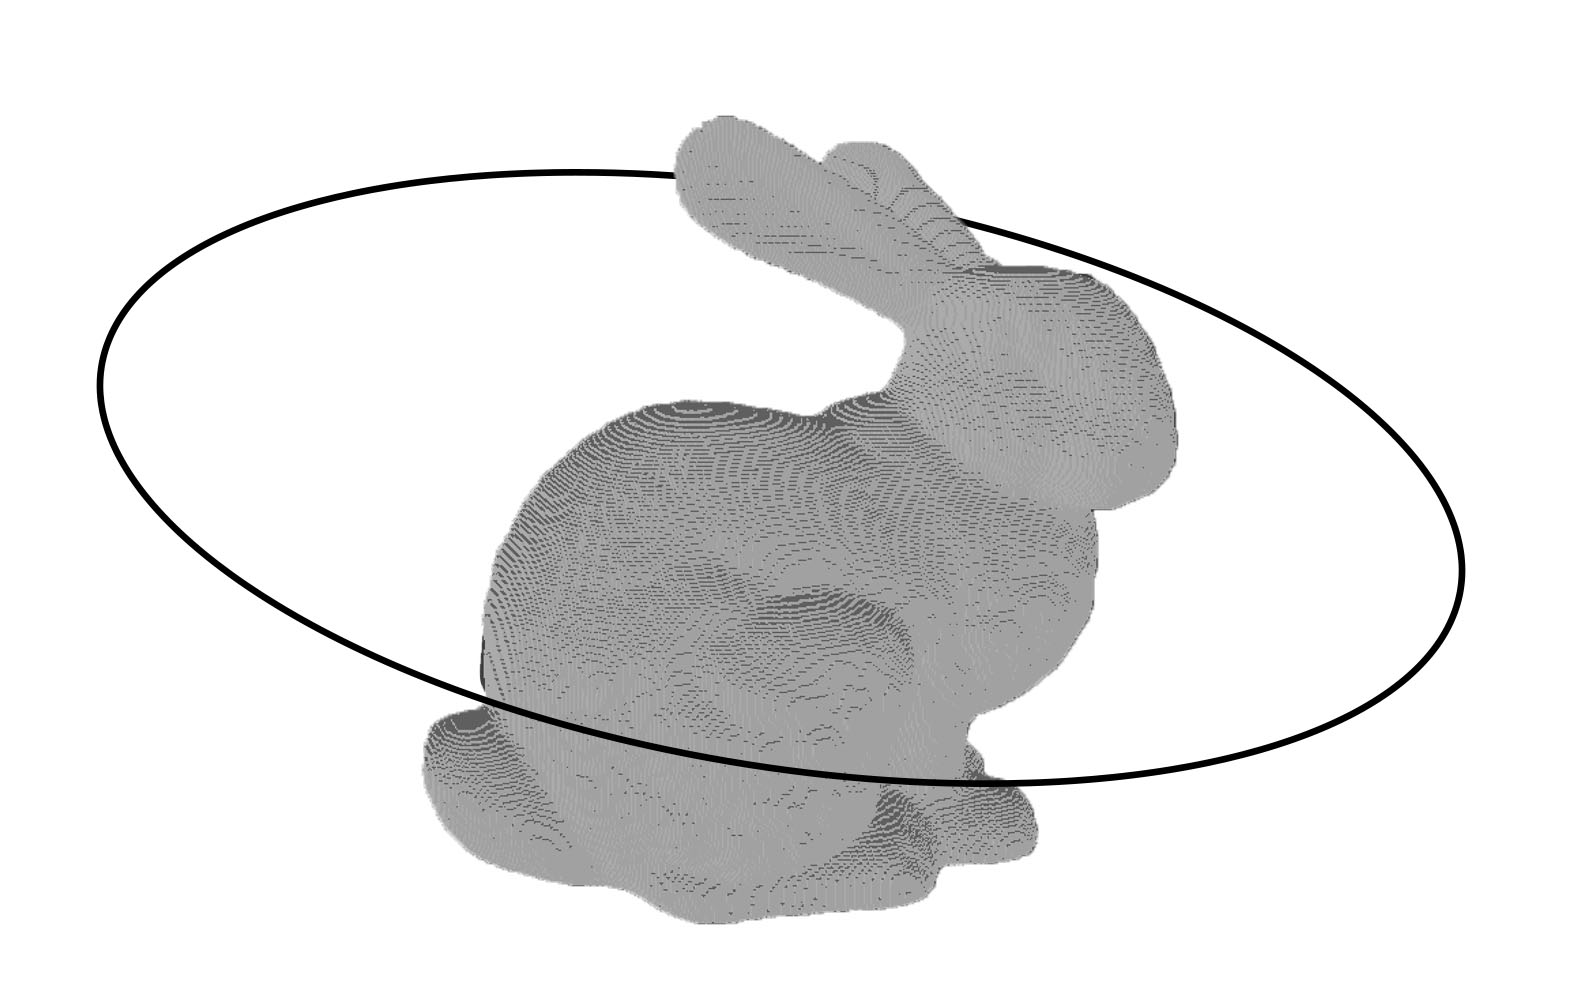
\includegraphics[width=200px]{images/graphics/test-anim-camera-path.jpg}
    \caption{During profiling, the camera is moved along an orbit around the voxel scene while being offset to compensate 
    for models, which behave differently when viewed from an angle. The visualization is not to scale, the models 
    were always completely visible and not culled by view frustum culling.}
    \label{fig:test-anim-camera-path}
\end{figure}

\noindent
Another aspect to consider is the model data structure. The voxel models are volumetric representations and thus 
not hollow. This leaves a large portion of the computation to be irrelevant and allows for the occlusion culling to 
optimize the data flow. Different types of models were used to challenge the culling algorithm in various ways. 
In concept, the culling should be optimal on large, dense models with even faces. Consequently, models with 
slopes and holes were tested to see how the best occluders can be computed for diverse geometry. Smaller models might 
also pose a challenge for the optimization, especially when the octree nodes cannot be filled completely. \\

\noindent
The resolution of the voxelization process played a central role in the experimentation process. For the experiment, 
the voxel scenes were constrained to be a power of two in length per axis, and a resolution of 
$\emph{256} \times \emph{256} \times \emph{256}$ was used for the performance profiling, resulting in a maximum of 
16,777,216 voxels. In practice, the maximum amount of voxels was limited by the data dispatch limitation mentioned in 
Chapter \ref{sec-implementation-limitations}.


\subsection*{Timings} \label{subsec-timings}

The time spent for various computations is relevant for the selection of the best algorithm. This is a central 
tool to see how the implementation performs overall in the context of the used framework. Consequently, the 
timings for all major pipeline steps were considered, as well as the overall time spent on \ac{CPU} and \ac{GPU} 
computations. \\

\noindent 
The overall framerate of the application was artificially clamped to 30, 60, or 120 \emph{Hz} by \emph{Diligent Engine}, 
depending on the connected monitor, which occasionally resulted in abrupt changes of frame times. This also means 
that the overall frame time was not reliably showing the \ac{CPU} workload. However, measuring only the internal render 
and update routines provided more reliable results. This is why the overall frame time isn't used for further analysis 
but is listed in Appendix \ref{cpt-appendix}.


\subsection*{Visibility and Culling} \label{subsec-visibility-and-culling}

In order to evaluate the general functionality and effectiveness of the pipeline, the voxel scene was analyzed 
with and without the occlusion culling applied. The amount of culled voxels was compared to the total amount of 
voxels, resulting in an overview of how much geometry could be culled for different scene setups. The same is 
valid for the amount of octree nodes. They could also be compared to the number of best occluders. The more best 
occluders present in a scene, the higher the probability to occlude other voxels or octree nodes. To evaluate 
the optimization during the depth prepass, the number of best occluders was compared to the number of voxels 
representing the geometry approximated by the best occluders, because it is favorable to have a small number of 
best occluders approximate a high number of voxels.\\


\subsection*{Measuring Tools} \label{subsec-measuring-tools}

To measure timings and data precisely, a few external tools were used. All tools are of industry standard 
and were therefore assumed to be mostly reliable. Still, measuring performance usually comes with a minimal 
overhead, which means that the results most likely vary in precision. Also, some of the tools provided 
various ways of sampling the data. Some data was measured while the profiled application was running, and 
other data was acquired by replaying the command list of the \ac{GPU}. Consequently, all measurements 
referring to one aspect of the application were compared against measurements using the same tool and 
configuration. \\

\noindent
For the collection of data output, \emph{RenderDoc} \cite{RenderDoc} was used. It is a free, MIT-licensed 
rendering debugger, widely used in the industry. For \emph{NVIDIA}-specific \ac{GPU} profiling, \emph{NVIDIA NSight} 
\cite{NSight} was used, which is another industry-standard profiling and debugging tool. It is only available for 
inspection of \emph{NVIDIA} graphics card computations but provided valuable insights into the rendering pipeline 
and hardware usage. The last tool used is \emph{Microsoft's PIX} \cite{PIX}, which is another performance debugging 
and profiling tool for \emph{Windows} platforms using \emph{Microsoft's DirectX} \ac{API}. \\

\noindent
The culling result measurements were directly sampled from the \emph{task shader} over the course of the testing 
animation, using \emph{RenderDoc} and \emph{PIX}. They were generally independent from the hardware and rather 
depended on the camera position and viewing angle as well as on model resolution. Also, the screen resolution 
affected the amount of mip maps generated for the \ac{HiZ} pyramid, so it was fixed to $1280 \times 900$ pixels. 
All of the aspects above were standardized for each model over all test runs.


\subsection*{Experimental Environment} \label{subsec-experimental-environment}

For the experiment, a modern hardware setup was used for performance profiling. All performance-related 
measurements were performed on Setup 1, outlined in Table \ref{tbl:hardware-setup}. Some measurements 
were performed on Setup 2, although none of those measurements were performance-related.

\begin{table}[h]          % System setup table
  \centering
    \begin{tabular}{|lll|}
        \hline
        \multicolumn{3}{|c|}{\textbf{Test setups}}                                                                              \\ \hline
        \multicolumn{1}{|l|}{}                     & \multicolumn{1}{l|}{\textbf{Setup 1}}          & \textbf{Setup 2}          \\ \hline
        \multicolumn{1}{|l|}{\textbf{System Type}} & \multicolumn{1}{l|}{Desktop}                   & Laptop                    \\
        \multicolumn{1}{|l|}{\textbf{CPU}}         & \multicolumn{1}{l|}{AMD Ryzen 9 9950X}         & Intel Ultra 7 155H        \\
        \multicolumn{1}{|l|}{\textbf{Cores}}       & \multicolumn{1}{l|}{16 (32)}                   & 16 (22)                   \\
        \multicolumn{1}{|l|}{\textbf{RAM}}         & \multicolumn{1}{l|}{96 GB}                     & 16 GB                     \\
        \multicolumn{1}{|l|}{\textbf{GPU}}         & \multicolumn{1}{l|}{NVIDIA GeForce RTX 4090}   & Intel Arc Graphics        \\
        \multicolumn{1}{|l|}{\textbf{VRAM}}        & \multicolumn{1}{l|}{24 GB}                     & 128 MB (+ 8972 MB shared) \\
        \multicolumn{1}{|l|}{\textbf{OS}}          & \multicolumn{1}{l|}{Windows 10}                & Windows 11                \\
        \multicolumn{1}{|l|}{\textbf{Model}}       & \multicolumn{1}{l|}{-}                         & ASUS Zenbook 14 (2024)    \\ \hline
    \end{tabular}
    \caption{The experimental setups used to profile the applications performance.}
    \label{tbl:hardware-setup}
\end{table}

\noindent
Note that the use of the mesh shading pipeline requires graphics cards that support the pipeline in the first place. 
For \emph{NVIDIA} \ac{GPU}s, this is the \emph{Turing} lineup (\emph{NVIDIA RTX 20 series}), and for \emph{AMD} cards, 
this would be the \emph{RDNA 2} lineup (\emph{AMD RX 6000 series}). \emph{Intel} \ac{GPU}s support the feature as 
well, starting from their first installment in the dedicated desktop \ac{GPU} series, \emph{Intel Arc}. \\


\section{Experimental Results}

In this section, the experimental results are presented and discussed for each model tested.
For each model, the culling results include data that isn't dependent on specific hardware. 
After that, the profiling measurements are discussed, which relate to the hardware setup 
presented in \ref{subsec-experimental-environment}. The data analysis is structured similarly 
for all models, comparing the \ac{PONOC} configuration to the \ac{PMOC} configuration. Finally, 
an overview is presented that summarizes all the relevant data in a compact visualization.


\subsection*{Best Occluder Selection}

To evaluate the best occluder selection, all models were tested in terms of the octree's query 
for the best occluders. This is an essential measure for evaluating the capability of the 
occlusion culling approach to work in dynamic scenes that change their voxel data in between 
frames. For the evaluation, a time budget of approximately 16.6 ms per frame is used as a 
reference budget, which is used to reach a framerate of 60 \emph{Hz} at runtime. The measured 
values for each tested scene are presented in Table \ref{tab:best-occluder-query}. 

\begin{table}[htbp]
  \begin{center}
    \begin{tabular}{|c|c|c|c|c|}
      \hline
      \textbf{}&\multicolumn{4}{|c|}{\textbf{Best Occluder Selection - $256^3$}} \\
      \cline{2-5} 
      \textbf{Scene} & \textbf{\textit{Voxel Count}}& \textbf{\textit{Best Occluder Count}}& \textbf{\textit{Hierarchy Width}}& \textbf{\textit{Time (ms)}} \\
      \hline
      Lucy        & 331,254   & 1600 & 2 / 8  & 0.317 \\
      Bunny       & 3,379,738 & 8256 & 8 / 8  & 3.752 \\
      Torus       & 2,311,006 & 7168 & 4 / 8  & 2.681 \\
      Terrain     & 953,362   & 6976 & 4 / 8  & 1.267 \\
      Hairball    & 1,652,435 & 5056 & 4 / 8  & 2.377 \\
      \hline
    \end{tabular}
    \caption{Measurements of best occluder query.}
  \label{tab:best-occluder-query}
  \end{center}
\end{table}

\noindent
The measurements show that each scene was processed in significantly less than 16.6 ms and the 
computation times scaled with the amount of voxels within the scene. The table additionally shows 
the octree hierarchy width. The hierarchy is limited in its depth by the maximum amount of voxels 
per octree node. However, its width is defined by the scene topology. The table shows how many of 
the first eight child nodes in the hierarchy are subdivided into more child nodes. While \emph{Lucy} 
only occupies two of the eight child nodes, the \emph{Bunny} model occupies all of the first eight 
child nodes.


\subsection*{Stanford Lucy}

The \emph{Lucy} model is tall and slim, which means that its volume is distributed more over one axis 
than over the other two axes. This is assumed to provide interesting insights into how such an object 
self-occludes the voxels when viewed from different perspectives. It also has a few narrow parts where 
no best occluders are expected.


\subsubsection*{Culling Results} \label{subsubsec-culling-results-lucy}

% --------------------------------------- LUCY 256 ---------------------------------------

\begin{figure}[!htb]              % Lucy 256 Culling Res
    \begin{center}
      \begin{tikzpicture}
        \begin{axis}[
            width=\linewidth, % Scale the plot to \linewidth
            height=100px,
            xlabel={Frames},
            ylabel={Computed Voxels},
            grid,
            xmin=0,
            xmax=2392,
            ymin=60000,
            ymax=160000,
            legend style={at={(0.5,1.7)}, anchor=north, legend columns=2},
          ]
          \addplot[blue, no marks, solid] table[col sep=comma, x=frame, y=visible_voxels]{./plotdata/lucy_256_voxels.csv};
          \addplot[red, no marks, solid] table[col sep=comma, x=frame, y=visible_voxels]{./plotdata/lucy_256_voxels_pmoc.csv};
          \addplot[blue, dotted, no marks, domain=0:2393, samples=50] {140842};
          \addplot[red, dotted, no marks, domain=0:2393, samples=50] {84082};
          \legend{Per-Octree Occlsion Culling, Per-Meshlet Occlusion Culling}
        \end{axis}
      \end{tikzpicture}
      \begin{tikzpicture}
        \begin{axis}[
            width=\linewidth, % Scale the plot to \linewidth
            height=100px,
            xlabel={Frames},
            ylabel={Computed Nodes},
            grid,
            xmin=0,
            xmax=2392,
            ymin=1800,
            ymax=4000,
            legend style={at={(0.5,1.7)}, anchor=north, legend columns=2},
          ]
          \addplot[blue, no marks, solid] table[col sep=comma, x=frame, x expr=\thisrow{frame} * 2392 / 2392, y=visible_nodes]{./plotdata/lucy_256_nodes.csv};
          \addplot[red, no marks, solid] table[col sep=comma, x=frame, x expr=\thisrow{frame} * 2392 / 2395, y=visible_nodes]{./plotdata/lucy_256_nodes_pmoc.csv};
          \addplot[blue, dotted, no marks, domain=0:2393, samples=50] {3460};
          \addplot[red, dotted, no marks, domain=0:2393, samples=50] {2483};
          \legend{Per-Octree Occlsion Culling, Per-Meshlet Occlusion Culling}
        \end{axis}
      \end{tikzpicture}
      \caption{\textbf{First:} The amount of visible voxels over the course of the test animation. \\
      \textbf{Second:} The amount of visible octree nodes over the course of the test animation.}
      \label{plt:lucy-256-culling-culling-results}
    \end{center}
  \end{figure}

% ----------------------------------------------------------------------------------------

\noindent
Figure \ref{plt:lucy-256-culling-culling-results} shows the amount of visible voxels and visible octree 
nodes for both occlusion culling configurations, as well as the average values represented by the dotted 
lines. \\

\noindent
The average amount of visible voxels was 140,842 for \ac{PONOC} and 84,082 for \ac{PMOC}, 
while the number of total voxels in the scene was 331,254. The average amount of visible 
octree nodes was 3,460 for \ac{PONOC} and 2,483 for \ac{PMOC}. The number of total octree 
nodes in the scene was 6,830. \\

\noindent
The measurements show that the \ac{PMOC} significantly reduced the amount of dispatched voxels and octree nodes. 
The amount of octree nodes decreased when using \ac{PMOC} because octree nodes could be culled, even when their 
corners were visible by the camera. Looking at the data over time, the amount of visible voxels and octree nodes
varies in a similar way. The curves are used to evaluate how well the scene fits the culling algorithm. This 
scene has a relatively even curve over time but of course, this is a dynamic measure and highly depends on the 
angle of the camera. Still, the compact, tall model seems to have provided a good amount of best occluders to 
occlude a relatively even number of voxels when viewed from the side. \\

\noindent
Considering the average amount of visible voxels for both culling configurations, \ac{PONOC} was able to cull 
$57.5\%$ of all voxels. On average, the \ac{PMOC} even managed to omit $74.6\%$ of all voxels. For \ac{PONOC},
the number of visible voxels diverged by a maximum of $17.83\%$ from the average value, and by $27.18\%$ for \ac{PMOC}. 
For the visible octree nodes, the variations were $14.80\%$ for \ac{PONOC} and $23.28\%$ for \ac{PMOC}.

\subsubsection*{CPU Performance Results} \label{subsubsec-cpu-performance-results-lucy}

\begin{figure}[!htb]              % Lucy renderTimes
  \begin{center}
    \begin{tikzpicture}
      \begin{axis}[
          width=\linewidth,
          height=100px,
          xlabel={Frames},
          ylabel={Update Time (s)},
          grid,
          xmin=0,
          xmax=2392,
          ymin=0,
          ymax=0.00005,
          legend style={at={(0.5,1.8)}, anchor=north, legend columns=2},
        ]
        \addplot[brown!60, no marks, solid] table[col sep=comma, x=frame, x expr=\thisrow{frame} * 2392 / 1648, y=time]{./plotdata/cpu/lucy_256_updateTime_nocull.csv};
        \addplot[blue, no marks, solid] table[col sep=comma, x=frame, x expr=\thisrow{frame} * 2392 / 1863, y=time]{./plotdata/cpu/lucy_256_updateTime_pooc.csv};
        \addplot[red, no marks, solid] table[col sep=comma, x=frame, x expr=\thisrow{frame} * 2392 / 1867, y=time]{./plotdata/cpu/lucy_256_updateTime.csv};
        \legend{No Occlusion Culling, Per-Octree Occlsion Culling, Per-Meshlet Occlusion Culling}
      \end{axis}
    \end{tikzpicture}
    \begin{tikzpicture}
      \begin{axis}[
          width=\linewidth,
          height=100px,
          xlabel={Frames},
          ylabel={Render Time (s)},
          grid,
          xmin=0,
          xmax=2392,
          ymin=0,
          ymax=0.00025,
          legend style={at={(0.5,1.8)}, anchor=north, legend columns=2},
        ]
        \addplot[brown!60, no marks, solid] table[col sep=comma, x=frame, x expr=\thisrow{frame} * 2392 / 1648, y=time]{./plotdata/cpu/lucy_256_renderTime_nocull.csv};
        \addplot[blue, no marks, solid] table[col sep=comma, x=frame, x expr=\thisrow{frame} * 2392 / 1863, y=time]{./plotdata/cpu/lucy_256_renderTime_pooc.csv};
        \addplot[red, no marks, solid] table[col sep=comma, x=frame, x expr=\thisrow{frame} * 2392 / 1867, y=time]{./plotdata/cpu/lucy_256_renderTime.csv};
        \legend{No Occlusion Culling, Per-Octree Occlsion Culling, Per-Meshlet Occlusion Culling}
      \end{axis}
    \end{tikzpicture}
    \caption{Overview of the render times over the course of the test animation. The first graph shows the time 
    each frame took to execute the \emph{Update()} function on the \ac{CPU}. The second graph shows the time each 
    frame took to execute the \emph{Render()} function on the \ac{CPU}. This includes the completion of the 
    \ac{GPU} computations.}
    \label{plt:lucy-256-culling-cpu-time}
  \end{center}
\end{figure}

\noindent
Figure \ref{plt:lucy-256-culling-cpu-time} shows the \ac{CPU} times spent on the \emph{Update()} and \emph{Render()}
routines. The \emph{Update()} function includes updating the camera's view and projection matrices. This function was 
expected to be static in runtime, regardless of the culling configuration. The graph shows that this is generally 
correct, as both are not significantly diverging. Nevertheless, there are small differences in the frame times, 
especially when comparing both culling configurations to the base pipeline without culling enabled. Within the last 
800 frames, the base pipeline seems to have had longer update times. The differences cannot be clearly attributed to 
any difference in the pipelines since the code was identical for all measured configurations. \\

\noindent
The \emph{Render()} function includes the rendering process, the dispatch of the depth prepass, and the drawing of the 
debugging \ac{UI}. Similar to the \emph{Update()} routine, the \emph{Render()} function doesn't change significantly 
between the configurations. Small differences are visible when comparing both culling configurations to the base 
pipeline without culling. There were small frame time spikes between frames 700 and 900. However, it is not obvious 
why these differences occurred. Minor differences might be attributed to the varying \ac{GPU} times presented below, 
but since \ac{GPU} work is usually running asynchronously, it is hard to point to a particular reason in this case. \\

\noindent
In general, the time spent on the most significant \ac{CPU} computations was pretty much static for this specific 
model. This result is as expected, since most of the work was executed on the \ac{GPU} anyway, including the creation 
of the voxel meshes. After all, this approach is \ac{GPU}-driven at its core, so the bandwidth is small, and the culling 
completely happens on the \ac{GPU} end of the pipeline.

\subsubsection*{GPU Performance Results} \label{subsubsec-gpu-performance-results-lucy}

\begin{figure}[!htbp]      % Lucy GPU Results
  \centering
  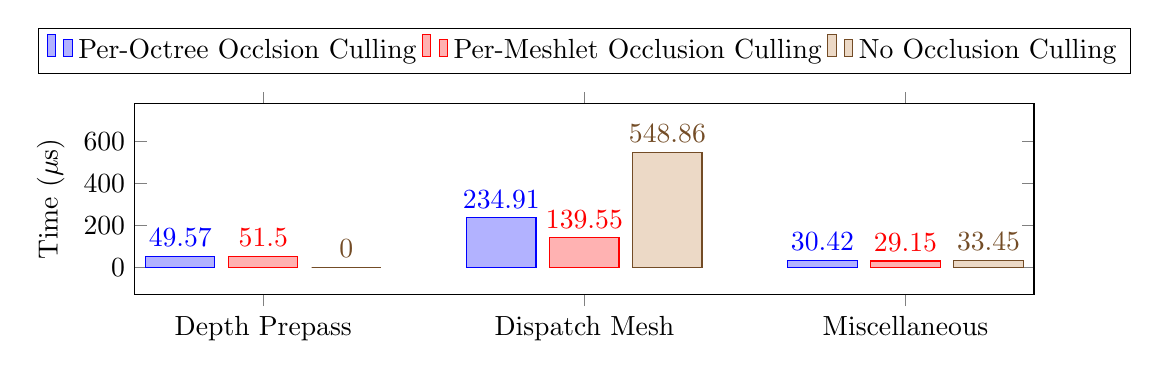
\begin{tikzpicture}
    \begin{axis}[
        height=4cm,
        width=13cm,
        x tick label style={/pgf/number format/1000 sep=},
        ylabel={Time ($\mu$s)},
        legend style={at={(0.5,1.4)}, anchor=north, legend columns=-1},
        symbolic x coords={DepthPrepass, DispatchMesh, Misc},
        xticklabels={Depth Prepass, Dispatch Mesh, Miscellaneous},
        xtick=data,
        ybar=0.4,
        bar width=25pt,
        ymin=0,
        ymax=650,
        nodes near coords,
        enlargelimits=0.2,
    ]
    \addplot+[bar shift=-30pt] coordinates {(DepthPrepass,49.57) (DispatchMesh,234.91) (Misc,30.42)};
    \addplot+[bar shift=0pt] coordinates {(DepthPrepass,51.50) (DispatchMesh,139.55) (Misc,29.1476)};
    \addplot+[bar shift=30pt] coordinates {(DepthPrepass,0) (DispatchMesh,548.86) (Misc,33.45)};
    \legend{Per-Octree Occlsion Culling, Per-Meshlet Occlusion Culling, No Occlusion Culling}
    \end{axis}
  \end{tikzpicture}

  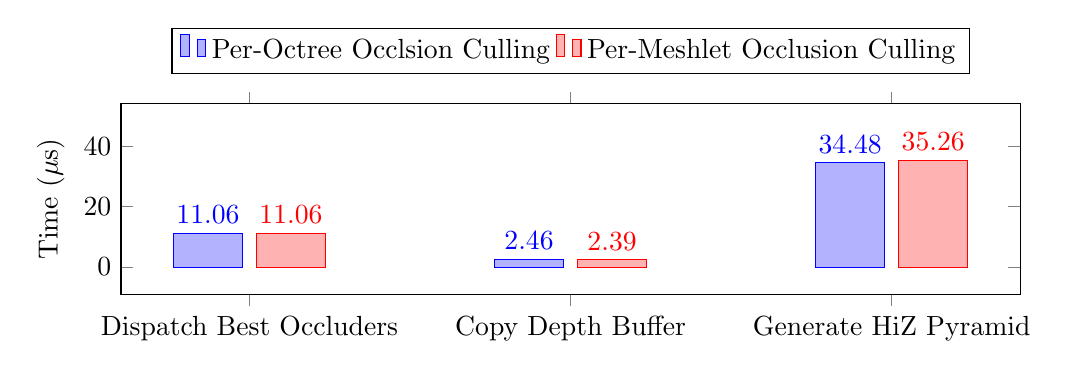
\begin{tikzpicture}
    \begin{axis}[
        height=4cm,
        width=13cm,
        x tick label style={/pgf/number format/1000 sep=},
        ylabel={Time ($\mu$s)},
        legend style={at={(0.5,1.4)}, anchor=north, legend columns=-1},
        symbolic x coords={DispatchBestOccluders, CopyTex, GenMipChain},
        xticklabels={Dispatch Best Occluders, Copy Depth Buffer, Generate \ac{HiZ} Pyramid},
        xtick=data,
        ybar=0.4,
        bar width=25pt,
        ymin=0,
        ymax=45,
        nodes near coords,
        enlargelimits=0.2,
    ]
    \addplot+[bar shift=-15pt] coordinates {(DispatchBestOccluders,11.06) (CopyTex,2.46) (GenMipChain,34.48)};
    \addplot+[bar shift=15pt] coordinates {(DispatchBestOccluders,11.06) (CopyTex,2.39) (GenMipChain,35.26)};
    \legend{Per-Octree Occlsion Culling, Per-Meshlet Occlusion Culling}
    \end{axis}
  \end{tikzpicture}

  \caption{\textbf{First:} The complete time measured on the \ac{GPU}. The \emph{Depth Prepass} is the extra overhead 
  introduced by the \ac{HZB}. The \emph{Dispatch Mesh} is the drawing of the meshes, including the occlusion 
  culling. \emph{Miscellaneous} includes a small amount of \emph{Barriers} used for synchronization and the 
  rendering of some debug \ac{UI}. It is considered to be more or less static in computation time and is not 
  part of the actual algorithm measured in this experiment. \textbf{Second:} The time measured in the \emph{Depth Prepass}. 
  The \emph{Dispatch Best Occluders} is the drawing to the depth buffer. The \emph{Copy Depth Buffer} computation 
  copies the depth buffers content into the final \ac{HiZ} resource. Finally, \emph{Generate HiZ Pyramid} shows 
  the \ac{HiZ} creation, which is done sequentially.}
\end{figure}

\noindent
On the \ac{GPU}, the \ac{PMOC} turned out to be faster in computation. As the occlusion culling algorithm 
intended, the time spent drawing the meshes could be reduced by $30\%$ on average for this particular model. 
Compared to the base pipeline featuring no culling, the performance on the \ac{GPU} side was increased by 
$58.2 \%$ using \ac{PONOC} and $74.6\%$ using \ac{PMOC}. \\

\noindent
The comparison of the depth prepass shows a small difference in computation time. The per-octree node configuration 
terminated faster by $1.93$ microseconds on average. In this case, the difference was created by small deviations in 
copying the depth buffer and computing the mip maps. All prepass steps were identical between both culling 
configurations.

\subsubsection*{Overdraw}

\begin{figure}[!htbp]
  \centering
  
\includegraphics[height=100px]{images/graphics/overdraw-lucy1-nocull.png}
  
\includegraphics[height=100px]{images/graphics/overdraw-lucy1-pooc.png}
  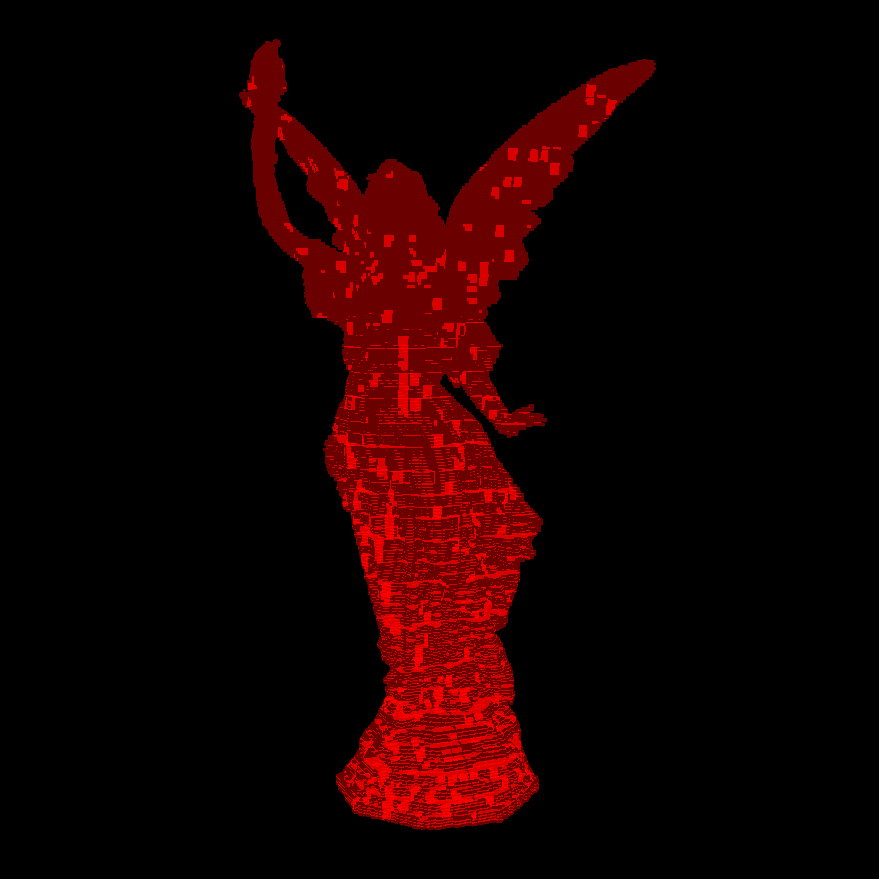
\includegraphics[height=100px]{images/graphics/overdraw-lucy1-pmoc.png}
  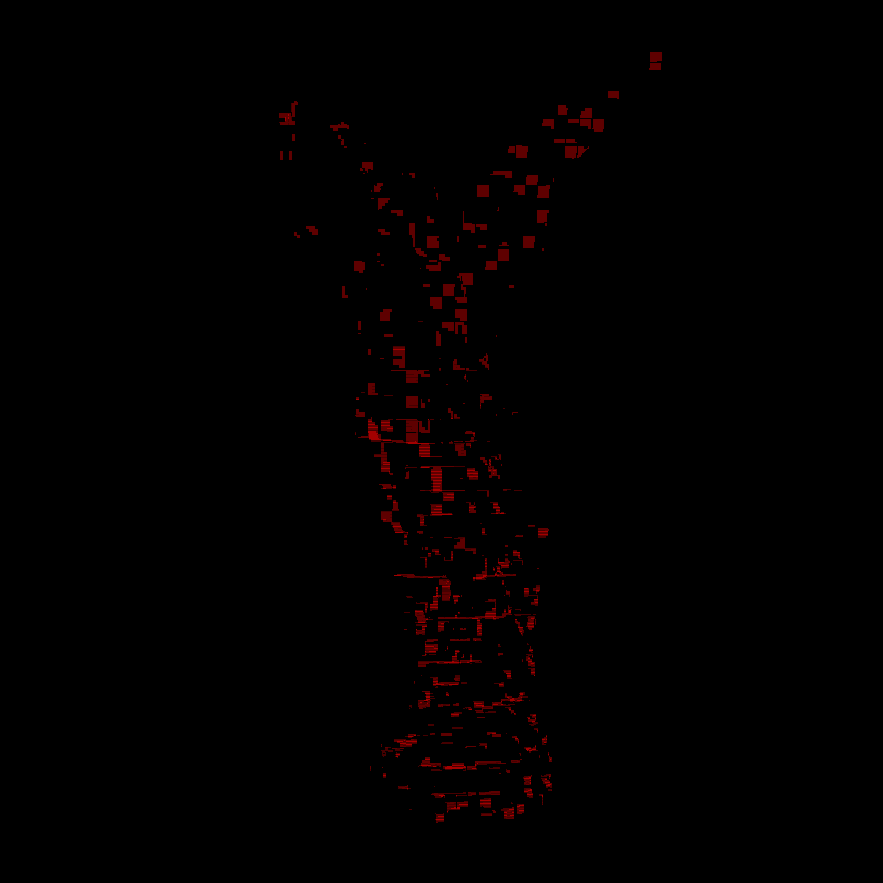
\includegraphics[height=100px]{images/graphics/overdraw-lucy1-diff.png}

  \begin{subfigure}{100px}
    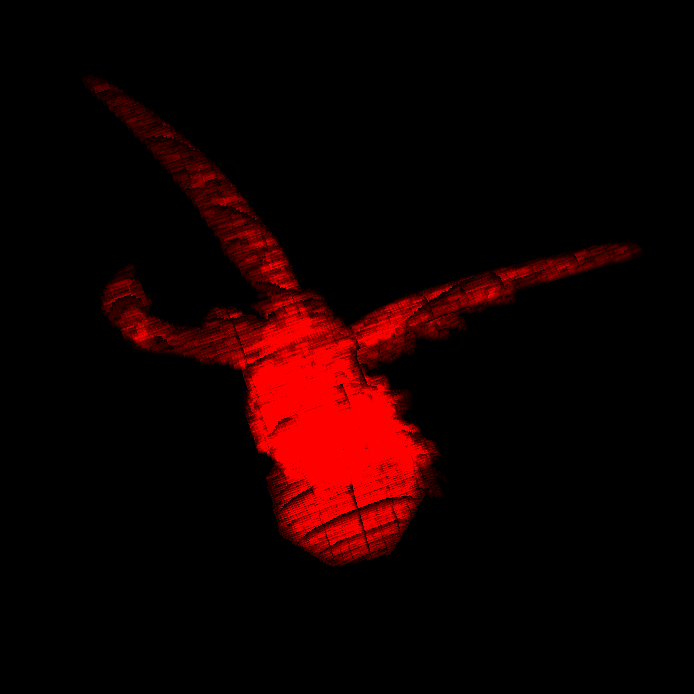
\includegraphics[height=100px]{images/graphics/overdraw-lucy2-nocull.png}
    \caption{}
    \parbox{\linewidth}{\centering\footnotesize No Occlusion\\Culling}
  \end{subfigure}
  \begin{subfigure}{100px}
    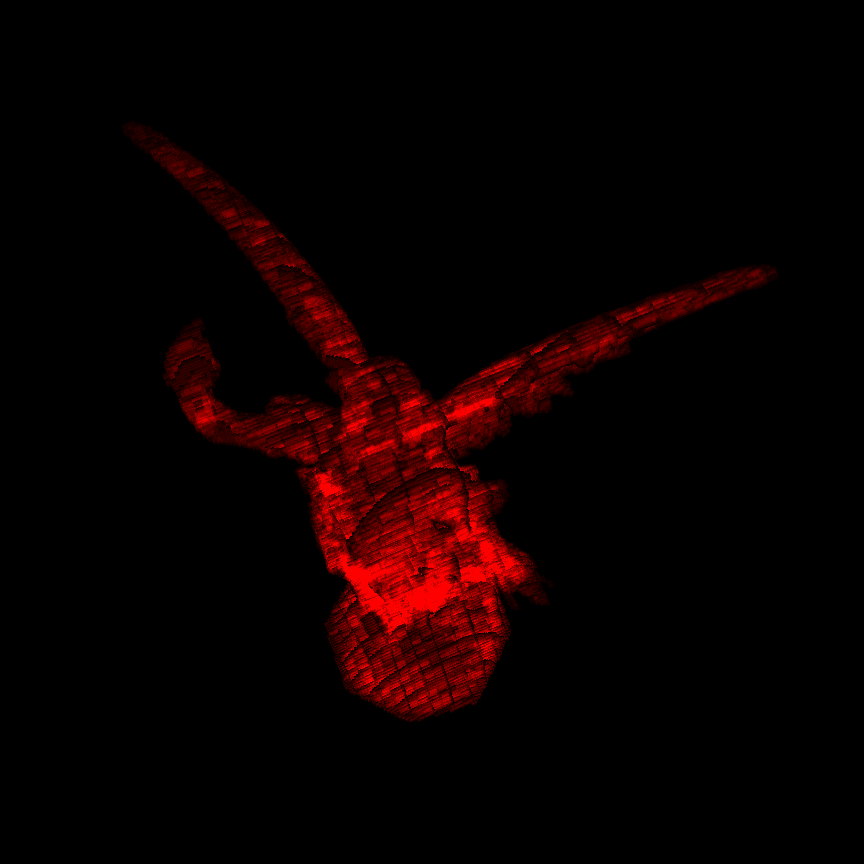
\includegraphics[height=100px]{images/graphics/overdraw-lucy2-pooc.png}
    \caption{}
    \parbox{\linewidth}{\centering\footnotesize Per-Octree Node\\Occlusion Culling}
  \end{subfigure}
  \begin{subfigure}{100px}
    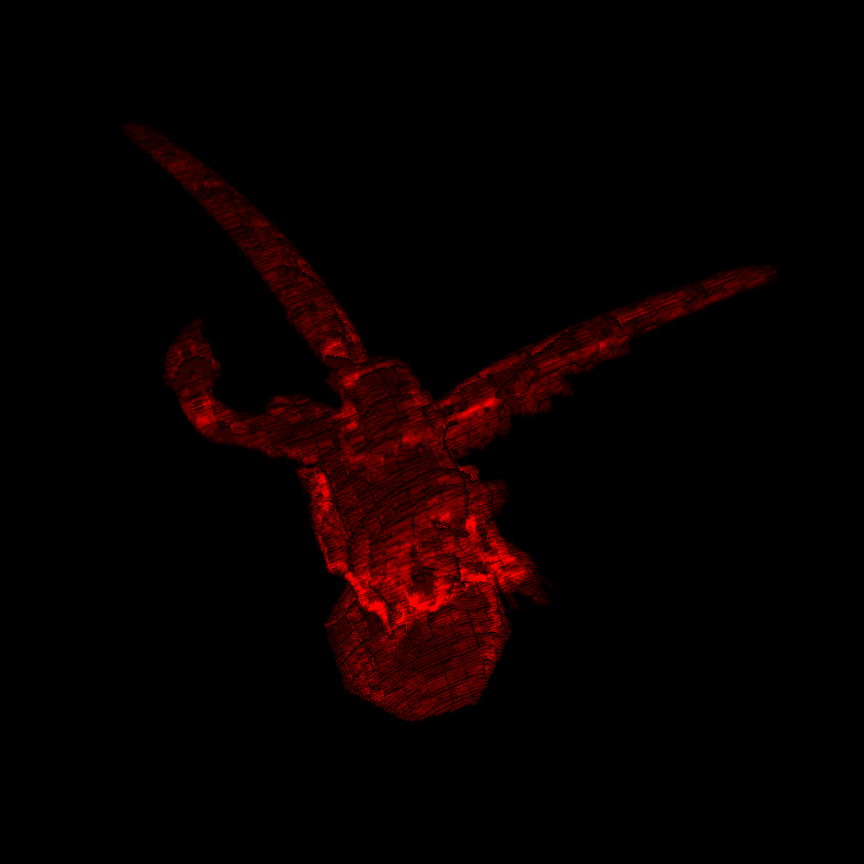
\includegraphics[height=100px]{images/graphics/overdraw-lucy2-pmoc.png}
    \caption{}
    \parbox{\linewidth}{\centering\footnotesize Per-Meshlet\\Occlusion Culling}
  \end{subfigure}
  \begin{subfigure}{100px}
    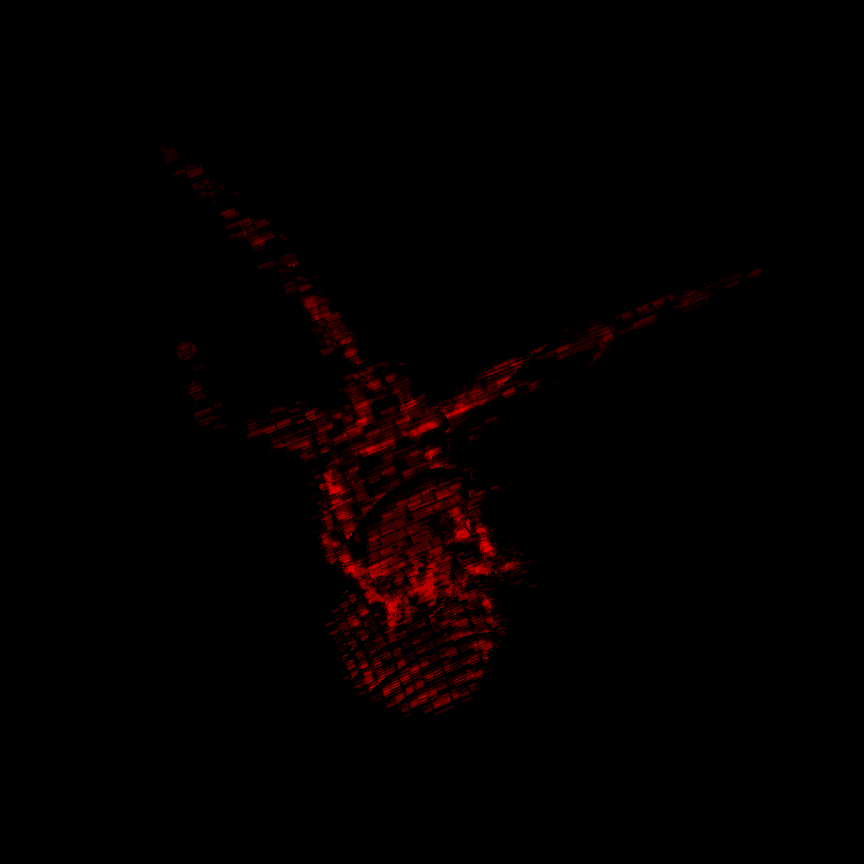
\includegraphics[height=100px]{images/graphics/overdraw-lucy2-diff.png}
    \caption{}
    \parbox{\linewidth}{\centering\footnotesize Difference\\(b) vs. (c)}
  \end{subfigure}

  \caption{Overdraw of the pixels from two different camera angles. 
  The image values are enhanced for better visualization.}
  \label{fig:lucy-overdraw}
\end{figure}

\noindent
Figure \ref{fig:lucy-overdraw} shows that the \ac{PONOC} had more overdrawn pixels than the \ac{PMOC} configuration. 
While the \ac{PONOC} resulted in a maximum overdraw of 38 draws per pixel, the \ac{PMOC} was able to reduce this to 
a maximum of 27 draws. The comparison measurement without occlusion culling resulted in a maximum of 78 draws. The 
side view featured only a maximum of 7 draws per pixel in both configurations and was in general less prone to overdraw.
For both camera angles, the difference visualization shows that the \ac{PMOC} configuration was able to decrease overdraw. 

\clearpage



\subsection*{Stanford Bunny}

The \emph{Stanford Bunny} is a large and dense model with a lot of voxels in any possible resolution.
It also has different features to it, one of them being the curved surface, resulting in a lot of octree 
nodes not being filled completely. On the other hand, because of its large volume, the model is assumed 
to be efficient when rendering the best occluders, aggregating a lot of smaller octree nodes to larger 
approximations.

\subsubsection*{Culling Results} \label{subsubsec-culling-results-bunny}

% --------------------------------------- BUNNY 256 --------------------------------------

\begin{figure}[!htb]              % Bunny 256 Voxels Test Anim
    \begin{center}
      \begin{tikzpicture}
        \begin{axis}[
            width=\linewidth, % Scale the plot to \linewidth
            height=100px,
            xlabel={Frames},
            ylabel={Computed Voxels},
            grid,
            xmin=0,
            xmax=1186,
            ymin=100000,
            ymax=500000,
            legend style={at={(0.5,1.7)}, anchor=north, legend columns=2},
          ]
          \addplot[blue, no marks, solid] table[col sep=comma, x=frame, x expr=\thisrow{frame} * 1186 / 1186, y=visible_voxels]{plotdata/bunny_256_voxels.csv};
          \addplot[red, no marks, solid] table[col sep=comma, x=frame, x expr=\thisrow{frame} * 1186 / 1490, y=visible_voxels]{plotdata/bunny_256_voxels_pmoc.csv};
          \addplot[blue, dotted, no marks, domain=0:1186, samples=50] {385210};
          \addplot[red, dotted, no marks, domain=0:1186, samples=50] {180266};
          \legend{Per-Octree Occlsion Culling, Per-Meshlet Occlusion Culling}
        \end{axis}
      \end{tikzpicture}

      \begin{tikzpicture}
        \begin{axis}[
            width=\linewidth, % Scale the plot to \linewidth
            height=100px,
            xlabel={Frames},
            ylabel={Computed Nodes},
            grid,
            xmin=0,
            xmax=1186,
            ymin=3000,
            ymax=10000,
            legend style={at={(0.5,1.7)}, anchor=north, legend columns=2},
          ]
          \addplot[blue, no marks, solid] table[col sep=comma, x=frame, x expr=\thisrow{frame} * 1186 / 1186, y=visible_nodes]{./plotdata/bunny_256_nodes.csv};
          \addplot[red, no marks, solid] table[col sep=comma, x=frame, x expr=\thisrow{frame} * 1186 / 1490, y=visible_nodes]{./plotdata/bunny_256_nodes_pmoc.csv};
          \addplot[blue, dotted, no marks, domain=0:1186, samples=50] {8519};
          \addplot[red, dotted, no marks, domain=0:1186, samples=50] {5415};
          \legend{Per-Octree Occlsion Culling, Per-Meshlet Occlusion Culling}
        \end{axis}
      \end{tikzpicture}
    \end{center}

      \caption{\textbf{First:} The amount of visible voxels over the course of the test animation. \\
      \textbf{Second:} The amount of visible octree nodes over the course of the test animation.}
      \label{plt:bunny-256-culling-res-voxels}
  \end{figure}
% ----------------------------------------------------------------------------------------

\noindent
Figure \ref{plt:bunny-256-culling-res-voxels} shows the amount of visible voxels and visible 
octree nodes for both occlusion culling configurations, as well as the average values represented 
by the dotted lines. \\

\noindent
The average amount of visible voxels was 385,210 for \ac{PONOC} and 180,266 for \ac{PMOC},
while the number of total voxels in the scene was 3,379,738. The average amount of visible 
octree nodes was 8,519 for \ac{PONOC} and 5,415 for \ac{PMOC}. The number of total octree 
nodes in the scene was 57,481. \\

\noindent
The measurements show that the \emph{Stanford Bunny} considerably benefitted from both occlusion 
culling configurations, and the most significant reduction of visible voxels resulted from the use 
of \ac{PMOC}. The average culling ratio was $88.6\%$ for the \ac{PONOC} and $94.6\%$ for the 
\ac{PMOC}. For \ac{PONOC}, the number of visible voxels diverged by a maximum of $30.88\%$ from 
the average value, and by $23.01\%$ for \ac{PMOC}. For the visible octree nodes, the variations were 
$24.61\%$ for \ac{PONOC} and $39.78\%$ for \ac{PMOC}.

\subsubsection*{CPU Performance Results} \label{subsubsec-cpu-performance-results-bunny}

\begin{figure}[!htb]              % Bunny cpu
  \begin{center}
    \begin{tikzpicture}
      \begin{axis}[
          width=\linewidth,
          height=100px,
          xlabel={Frames},
          ylabel={Update Time (s)},
          grid,
          xmin=0,
          xmax=1186,
          ymin=0,
          ymax=0.00005,
          legend style={at={(0.5,1.8)}, anchor=north, legend columns=2},
        ]
        \addplot[brown!60, no marks, solid] table[col sep=comma, x=frame, x expr=\thisrow{frame} * 1186 / 1236, y=time]{./plotdata/cpu/bunny_256_updateTime_nocull.csv};
        \addplot[blue, no marks, solid]  table[col sep=comma, x=frame, x expr=\thisrow{frame} * 1186 / 1574, y=time]{./plotdata/cpu/bunny_256_updateTime_pooc.csv};
        \addplot[red, no marks, solid] table[col sep=comma, x=frame, x expr=\thisrow{frame} * 1186 / 1700, y=time]{./plotdata/cpu/bunny_256_updateTime.csv};
        \legend{No Occlusion Culling, Per-Octree Occlsion Culling, Per-Meshlet Occlusion Culling}
      \end{axis}
    \end{tikzpicture}
    \begin{tikzpicture}
      \begin{axis}[
          width=\linewidth,
          height=100px,
          xlabel={Frames},
          ylabel={Render Time (s)},
          grid,
          xmin=0,
          xmax=1186,
          ymin=0,
          ymax=0.00025,
          legend style={at={(0.5,1.8)}, anchor=north, legend columns=2},
        ]
        \addplot[brown!60, no marks, solid] table[col sep=comma, x=frame, x expr=\thisrow{frame} * 1186 / 1236, y=time]{./plotdata/cpu/bunny_256_renderTime_nocull.csv};
        \addplot[blue, no marks, solid] table[col sep=comma, x=frame, x expr=\thisrow{frame} * 1186 / 1574, y=time]{./plotdata/cpu/bunny_256_renderTime_pooc.csv};
        \addplot[red, no marks, solid] table[col sep=comma, x=frame, x expr=\thisrow{frame} * 1186 / 1700, y=time]{./plotdata/cpu/bunny_256_renderTime.csv};
        \legend{No Occlusion Culling, Per-Octree Occlsion Culling, Per-Meshlet Occlusion Culling}
      \end{axis}
    \end{tikzpicture}
  \end{center}
    \caption{Overview of the render times over the course of the test animation. The first graph shows the time 
    each frame took to execute the \emph{Update()} function on the \ac{CPU}. The second graph shows the time each 
    frame took to execute the function \emph{Render()} on the \ac{CPU}. This includes the completion of the 
    \ac{GPU} computations.}
    \label{plt:bunny-256-culling-cpu-time}
\end{figure}


\noindent
Figure \ref{plt:bunny-256-culling-cpu-time} shows that there are no significant differences in render and update times.
There were occasional spikes in different frames, but mostly both configurations showed similar execution times. A 
difference between the culling configurations is visible between frames 280 and 380 in the \emph{Render()} routine. 
Here, the \ac{PMOC} was able to achieve lower render times on the \ac{CPU} compared to the \ac{PONOC} configuration. 
Another difference is visible between the base pipeline and both occlusion culling pipelines. For the first quarter 
of the test animation, the occlusion culling pipelines performed better than the base pipeline during the \emph{Render()} 
function. The differences might be caused by shorter \ac{GPU} times, but no final evaluation can be made in this case. 
Ultimately, the \ac{CPU} times do not show clear differences that can be attributed to any particular difference in 
the pipeline.

\subsubsection*{GPU Performance Results} \label{subsubsec-gpu-performance-results-bunny}

\begin{figure}[!htb]
  \centering
  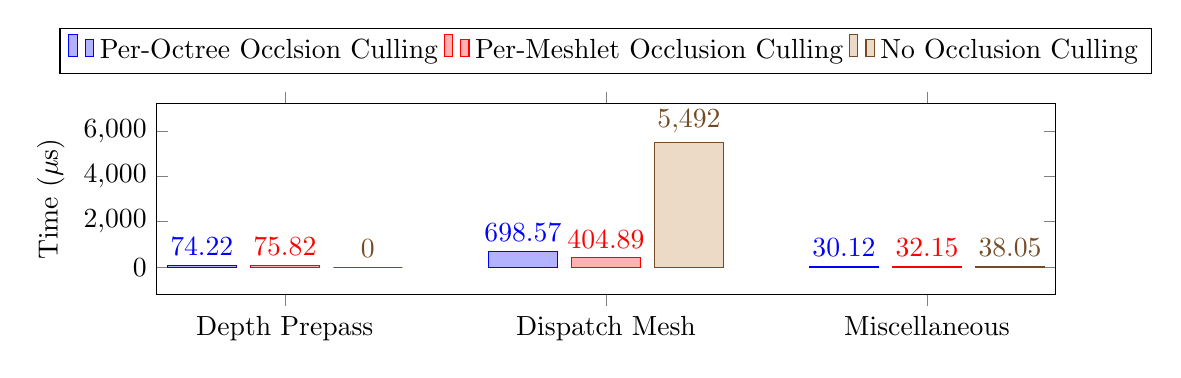
\begin{tikzpicture}
    \begin{axis}[
        height=4cm,
        width=13cm,
        x tick label style={/pgf/number format/1000 sep=},
        ylabel={Time ($\mu$s)},
        legend style={at={(0.5,1.4)}, anchor=north, legend columns=-1},
        symbolic x coords={DepthPrepass, DispatchMesh, Misc},
        xticklabels={Depth Prepass, Dispatch Mesh, Miscellaneous},
        xtick=data,
        ybar=0.4,
        bar width=25pt,
        ymin=0,
        ymax=6000,
        nodes near coords,
        enlargelimits=0.2,
    ]
    \addplot+[bar shift=-30pt] coordinates {(DepthPrepass,74.22) (DispatchMesh,698.57) (Misc,30.12)};
    \addplot+[bar shift=0pt] coordinates {(DepthPrepass,75.82) (DispatchMesh,404.89) (Misc,32.1526)};
    \addplot+[bar shift=30pt] coordinates {(DepthPrepass,0) (DispatchMesh,5492.00) (Misc,38.0522)};
    \legend{Per-Octree Occlsion Culling, Per-Meshlet Occlusion Culling, No Occlusion Culling}
    \end{axis}
  \end{tikzpicture}

  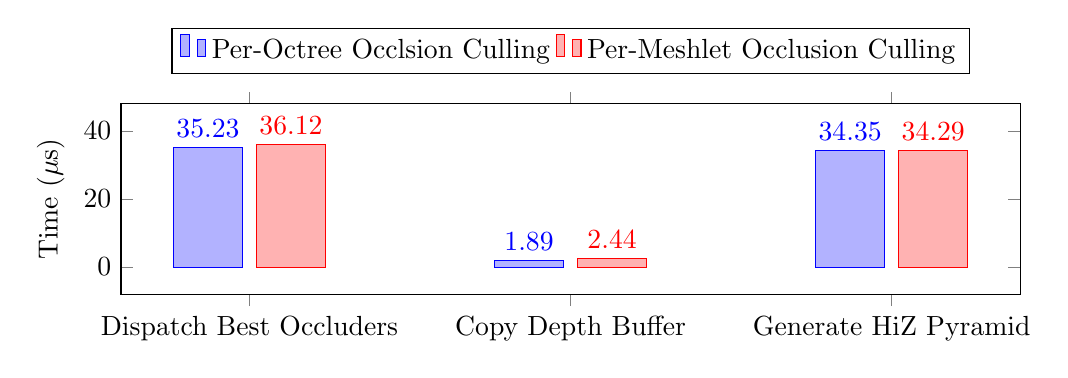
\begin{tikzpicture}
    \begin{axis}[
        height=4cm,
        width=13cm,
        x tick label style={/pgf/number format/1000 sep=},
        ylabel={Time ($\mu$s)},
        legend style={at={(0.5,1.4)}, anchor=north, legend columns=-1},
        symbolic x coords={DispatchBestOccluders, CopyTex, GenMipChain},
        xticklabels={Dispatch Best Occluders, Copy Depth Buffer, Generate \ac{HiZ} Pyramid},
        xtick=data,
        ybar=0.4,
        bar width=25pt,
        ymin=0,
        ymax=40,
        nodes near coords,
        enlargelimits=0.2,
    ]
    \addplot+[bar shift=-15pt] coordinates {(DispatchBestOccluders,35.23) (CopyTex,1.89) (GenMipChain,34.35)};
    \addplot+[bar shift=15pt] coordinates {(DispatchBestOccluders,36.12) (CopyTex,2.44) (GenMipChain,34.29)};
    \legend{Per-Octree Occlsion Culling, Per-Meshlet Occlusion Culling}
    \end{axis}
  \end{tikzpicture}

  \caption{\textbf{First:} The complete time measured on the \ac{GPU}. The \emph{Depth Prepass} is the extra 
  overhead introduced by the \ac{HZB}. The \emph{Dispatch Mesh} is the drawing of the meshes, including the 
  occlusion culling. \emph{Miscellaneous} includes a small amount of \emph{Barriers} used for synchronization 
  and the rendering of some debug \ac{UI}. It is considered to be more or less static in computation time and 
  is not part of the actual algorithm measured in this experiment. \textbf{Second:} The time measured in the 
  \emph{Depth Prepass}. The \emph{Dispatch Best Occluders} is the drawing to the depth buffer. The 
  \emph{Copy Depth Buffer} computation copies the depth buffers content into the final \ac{HiZ} resource. 
  Finally, \emph{Generate HiZ Pyramid} shows the \ac{HiZ} creation, which is done sequentially.}
\end{figure}

\noindent
The \ac{GPU} performance shows a significant difference when comparing both configurations. The \ac{PMOC} 
was able to decrease the time spent on \emph{DispatchMesh} by $36.1\%$ on average as compared to the 
\ac{PONOC}. On closer inspection, the depth prepass showed a minor difference in runtime. The difference 
is 1.6 microseconds, mostly due to differences in \ac{HiZ} dispatch and depth buffer copy. \\

\noindent
Both culling configurations decreased the time spent on the \ac{GPU} compared to the base pipeline by 
$85.5\%$ and $90.7\%$, respectively.

\subsubsection*{Overdraw} \label{subsubsec-overdraw-bunny}

\begin{figure}[!htb]
  \centering
  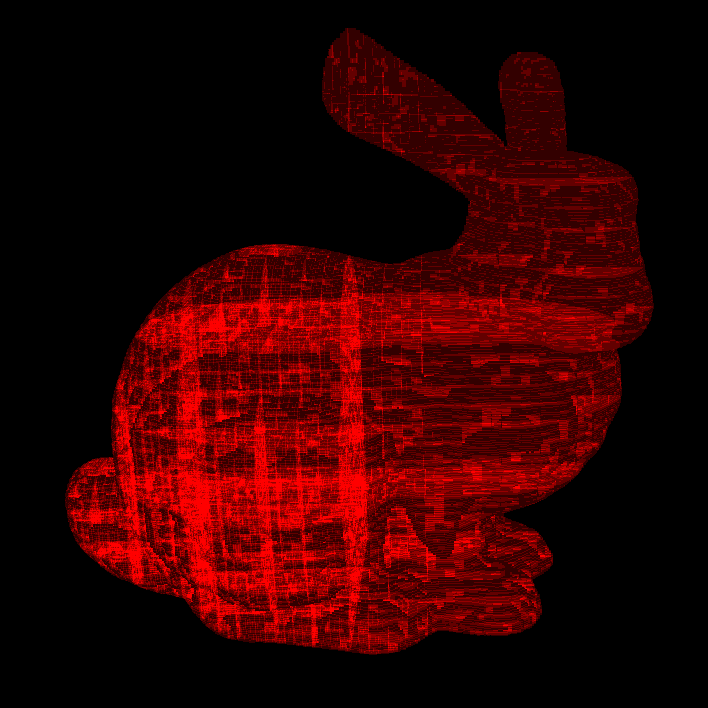
\includegraphics[width=100px]{images/graphics/overdraw-bunny1-nocull.png}
  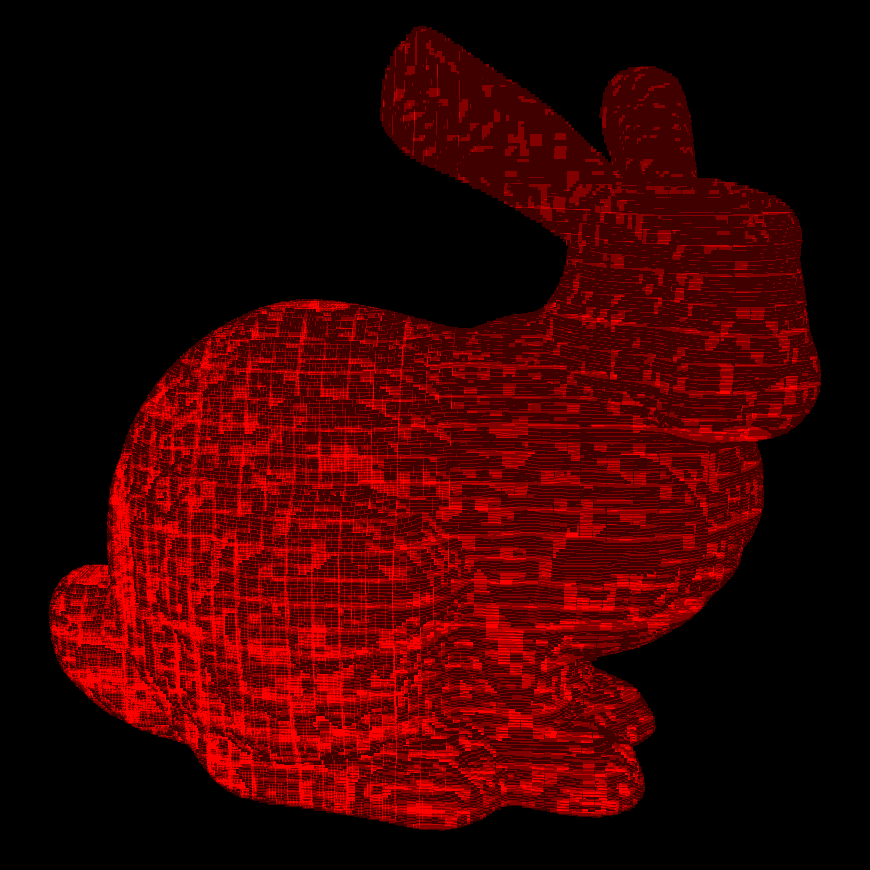
\includegraphics[width=100px]{images/graphics/overdraw-bunny1-pooc.png}
  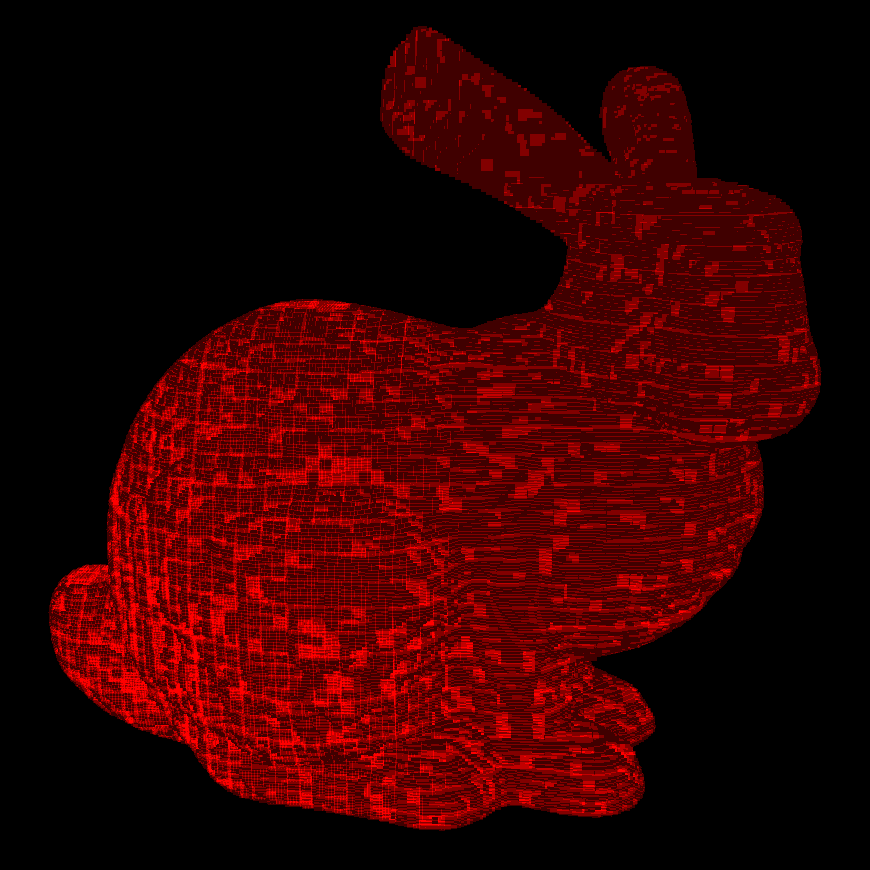
\includegraphics[width=100px]{images/graphics/overdraw-bunny1-pmoc.png}
  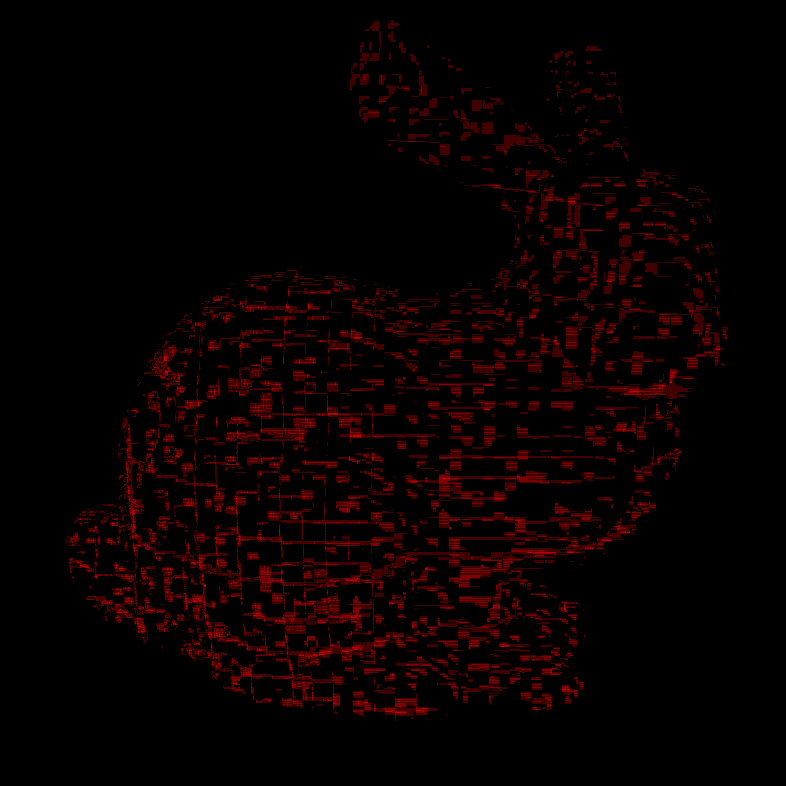
\includegraphics[width=100px]{images/graphics/overdraw-bunny1-diff.png}

  \begin{subfigure}{100px}
    
\includegraphics[width=100px]{images/graphics/overdraw-bunny2-nocull.png}
    \caption{}
    \parbox{\linewidth}{\centering\footnotesize No Occlusion\\Culling}
  \end{subfigure}
  \begin{subfigure}{100px}
    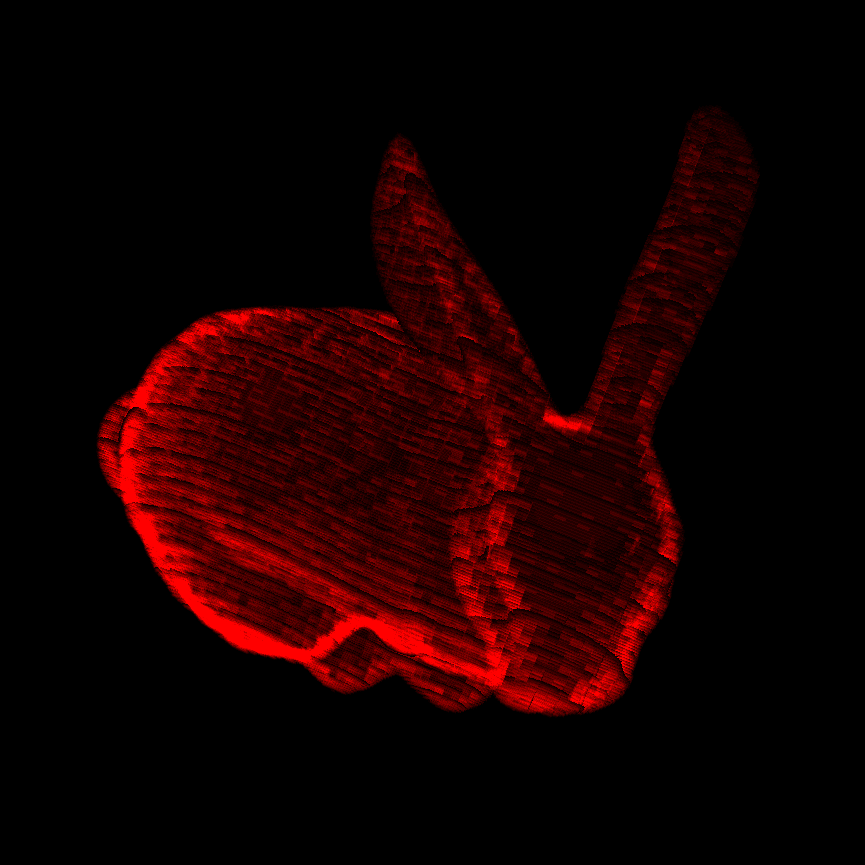
\includegraphics[width=100px]{images/graphics/overdraw-bunny2-pooc.png}
    \caption{}
    \parbox{\linewidth}{\centering\footnotesize Per-Octree Node\\Occlusion Culling}
  \end{subfigure}
  \begin{subfigure}{100px}
    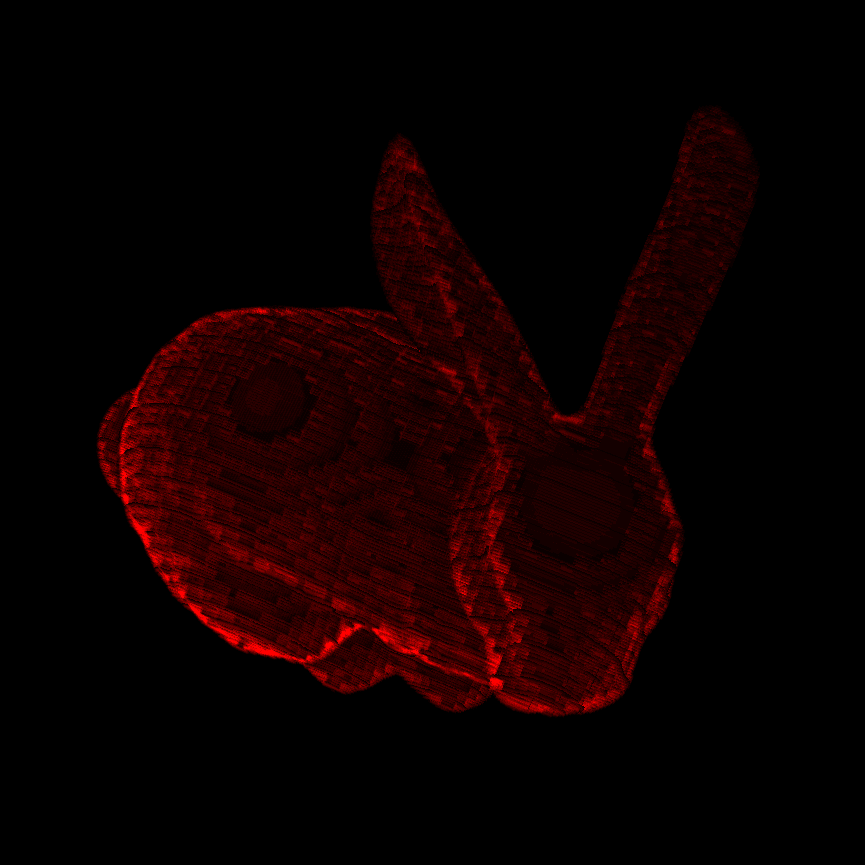
\includegraphics[width=100px]{images/graphics/overdraw-bunny2-pmoc.png}
    \caption{}
    \parbox{\linewidth}{\centering\footnotesize Per-Meshlet\\Occlusion Culling}
  \end{subfigure}
  \begin{subfigure}{100px}
    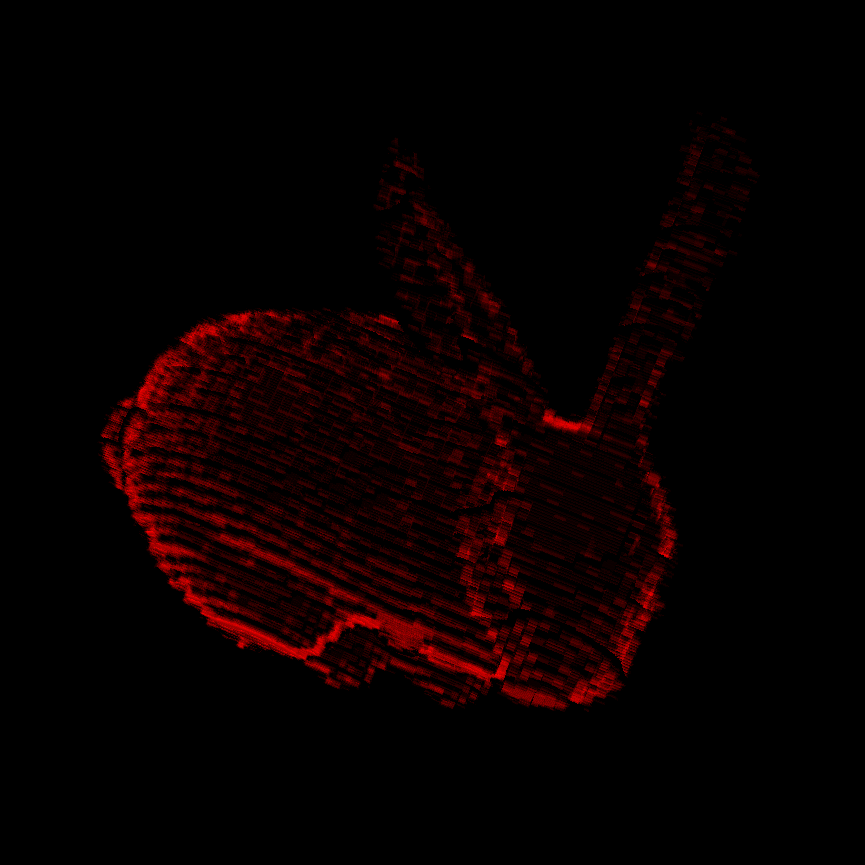
\includegraphics[width=100px]{images/graphics/overdraw-bunny2-diff.png}
    \caption{}
    \parbox{\linewidth}{\centering\footnotesize Difference\\(b) vs. (c)}
  \end{subfigure}

  \caption{Overdraw of the pixels from two different camera angles. 
  The image values are enhanced for better visualization.}
  \label{fig:bunny-overdraw}
\end{figure}

\noindent
Figure \ref{fig:bunny-overdraw} shows that the \ac{PONOC} had more overdrawn pixels than the 
\ac{PMOC} configuration. The difference is in favor of \ac{PMOC}, which had only a maximum of 
43 draws to the same pixels as compared to 60 draws. Without the culling activated, the maximum 
amount of overdraw was measured to be 111 draws to the same pixel. The camera angle clearly made 
a difference here, as the top view increased the amount of overdraw significantly. This is 
especially visible on the surface of the model, where a lot of rounded edges are present. \\

\noindent
The images also show how the \ac{PONOC} produces more overdraw on the surface than the \ac{PMOC} 
because a larger portion of the voxels on the outside of the mesh were being culled. In Figure 
\ref{fig:bunny-overdraw}, this is visible as the broad red outline around the bunny. The rightmost 
column additionally highlights a considerable difference in overdraw between the two occlusion 
culling configurations.

\clearpage



\subsection*{Torus}

The \emph{Torus} provides a high voxel count and has a hole in it, which creates an area where the 
octree isn't densely filled with voxels. This model was specifically intended to test the algorithm's 
capabilities of culling voxels in a scene that is densely crowded in some parts and provides areas with 
no voxels in other parts, i.e., the hole in the middle. Also, the \emph{Torus} is an inherently round 
shape and is therefore expected to have a lot of partially filled octree nodes representing its surface. 

\subsubsection*{Culling Results} \label{subsubsec-culling-results-torus}

% --------------------------------------- TORUS 256 --------------------------------------

\begin{figure}[!htb]              % Torus 256 Voxels Test Anim
    \begin{center}
      \begin{tikzpicture}
        \begin{axis}[
            width=\linewidth, % Scale the plot to \linewidth
            height=100px,
            xlabel={Frames},
            ylabel={Computed Voxels},
            grid,
            xmin=0,
            xmax=1087,
            ymin=70000,
            ymax=500000,
            legend style={at={(0.5,1.7)}, anchor=north, legend columns=2},
          ]
          \addplot[blue, no marks, solid] table[col sep=comma, x=frame, x expr=\thisrow{frame} * 1087 / 1087, y=visible_voxels]{./plotdata/torus_256_voxels.csv};
          \addplot[red, no marks, solid] table[col sep=comma, x=frame, x expr=\thisrow{frame} * 1087 / 1845, y=visible_voxels]{./plotdata/torus_256_voxels_pmoc.csv};
          \addplot[blue, dotted, no marks, domain=0:1087, samples=50] {359313};
          \addplot[red, dotted, no marks, domain=0:1087, samples=50] {170772};
          \legend{Per-Octree Occlsion Culling, Per-Meshlet Occlusion Culling}
        \end{axis}
      \end{tikzpicture}

      \begin{tikzpicture}
        \begin{axis}[
            width=\linewidth, % Scale the plot to \linewidth
            height=100px,
            xlabel={Frames},
            ylabel={Computed Nodes},
            grid,
            xmin=0,
            xmax=1087,
            ymin=1000,
            ymax=10000,
            legend style={at={(0.5,1.7)}, anchor=north, legend columns=2},
          ]
          \addplot[blue, no marks, solid] table[col sep=comma, x=frame, x expr=\thisrow{frame} * 1087 / 1087, y=visible_nodes]{./plotdata/torus_256_nodes.csv};
          \addplot[red, no marks, solid] table[col sep=comma, x=frame, x expr=\thisrow{frame} * 1087 / 1845, y=visible_nodes]{./plotdata/torus_256_nodes_pmoc.csv};
          \addplot[blue, dotted, no marks, domain=0:1087, samples=50] {7712};
          \addplot[red, dotted, no marks, domain=0:1087, samples=50] {4768};
          \legend{Per-Octree Occlsion Culling, Per-Meshlet Occlusion Culling}
        \end{axis}
      \end{tikzpicture}
    \end{center}

    \caption{\textbf{First:} The amount of visible voxels over the course of the test animation. \\
    \textbf{Second:} The amount of visible octree nodes over the course of the test animation.}
    \label{plt:torus-256-culling-res-voxels}
  \end{figure}

% ----------------------------------------------------------------------------------------

\noindent
As Figure \ref{plt:torus-256-culling-res-voxels} shows, the \emph{Torus} model varied in culling efficiency 
depending on the view angle. As expected, the hole in the mesh turned out to be inefficient for the culling 
algorithm. When considering the occlusion ratio, both the \ac{PONOC} and the \ac{PMOC} performed significantly 
better when the torus was viewed from an angle from which the hole in the middle was occluded. \\

\noindent
The average number of visible voxels was 359,313 for \ac{PONOC} and 170,772 for \ac{PMOC}, while the number 
of total voxels in the scene was 2,311,006. The average amount of visible octree nodes was 7,712 for \ac{PONOC} 
and 4,768 for \ac{PMOC}. The number of total octree nodes in the scene was 39,794. \\

\noindent
The data suggests that the \emph{Torus} was able to be used for both occlusion culling configurations and benefitted 
from the more granular \ac{PMOC} while still being considerably dependent on the viewing angle of the camera. The 
average culling ratio was $84.5\%$ for \ac{PONOC} and $92.6\%$ for \ac{PMOC}. For the former, the number of visible 
voxels diverged by a maximum of $56.05\%$ from the average value, while the latter diverged by a maximum of $50.74\%$. 
For the visible octree nodes, the variations were $52.11\%$ for \ac{PONOC} and $55.23\%$ for \ac{PMOC}.

\subsubsection*{CPU Performance Results} \label{subsubsec-cpu-performance-results-torus}

\begin{figure}[!htb]              % Torus CPU times
  \begin{center}
    \begin{tikzpicture}
      \begin{axis}[
          width=\linewidth,
          height=100px,
          xlabel={Frames},
          ylabel={Update Time (s)},
          grid,
          xmin=0,
          xmax=1087,
          ymin=0,
          ymax=0.00005,
          legend style={at={(0.5,1.8)}, anchor=north, legend columns=2},
        ]
        \addplot[brown!60, no marks, solid] table[col sep=comma, x=frame, x expr=\thisrow{frame} * 1087 / 1262, y=time]{./plotdata/cpu/torus_256_updateTime_nocull.csv};
        \addplot[blue, no marks, solid] table[col sep=comma, x=frame, x expr=\thisrow{frame} * 1554 / 1863, y=time]{./plotdata/cpu/torus_256_updateTime_pooc.csv};
        \addplot[red, no marks, solid] table[col sep=comma, x=frame, x expr=\thisrow{frame} * 1087 / 1785, y=time]{./plotdata/cpu/torus_256_updateTime.csv};
        \legend{No Occlusion Culling, Per-Octree Occlsion Culling, Per-Meshlet Occlusion Culling}
      \end{axis}
    \end{tikzpicture}
    \begin{tikzpicture}
      \begin{axis}[
          width=\linewidth,
          height=100px,
          xlabel={Frames},
          ylabel={Render Time (s)},
          grid,
          xmin=0,
          xmax=1087,
          ymin=0,
          ymax=0.00025,
          legend style={at={(0.5,1.8)}, anchor=north, legend columns=2},
        ]
        \addplot[brown!60, no marks, solid] table[col sep=comma, x=frame, x expr=\thisrow{frame} * 1087 / 1262, y=time]{./plotdata/cpu/torus_256_renderTime_nocull.csv};
        \addplot[blue, no marks, solid] table[col sep=comma, x=frame, x expr=\thisrow{frame} * 1087 / 1554, y=time]{./plotdata/cpu/torus_256_renderTime_pooc.csv};
        \addplot[red, no marks, solid] table[col sep=comma, x=frame, x expr=\thisrow{frame} * 1087 / 1785, y=time]{./plotdata/cpu/torus_256_renderTime.csv};
        \legend{No Occlusion Culling, Per-Octree Occlsion Culling, Per-Meshlet Occlusion Culling}
      \end{axis}
    \end{tikzpicture}
  \end{center}
  \caption{Overview of the render times over the course of the test animation. The upper graph shows the time 
  each frame took to execute the \emph{Update()} function on the \ac{CPU}. The lower graph shows the time each 
  frame took to execute the function \emph{Render()} on the \ac{CPU}. This includes the completion of the 
  \ac{GPU} computations.}
  \label{plt:torus-256-culling-cpu-time}
\end{figure}

\noindent
Figure \ref{plt:torus-256-culling-cpu-time} shows that the \emph{Torus} showed very similar \ac{CPU} performances 
in both occlusion culling configurations. The measurements show small differences for the \emph{Render()} function 
when comparing the base pipeline to the occlusion culling pipelines. The difference was only present in the first 300 
frames of the animation, and it cannot be reliably attributed to any particular difference in the occlusion culling 
algorithm. Comparing the \ac{PONOC} to the \ac{PMOC}, there are similar differences, which only occurred during a 
short time of the test animation. Because these differences were not measurable over the whole test, both pipelines 
are considered to be similar in \ac{CPU} time.

\subsubsection*{GPU Performance Results} \label{subsubsec-gpu-performance-results-torus}

\begin{figure}[!htb]              % Torus GPU times
  \centering
  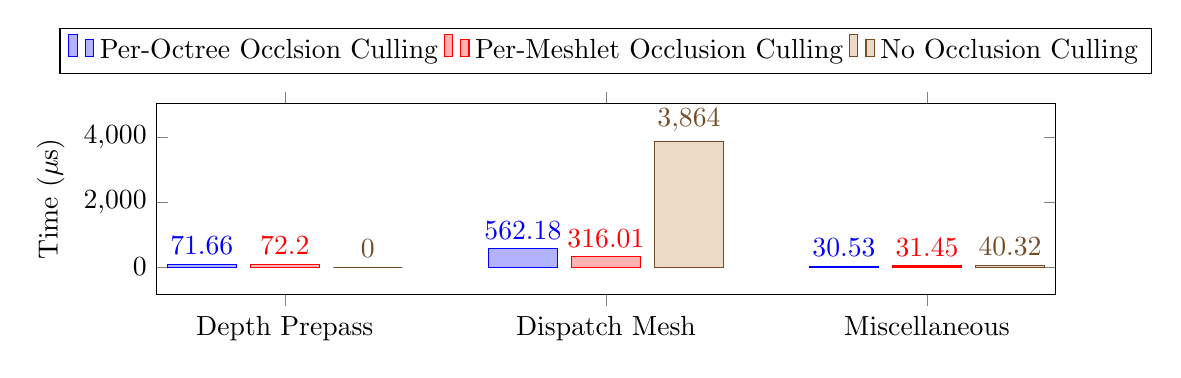
\begin{tikzpicture}
    \begin{axis}[
        height=4cm,
        width=13cm,
        x tick label style={/pgf/number format/1000 sep=},
        ylabel={Time ($\mu$s)},
        legend style={at={(0.5,1.4)}, anchor=north, legend columns=-1},
        symbolic x coords={DepthPrepass, DispatchMesh, Misc},
        xticklabels={Depth Prepass, Dispatch Mesh, Miscellaneous},
        xtick=data,
        ybar=0.4,
        bar width=25pt,
        ymin=0,
        ymax=4200,
        nodes near coords,
        enlargelimits=0.2,
    ]
    \addplot+[bar shift=-30pt] coordinates {(DepthPrepass,71.66) (DispatchMesh,562.18) (Misc,30.53)};
    \addplot+[bar shift=0pt] coordinates {(DepthPrepass,72.20) (DispatchMesh,316.01) (Misc,31.4482)};
    \addplot+[bar shift=30pt] coordinates {(DepthPrepass,0) (DispatchMesh,3864.0) (Misc,40.31696)};
    \legend{Per-Octree Occlsion Culling, Per-Meshlet Occlusion Culling, No Occlusion Culling}
    \end{axis}
  \end{tikzpicture}

  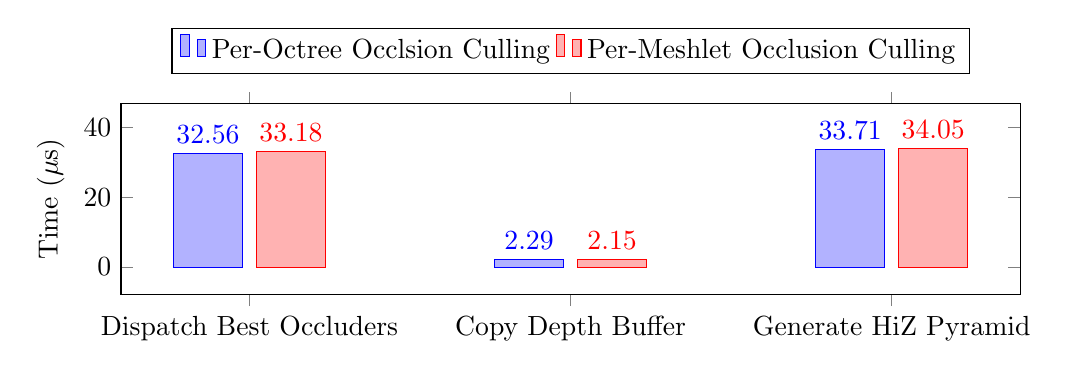
\begin{tikzpicture}
    \begin{axis}[
        height=4cm,
        width=13cm,
        x tick label style={/pgf/number format/1000 sep=},
        ylabel={Time ($\mu$s)},
        legend style={at={(0.5,1.4)}, anchor=north, legend columns=-1},
        symbolic x coords={DispatchBestOccluders, CopyTex, GenMipChain},
        xticklabels={Dispatch Best Occluders, Copy Depth Buffer, Generate \ac{HiZ} Pyramid},
        xtick=data,
        ybar=0.4,
        bar width=25pt,
        ymin=0,
        ymax=39,
        nodes near coords,
        enlargelimits=0.2,
    ]
    \addplot+[bar shift=-15pt] coordinates {(DispatchBestOccluders,32.56) (CopyTex,2.29) (GenMipChain,33.71)};
    \addplot+[bar shift=15pt] coordinates {(DispatchBestOccluders,33.18) (CopyTex,2.15) (GenMipChain,34.05)};
    \legend{Per-Octree Occlsion Culling, Per-Meshlet Occlusion Culling}
    \end{axis}
  \end{tikzpicture}
  \caption{\textbf{First:} The complete time measured on the \ac{GPU}. The \emph{Depth Prepass} is the extra 
  overhead introduced by the \ac{HZB}. The \emph{Dispatch Mesh} is the drawing of the meshes, including the 
  occlusion culling. \emph{Miscellaneous} includes a small amount of \emph{Barriers} used for synchronization 
  and the rendering of some debug \ac{UI}. It is considered to be more or less static in computation time and 
  is not part of the actual algorithm measured in this experiment. \textbf{Second:} The time measured in the 
  \emph{Depth Prepass}. The \emph{Dispatch Best Occluders} is the drawing to the depth buffer. The 
  \emph{Copy Depth Buffer} computation copies the depth buffers content into the final \ac{HiZ} resource. Finally, 
  \emph{Generate HiZ Pyramid} shows the \ac{HiZ} creation, which is done sequentially.}
  \label{fig:torus-gpu-results}
\end{figure}

\noindent
The \ac{GPU} performance for the \emph{Torus} model was considerably better using the \ac{PMOC} approach. 
While the depth prepass differed by only 0.54 microseconds in favor of the \ac{PONOC}, the complete time 
spent on the \ac{GPU} was decreased by $36.8\%$ using the \ac{PMOC} configuration as shown in Figure 
\ref{fig:torus-gpu-results}. \\

\noindent
Both culling configurations decreased the time spent on the \ac{GPU} compared to the base pipeline by 
$83.0\%$ and $89.3\%$, respectively.

\subsubsection*{Overdraw}

\begin{figure}[!htbp]
  \centering
  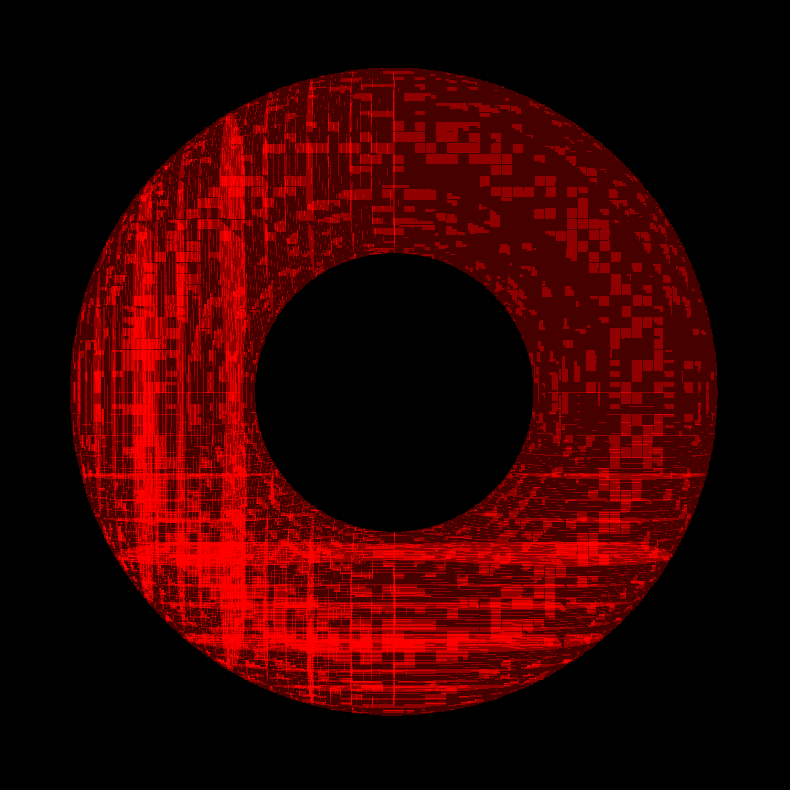
\includegraphics[height=100px]{images/graphics/overdraw-torus1-nocull.png}
  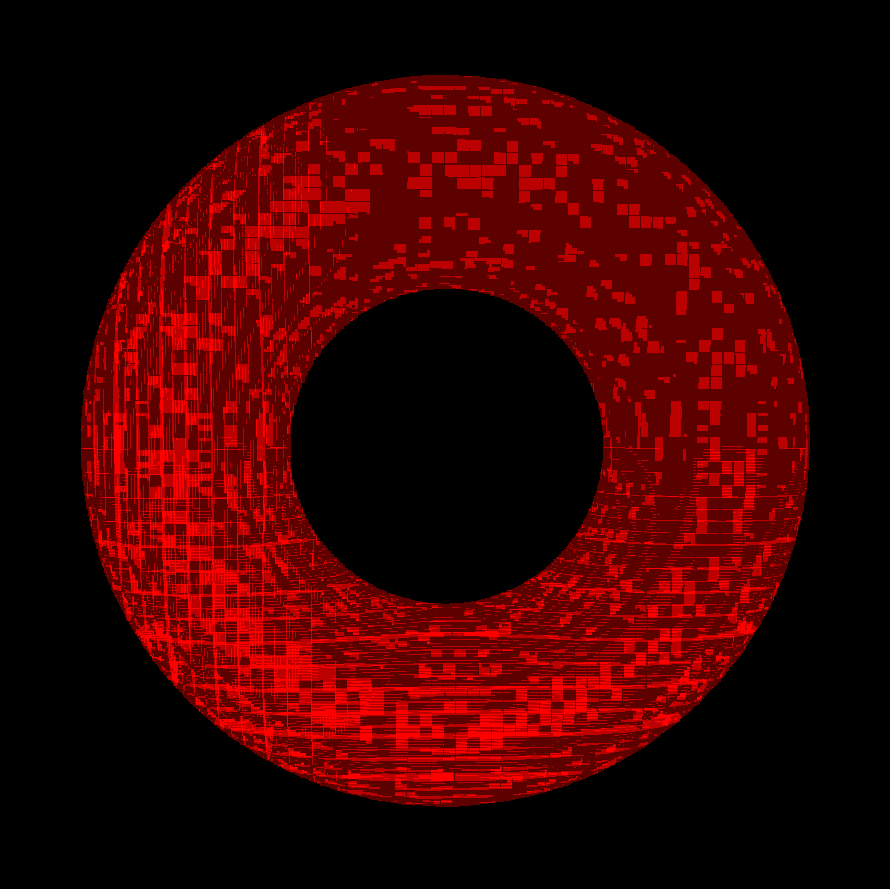
\includegraphics[height=100px]{images/graphics/overdraw-torus1-pooc.png}
  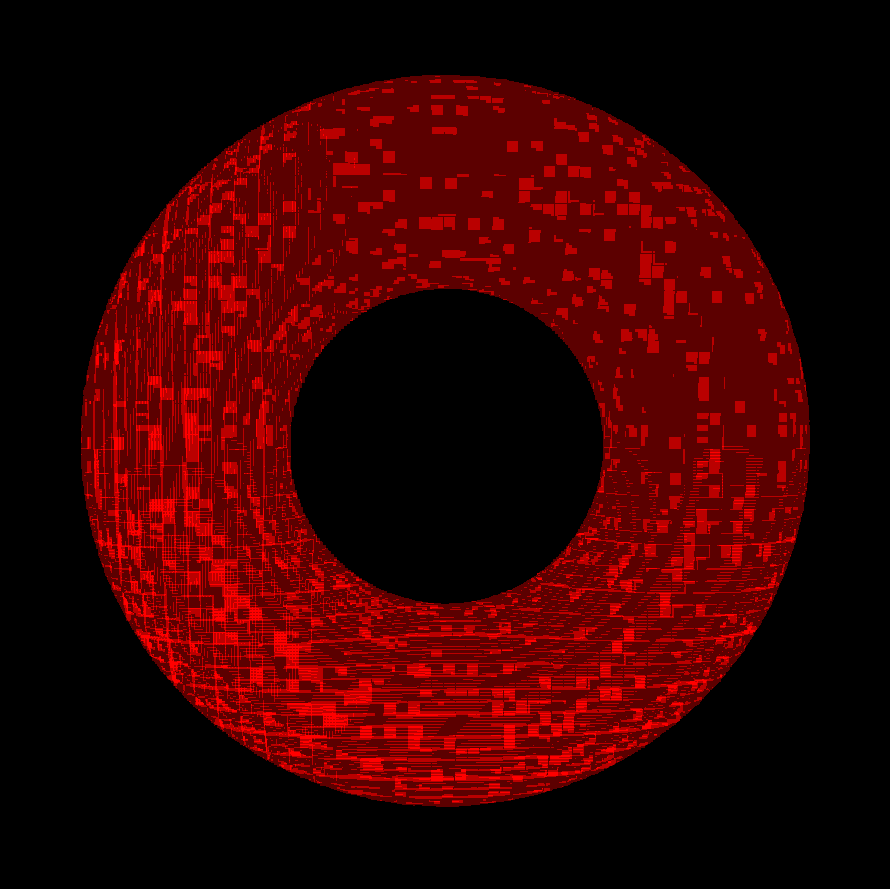
\includegraphics[height=100px]{images/graphics/overdraw-torus1-pmoc.png}
  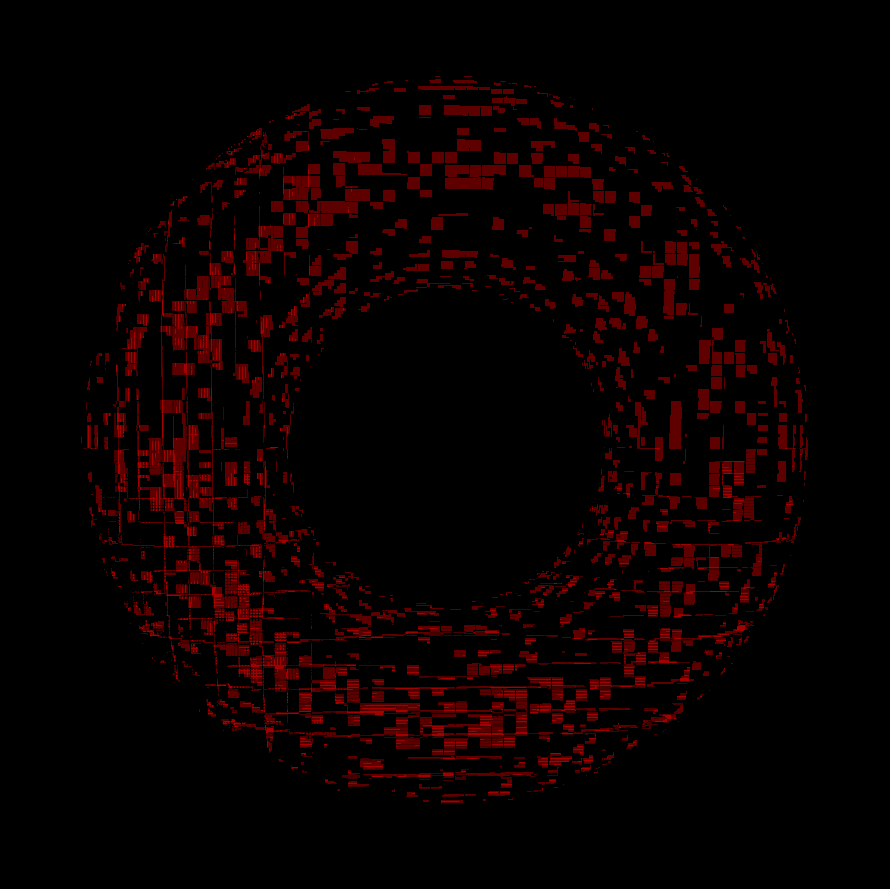
\includegraphics[height=100px]{images/graphics/overdraw-torus1-diff.png}

  \begin{subfigure}{100px}
    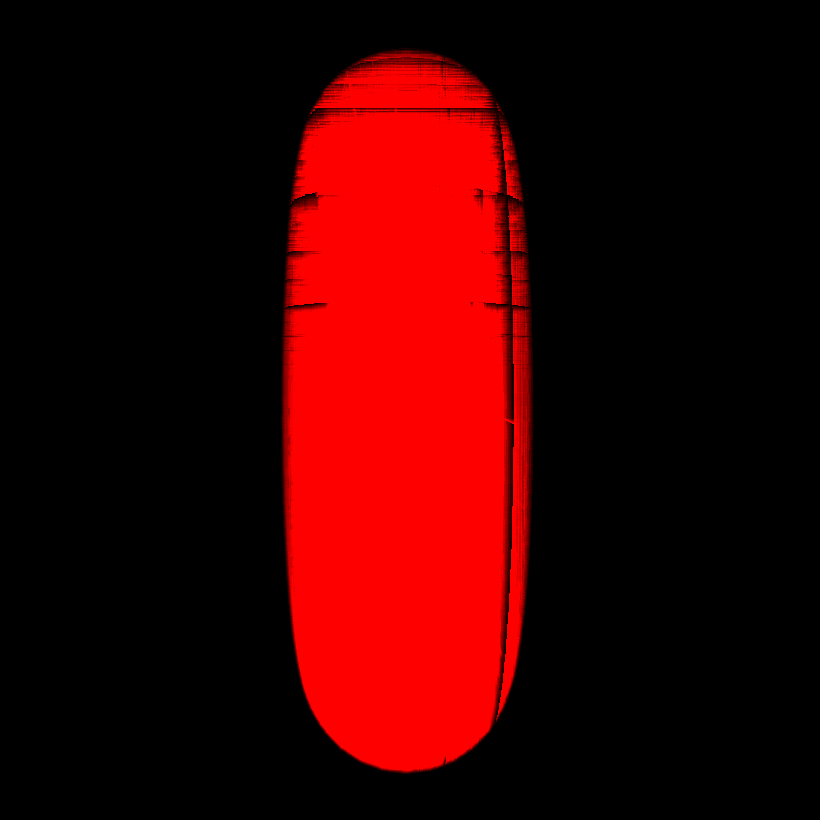
\includegraphics[height=100px]{images/graphics/overdraw-torus2-nocull.png}
    \caption{}
    \parbox{\linewidth}{\centering\footnotesize No Occlusion\\Culling}
  \end{subfigure}
  \begin{subfigure}{100px}
    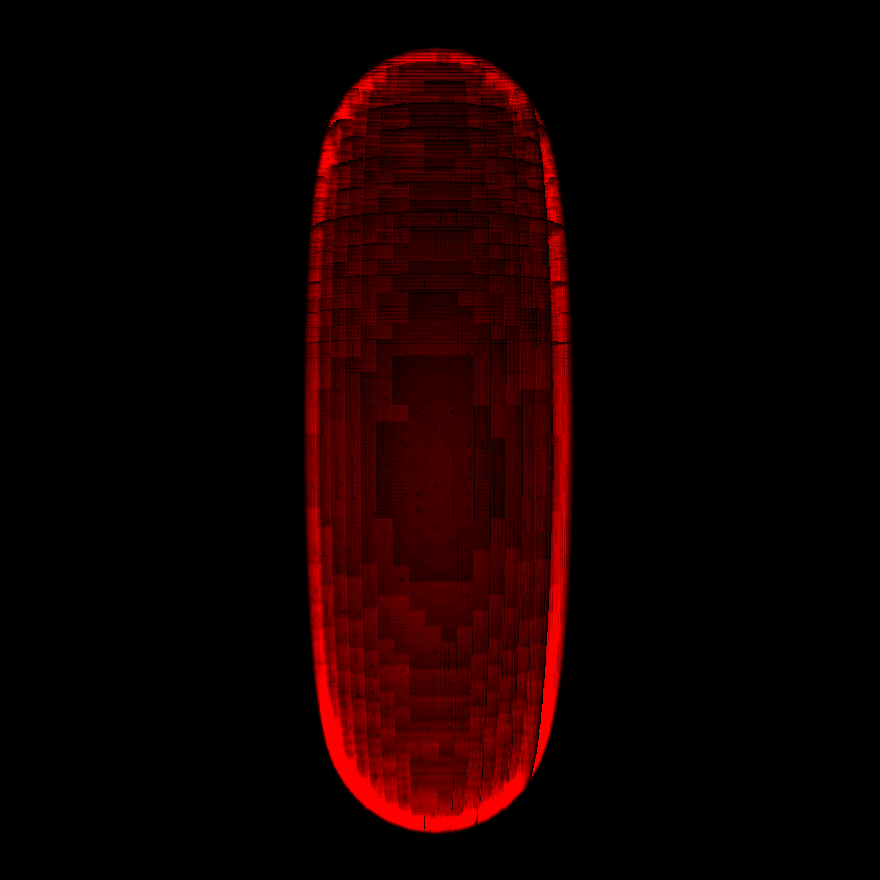
\includegraphics[height=100px]{images/graphics/overdraw-torus2-pooc.png}
    \caption{}
    \parbox{\linewidth}{\centering\footnotesize Per-Octree Node\\Occlusion Culling}
  \end{subfigure}
  \begin{subfigure}{100px}
    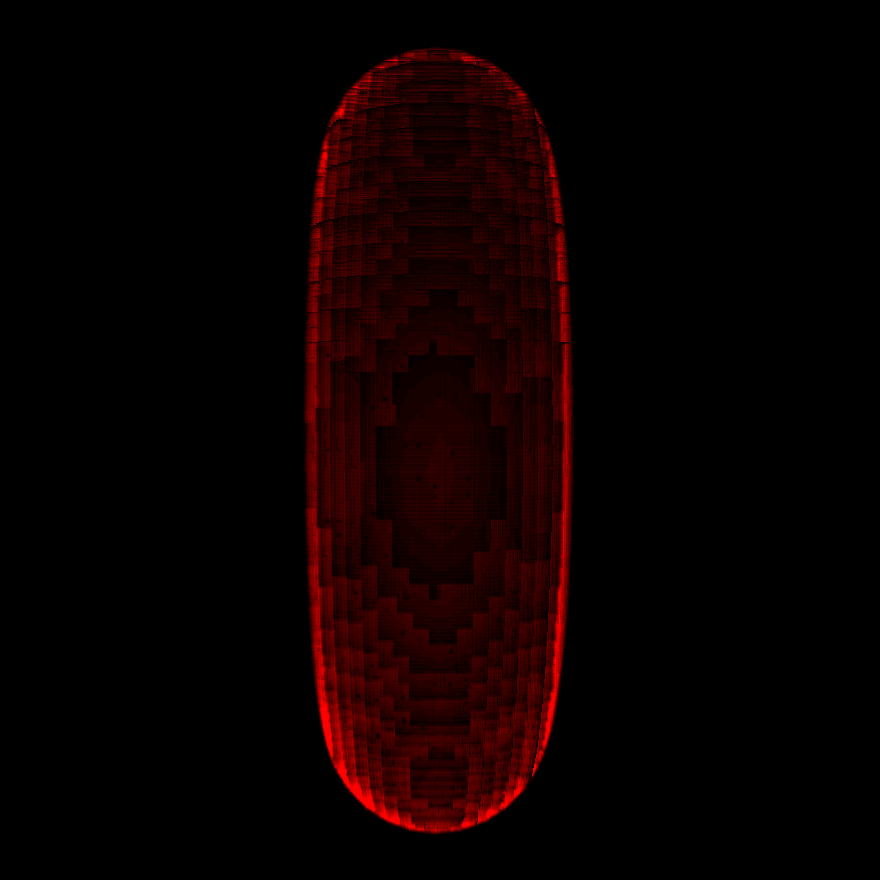
\includegraphics[height=100px]{images/graphics/overdraw-torus2-pmoc.png}
    \caption{}
    \parbox{\linewidth}{\centering\footnotesize Per-Meshlet\\Occlusion Culling}
  \end{subfigure}
  \begin{subfigure}{100px}
    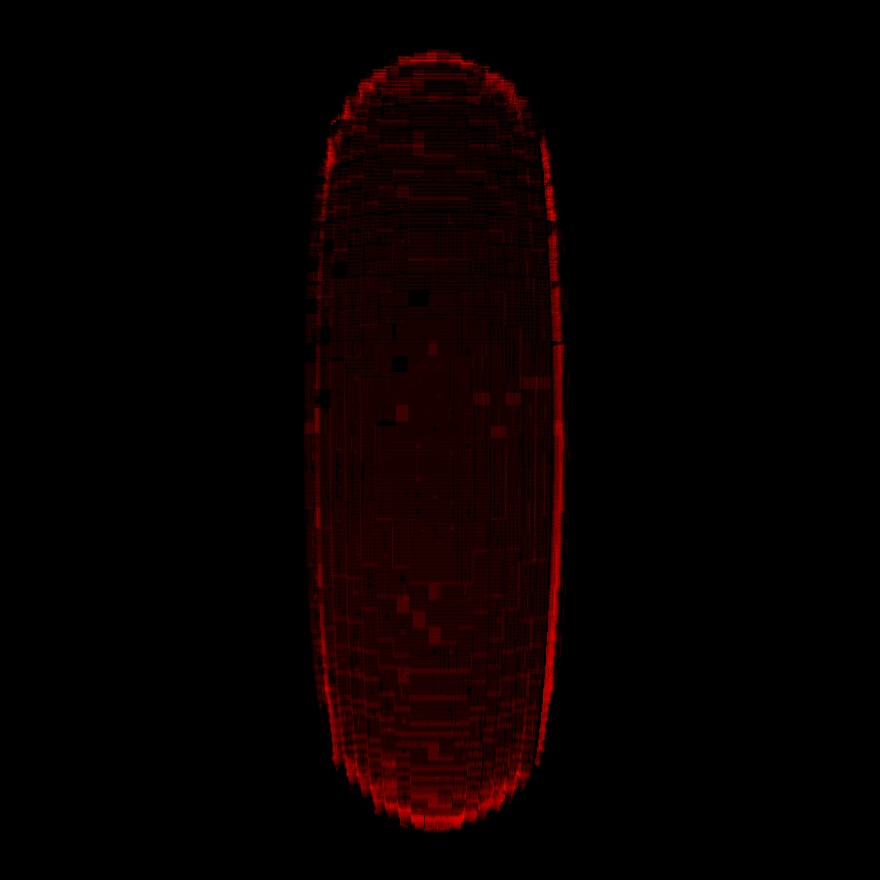
\includegraphics[height=100px]{images/graphics/overdraw-torus2-diff.png}
    \caption{}
    \parbox{\linewidth}{\centering\footnotesize Difference\\(b) vs. (c)}
  \end{subfigure}

  \caption{Overdraw of the pixels from two different camera angles. 
  The image values are enhanced for better visualization.}
  \label{fig:torus-overdraw}
\end{figure}

\noindent
Figure \ref{fig:torus-overdraw} shows the overdraw for the \emph{Torus} model from two 
camera perspectives. Clearly, the \ac{PMOC} configuration resulted in less overdraw, 
especially when viewed from the sides. As the second row of figure \ref{fig:torus-overdraw} 
shows, the edges were particularly overdrawn because of the missing depth information. 
Without culling, the maximum amount of overdraw was measured to be 267 draws to one pixel.


\clearpage



\subsection*{Terrain}

The \emph{Terrain} model aimed to replicate a relatively flat, open area that could be found in actual 
games like \emph{Minecraft} (Mojang \cite{Mojang2024}, 2011). Its surface is set up in a way that allows 
for only a small layer of the best occluders to be formed. The terrain's hills are assumed to be occluding 
a large part of the scene, which would help for rendering such a scene in a game.

\subsubsection*{Culling Results} \label{subsubsec-culling-results-terrain}

% -------------------------------------- TERRAIN 256 -------------------------------------

\begin{figure}[!htb]              % Terrain 256 Voxels Test Anim
    \begin{center}
      \begin{tikzpicture}
        \begin{axis}[
            width=\linewidth, % Scale the plot to \linewidth
            height=100px,
            xlabel={Frames},
            ylabel={Computed Voxels},
            grid,
            xmin=0,
            xmax=1239,
            ymin=70000,
            ymax=500000,
            legend style={at={(0.5,1.7)}, anchor=north, legend columns=2},
          ]
          \addplot[blue, no marks, solid] table[col sep=comma, x=frame, x expr=\thisrow{frame} * 1239 / 1239, y=visible_voxels]{./plotdata/terrain_256_voxels.csv};
          \addplot[red, no marks, solid] table[col sep=comma, x=frame, x expr=\thisrow{frame} * 1239 / 1759, y=visible_voxels]{./plotdata/terrain_256_voxels_pmoc.csv};
          \addplot[blue, dotted, no marks, domain=0:1239, samples=50] {396228};
          \addplot[red, dotted, no marks, domain=0:1239, samples=50] {180440};
          \legend{Per-Octree Occlsion Culling, Per-Meshlet Occlusion Culling}

        \end{axis}
      \end{tikzpicture}

      \begin{tikzpicture}
        \begin{axis}[
            width=\linewidth, % Scale the plot to \linewidth
            height=100px,
            xlabel={Frames},
            ylabel={Computed Nodes},
            grid,
            xmin=0,
            xmax=1239,
            ymin=2000,
            ymax=10000,
            legend style={at={(0.5,1.7)}, anchor=north, legend columns=2},
          ]
          \addplot[blue, no marks, solid] table[col sep=comma, x=frame, x expr=\thisrow{frame} * 1239 / 1239, y=visible_nodes]{./plotdata/terrain_256_nodes.csv};
          \addplot[red, no marks, solid] table[col sep=comma, x=frame, x expr=\thisrow{frame} * 1239 / 1759, y=visible_nodes]{./plotdata/terrain_256_nodes_pmoc.csv};
          \addplot[blue, dotted, no marks, domain=0:1239, samples=50] {8207};
          \addplot[red, dotted, no marks, domain=0:1239, samples=50] {3832};
          \legend{Per-Octree Occlsion Culling, Per-Meshlet Occlusion Culling}

        \end{axis}
      \end{tikzpicture}

      \caption{\textbf{First:} The amount of visible voxels over the course of the test animation. \\
      \textbf{Second:} The amount of visible octree nodes over the course of the test animation.}
      \label{plt:terrain-256-culling-res-voxels}
    \end{center}
  \end{figure}

% ----------------------------------------------------------------------------------------

\noindent
The \emph{Terrain} model showed a rather stable occlusion over time. For this scene, it was essential that the 
model in question had a minimal volume to it so the best occluders could be found and computed. \\

\noindent
The average number of visible voxels was 396,228 for \ac{PONOC} and 180,440 for \ac{PMOC}, while the number of total 
voxels in the scene was 953,362. The average amount of visible octree nodes was 8,207 for \ac{PONOC} and 3,832 for 
\ac{PMOC}. The number of total octree nodes in the scene was 18,465. \\

\noindent
The data suggests that the \emph{Terrain} was able to be used for both occlusion culling configurations and benefitted from 
the more granular \ac{PMOC} while still being considerably dependent on the viewing angle of the camera. The average 
culling ratio was $58.4\%$ for \ac{PONOC} and $81.1\%$ for \ac{PMOC}. For the former, the number of visible voxels 
diverged by a maximum of $20.50\%$ from the average value, while the latter diverged by a maximum of $20.36\%$. 
For the visible octree nodes, the variations were $16.80\%$ for \ac{PONOC} and $17.12\%$ for \ac{PMOC}.

\subsubsection*{CPU Performance Results} \label{subsubsec-cpu-performance-results-terrain}

Figure \ref{plt:terrain-256-culling-cpu-time} shows the \ac{CPU} performance over time, which in general 
was similar for all tested pipeline configurations. Some parts of the test showed varying \ac{CPU} times, 
but this could not be reliably attributed to any of the differences in the measured algorithm. 

\begin{figure}[!htb]              % Terrain CPU times
  \begin{center}
    \begin{tikzpicture}
      \begin{axis}[
          width=\linewidth,
          height=100px,
          xlabel={Frames},
          ylabel={Update Time (s)},
          grid,
          xmin=0,
          xmax=1239,
          ymin=0,
          ymax=0.00005,
          legend style={at={(0.5,1.8)}, anchor=north, legend columns=2},
        ]
        \addplot[brown!60, no marks, solid] table[col sep=comma, x=frame, x expr=\thisrow{frame} * 1239 / 1381, y=time]{./plotdata/cpu/terrain_256_updateTime_nocull.csv};
        \addplot[blue, no marks, solid] table[col sep=comma, x=frame, x expr=\thisrow{frame} * 1239 / 1572, y=time]{./plotdata/cpu/terrain_256_updateTime_pooc.csv};
        \addplot[red, no marks, solid] table[col sep=comma, x=frame, x expr=\thisrow{frame} * 1239 / 1813, y=time]{./plotdata/cpu/terrain_256_updateTime.csv};
        \legend{No Occlusion Culling, Per-Octree Occlsion Culling, Per-Meshlet Occlusion Culling}
      \end{axis}
    \end{tikzpicture}
    \begin{tikzpicture}
      \begin{axis}[
          width=\linewidth,
          height=100px,
          xlabel={Frames},
          ylabel={Render Time (s)},
          grid,
          xmin=0,
          xmax=1239,
          ymin=0,
          ymax=0.00025,
          legend style={at={(0.5,1.8)}, anchor=north, legend columns=2},
        ]
        \addplot[brown!60, no marks, solid] table[col sep=comma, x=frame, x expr=\thisrow{frame} * 1239 / 1381, y=time]{./plotdata/cpu/terrain_256_renderTime_nocull.csv};
        \addplot[blue, no marks, solid] table[col sep=comma, x=frame, x expr=\thisrow{frame} * 1239 / 1572, y=time]{./plotdata/cpu/terrain_256_renderTime_pooc.csv};
        \addplot[red, no marks, solid] table[col sep=comma, x=frame, x expr=\thisrow{frame} * 1239 / 1813, y=time]{./plotdata/cpu/terrain_256_renderTime.csv};
        \legend{No Occlusion Culling, Per-Octree Occlsion Culling, Per-Meshlet Occlusion Culling}
      \end{axis}
    \end{tikzpicture}
    \caption{Overview of the render times over the course of the test animation. The upper graph shows the time 
    each frame took to execute the \emph{Update()} function on the \ac{CPU}. The lower graph shows the time each 
    frame took to execute the function \emph{Render()} on the \ac{CPU}. This includes the completion of the 
    \ac{GPU} computations.}
    \label{plt:terrain-256-culling-cpu-time}
  \end{center}
\end{figure}

\subsubsection*{GPU Performance Results} \label{subsubsec-gpu-performance-results-terrain}

Figure \ref{fig:terrain-gpu-times} shows the time spent on the \ac{GPU} for the \emph{Terrain} scene.
The complete time spent on the \ac{GPU} was decreased by $55.4\%$ using the \ac{PONOC} and by 
$74.1\%$ using the \ac{PMOC} as compared to the base pipeline without occlusion culling. The depth 
prepass didn't change significantly between both culling configurations. \\


\begin{figure}[!htb]
  \centering
  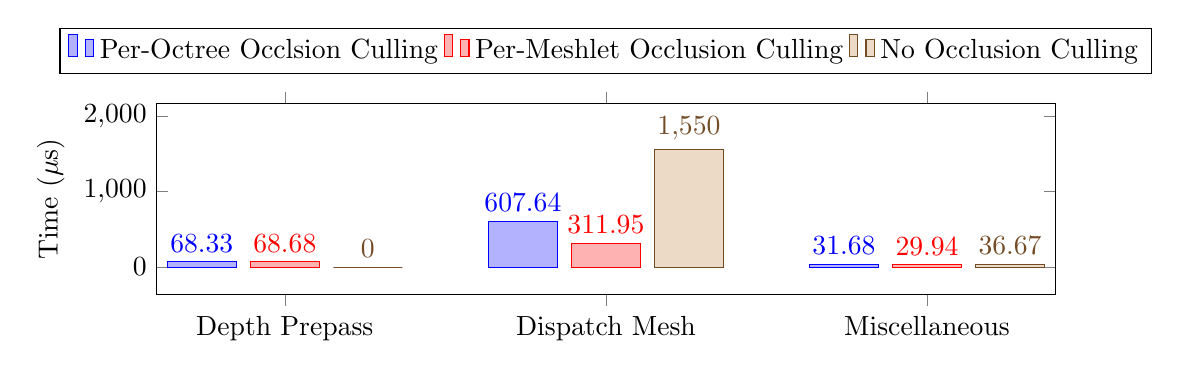
\begin{tikzpicture}
    \begin{axis}[
        height=4cm,
        width=13cm,
        x tick label style={/pgf/number format/1000 sep=},
        ylabel={Time ($\mu$s)},
        legend style={at={(0.5,1.4)}, anchor=north, legend columns=-1},
        symbolic x coords={DepthPrepass, DispatchMesh, Misc},
        xticklabels={Depth Prepass, Dispatch Mesh, Miscellaneous},
        xtick=data,
        ybar=0.4,
        bar width=25pt,
        ymin=0,
        ymax=1800,
        nodes near coords,
        enlargelimits=0.2,
    ]
    \addplot+[bar shift=-30pt] coordinates {(DepthPrepass,68.33) (DispatchMesh,607.64) (Misc,31.68)};
    \addplot+[bar shift=0pt] coordinates {(DepthPrepass,68.68) (DispatchMesh,311.95) (Misc,29.9444)};
    \addplot+[bar shift=30pt] coordinates {(DepthPrepass,0) (DispatchMesh,1550.00) (Misc,36.6748)};
    \legend{Per-Octree Occlsion Culling, Per-Meshlet Occlusion Culling, No Occlusion Culling}
    \end{axis}
  \end{tikzpicture}

  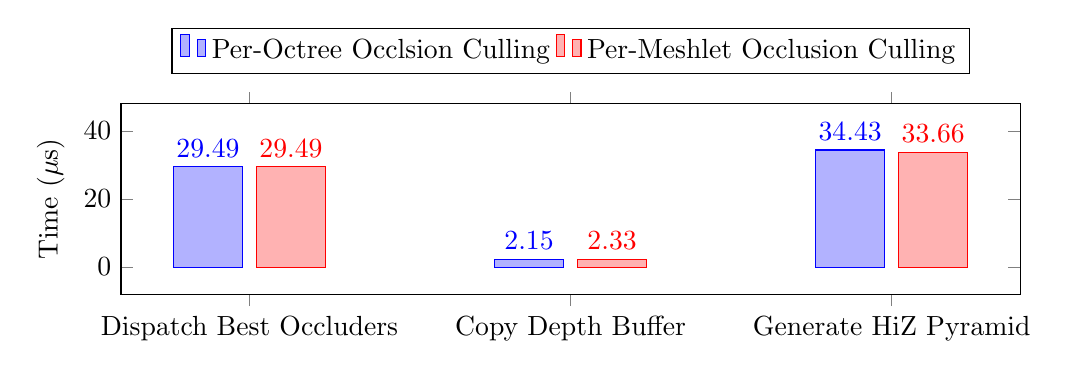
\begin{tikzpicture}
    \begin{axis}[
        height=4cm,
        width=13cm,
        x tick label style={/pgf/number format/1000 sep=},
        ylabel={Time ($\mu$s)},
        legend style={at={(0.5,1.4)}, anchor=north, legend columns=-1},
        symbolic x coords={DispatchBestOccluders, CopyTex, GenMipChain},
        xticklabels={Dispatch Best Occluders, Copy Depth Buffer, Generate \ac{HiZ} Pyramid},
        xtick=data,
        ybar=0.4,
        bar width=25pt,
        ymin=0,
        ymax=40,
        nodes near coords,
        enlargelimits=0.2,
    ]
    \addplot+[bar shift=-15pt] coordinates {(DispatchBestOccluders,29.49) (CopyTex,2.15) (GenMipChain,34.43)};
    \addplot+[bar shift=15pt] coordinates {(DispatchBestOccluders,29.49) (CopyTex,2.33) (GenMipChain,33.66)};
    \legend{Per-Octree Occlsion Culling, Per-Meshlet Occlusion Culling}
    \end{axis}
  \end{tikzpicture}
  \caption{\textbf{First:} The complete time measured on the \ac{GPU}. The \emph{Depth Prepass} is the extra 
  overhead introduced by the \ac{HZB}. The \emph{Dispatch Mesh} is the drawing of the meshes, including the 
  occlusion culling. \emph{Miscellaneous} includes a small amount of \emph{Barriers} used for synchronization 
  and the rendering of some debug \ac{UI}. It is considered to be more or less static in computation time and 
  is not part of the actual algorithm measured in this experiment. \textbf{Second:} The time measured in the 
  \emph{Depth Prepass}. The \emph{Dispatch Best Occluders} is the drawing to the depth buffer. The 
  \emph{Copy Depth Buffer} computation copies the depth buffers content into the final \ac{HiZ} resource. 
  Finally, \emph{Generate HiZ Pyramid} shows the \ac{HiZ} creation, which is done sequentially.}
  \label{fig:terrain-gpu-times}
\end{figure}

\subsubsection*{Overdraw}

\begin{figure}[!htb]
  \centering
  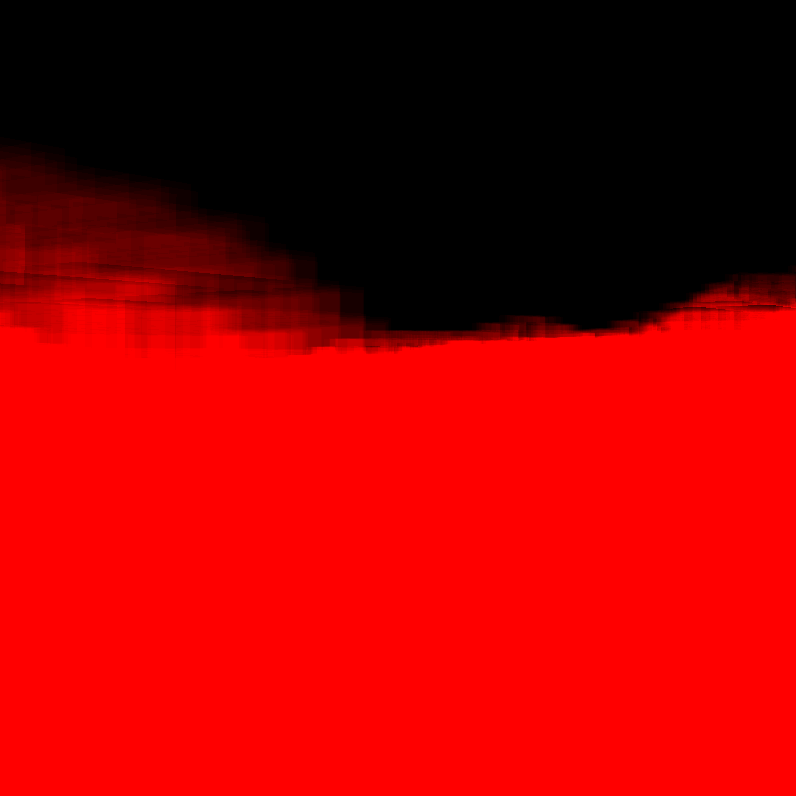
\includegraphics[height=100px]{images/graphics/overdraw-terrain1-nocull.png}
  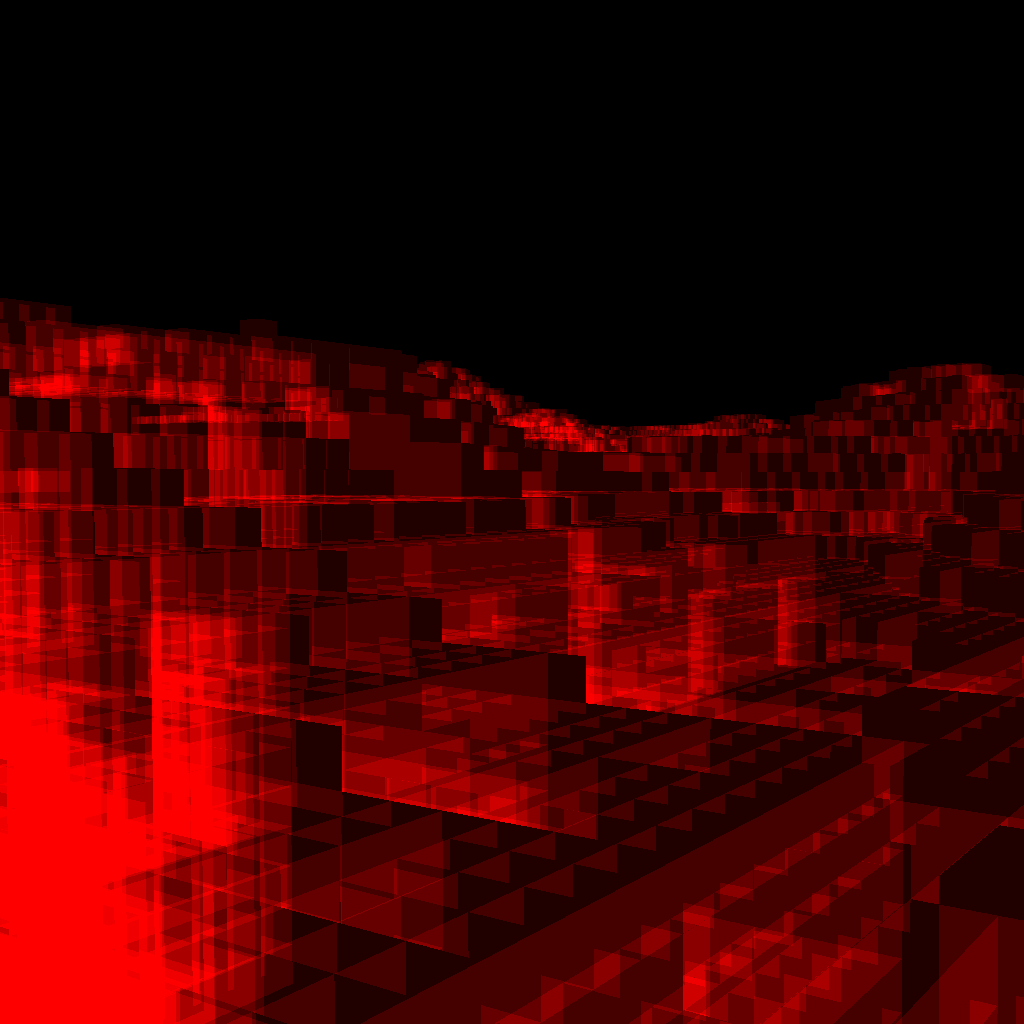
\includegraphics[height=100px]{images/graphics/overdraw-terrain1-pooc.png}
  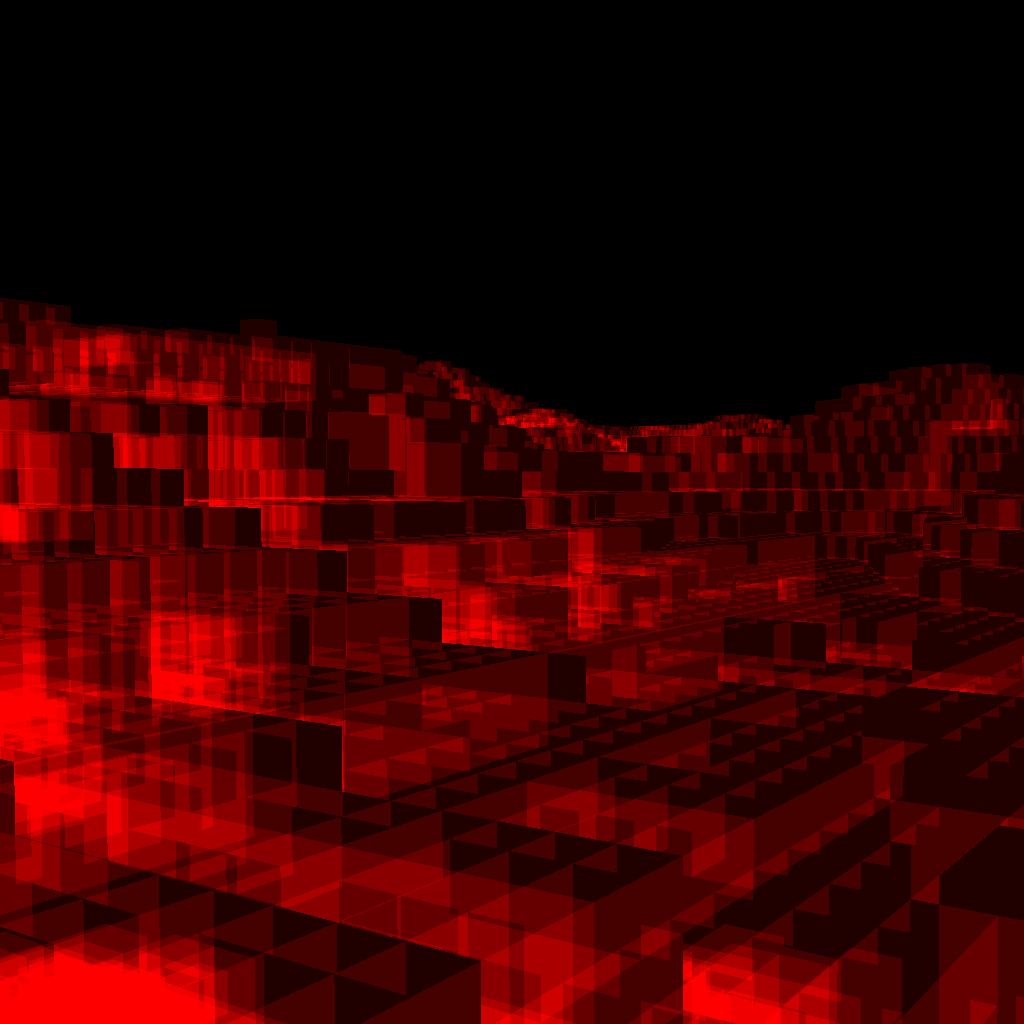
\includegraphics[height=100px]{images/graphics/overdraw-terrain1-pmoc.png}
  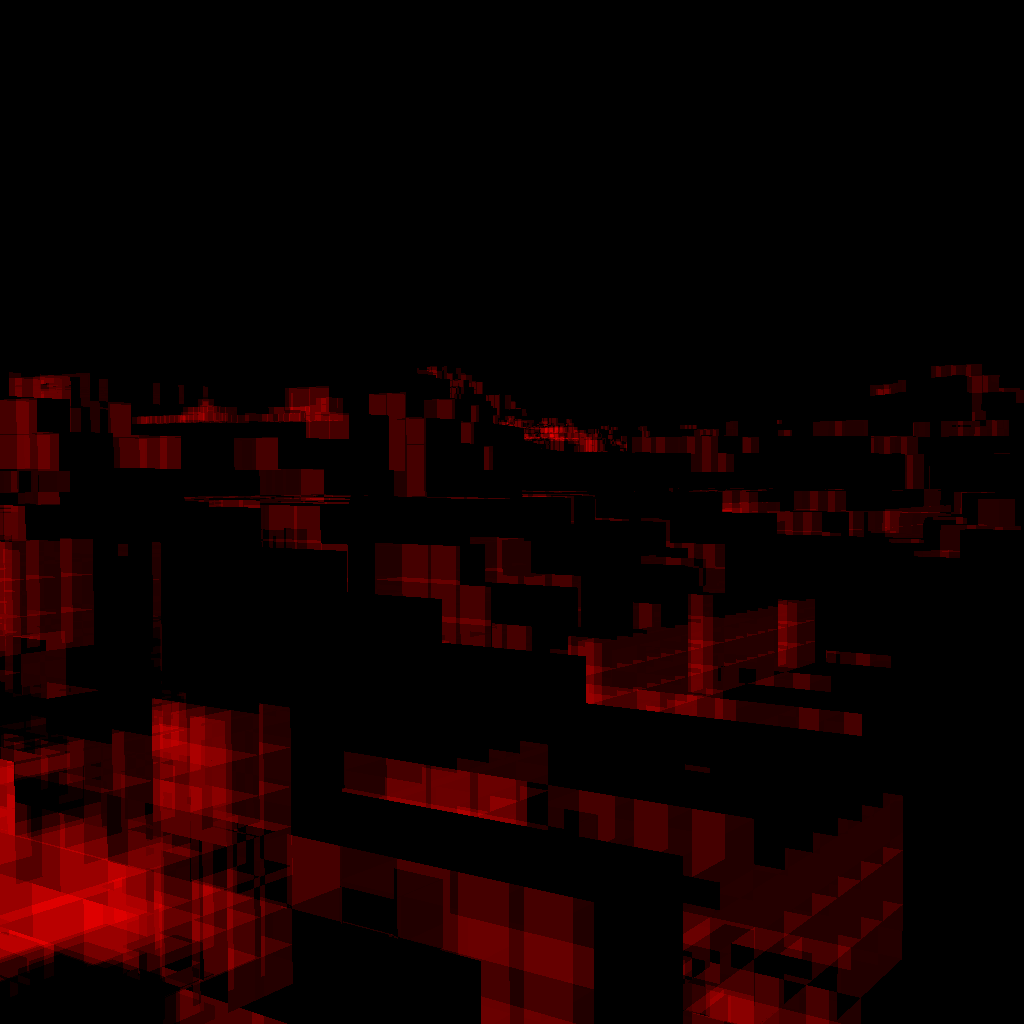
\includegraphics[height=100px]{images/graphics/overdraw-terrain1-diff.png}

  \begin{subfigure}{100px}
    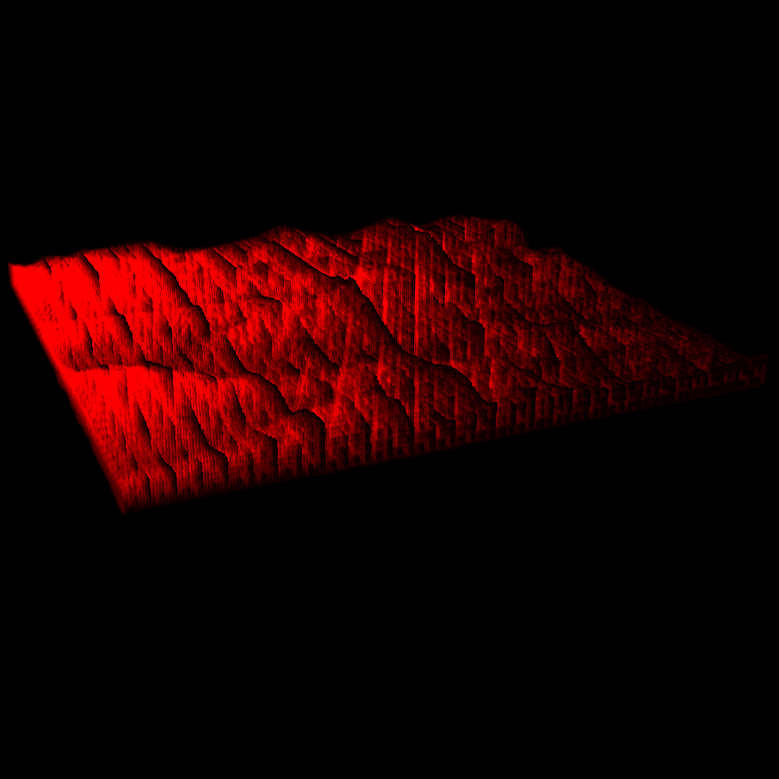
\includegraphics[height=100px]{images/graphics/overdraw-terrain2-nocull.png}
    \caption{}
    \parbox{\linewidth}{\centering\footnotesize No Occlusion\\Culling}
  \end{subfigure}
  \begin{subfigure}{100px}
    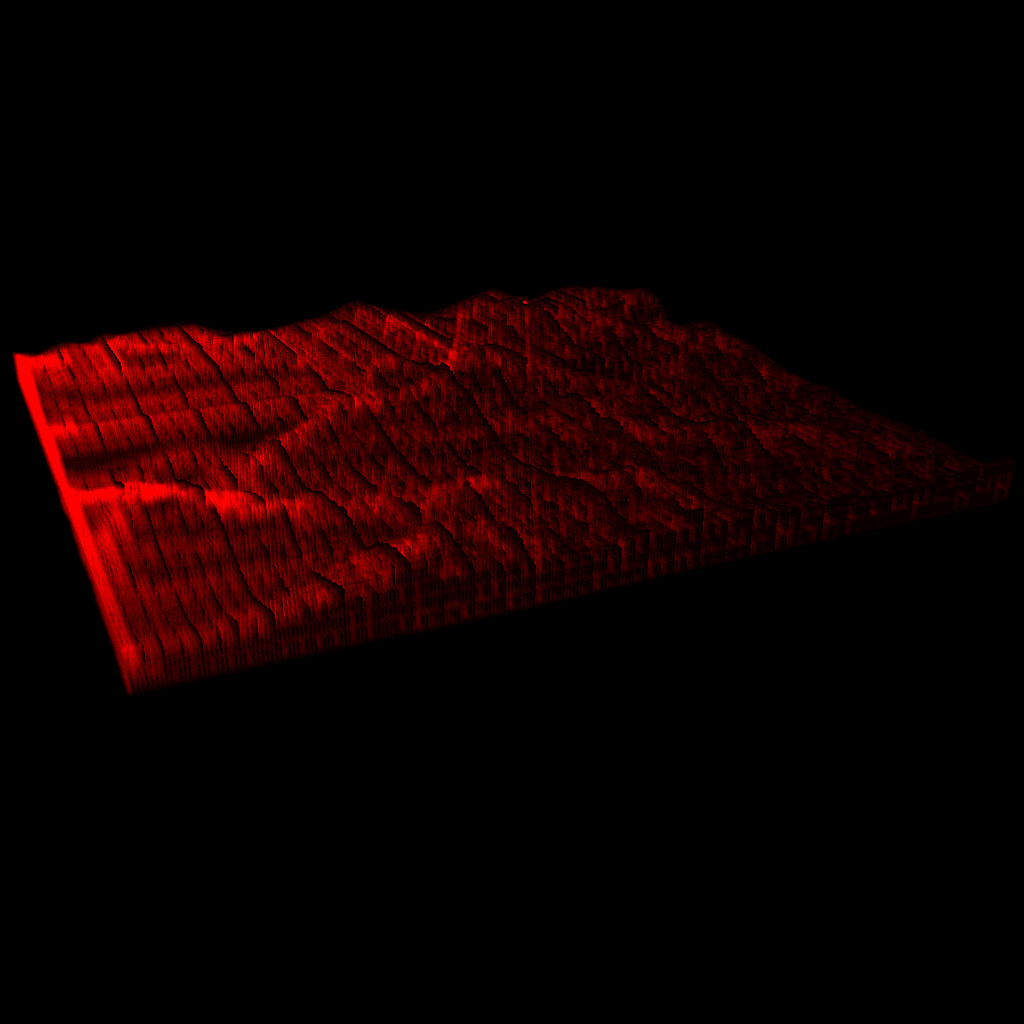
\includegraphics[height=100px]{images/graphics/overdraw-terrain2-pooc.png}
    \caption{}
    \parbox{\linewidth}{\centering\footnotesize Per-Octree Node\\Occlusion Culling}
  \end{subfigure}
  \begin{subfigure}{100px}
    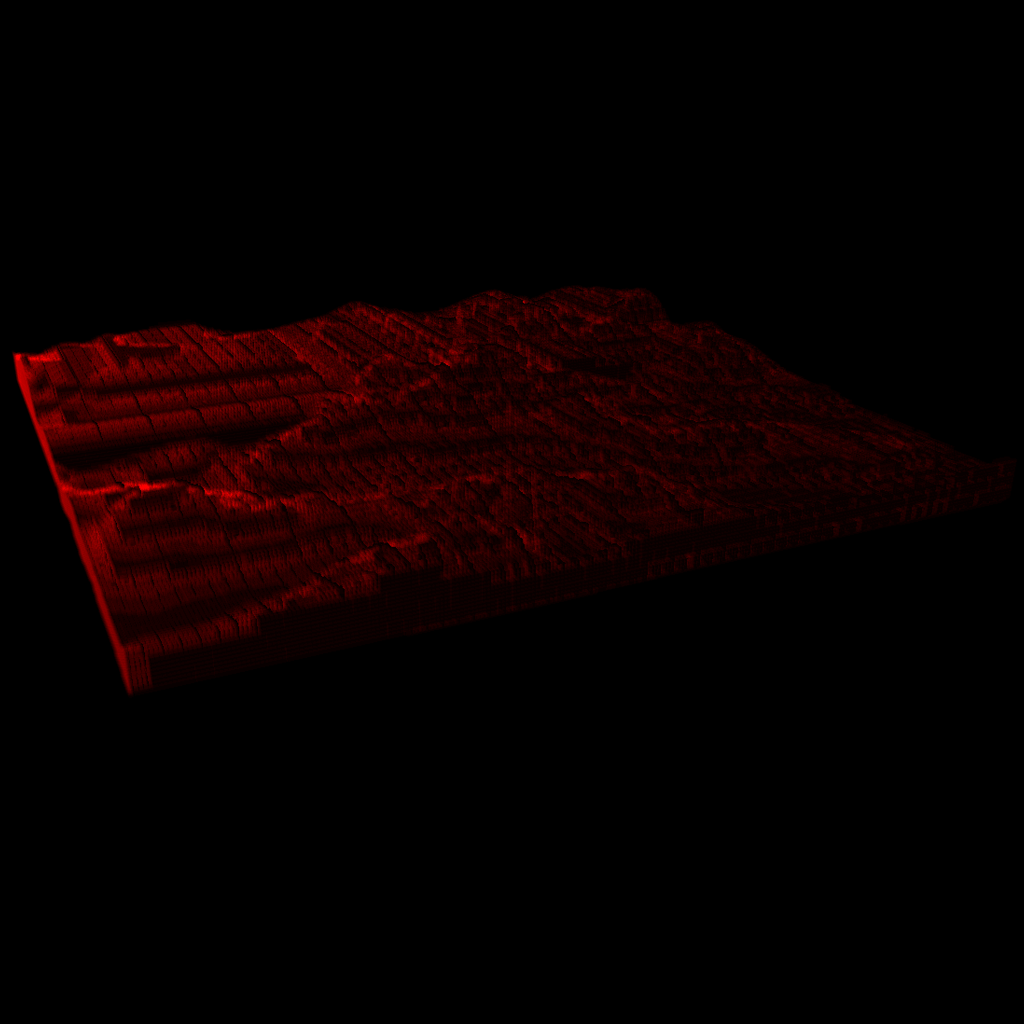
\includegraphics[height=100px]{images/graphics/overdraw-terrain2-pmoc.png}
    \caption{}
    \parbox{\linewidth}{\centering\footnotesize Per-Meshlet\\Occlusion Culling}
  \end{subfigure}
  \begin{subfigure}{100px}
    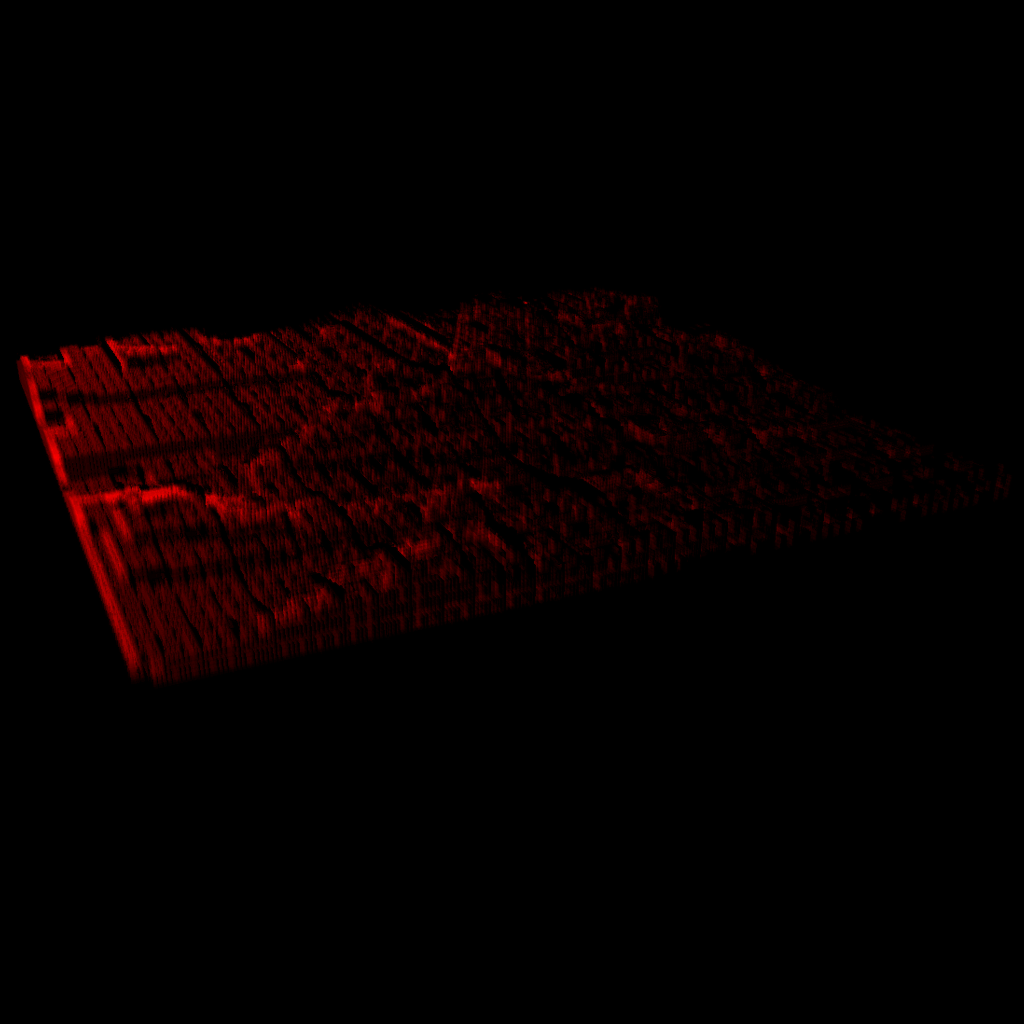
\includegraphics[height=100px]{images/graphics/overdraw-terrain2-diff.png}
    \caption{}
    \parbox{\linewidth}{\centering\footnotesize Difference\\(b) vs. (c)}
  \end{subfigure}

  \caption{Overdraw of the pixels from two different camera angles. 
  The image values are enhanced for better visualization.}
  \label{fig:terrain-overdraw}
\end{figure}


\noindent
As shown in Figure \ref{fig:terrain-overdraw}, the \ac{PONOC} configuration clearly 
featured more overdraw than the comparison configuration. In the first row, it is evident that 
the left lower corner features a lot of overdraw, which was decreased by switching to the 
\ac{PMOC} configuration. The maximum draws per pixel were 86 and 45, respectively, in 
favor of the \ac{PMOC}. Without culling, the overdraw was 298 draws per pixel.

\clearpage



\subsection*{Hairball}

For low resolutions, the \emph{Hairball} is an inherently complex scene to render. It features a lot 
of tiny details, which were assumed to be not sufficient in density to completely fill octree nodes, 
resulting in an unfavorable data layout to test the limits of the occlusion culling algorithm.

\subsubsection*{Culling Results} \label{subsubsec-culling-results-hairball}

% -------------------------------------- HAIRBALL 256 -------------------------------------

\begin{figure}[!htb]              % Hairball 256 Voxels Test Anim
    \begin{center}
      \begin{tikzpicture}
        \begin{axis}[
            width=\linewidth, % Scale the plot to \linewidth
            height=100px,
            xlabel={Frames},
            ylabel={Visible Voxels},
            grid,
            xmin=0,
            xmax=940,
            ymin=450000,
            ymax=800000,
            legend style={at={(0.5,1.7)}, anchor=north, legend columns=2},
          ]
          \addplot[blue, no marks, solid] table[col sep=comma, x=frame, x expr=\thisrow{frame} * 940 / 940, y=visible_voxels]{./plotdata/hairball_256_voxels.csv};
          \addplot[red, no marks, solid] table[col sep=comma, x=frame, x expr=\thisrow{frame} * 940 / 1187, y=visible_voxels]{./plotdata/hairball_256_voxels_pmoc.csv};
          \addplot[blue, dotted, no marks, domain=0:940, samples=50] {697549};
          \addplot[red, dotted, no marks, domain=0:940, samples=50] {581663};
          \legend{Per-Octree Occlsion Culling, Per-Meshlet Occlusion Culling}
        \end{axis}
      \end{tikzpicture}

      \begin{tikzpicture}
        \begin{axis}[
            width=\linewidth, % Scale the plot to \linewidth
            height=100px,
            xlabel={Frames},
            ylabel={Computed Nodes},
            grid,
            xmin=0,
            xmax=940,
            ymin=15000,
            ymax=25000,
            legend style={at={(0.5,1.7)}, anchor=north, legend columns=2},
          ]
          \addplot[blue, no marks, solid] table[col sep=comma, x=frame, x expr=\thisrow{frame} * 940 / 940, y=visible_nodes]{./plotdata/hairball_256_nodes.csv};
          \addplot[red, no marks, solid] table[col sep=comma, x=frame, x expr=\thisrow{frame} * 940 / 1187, y=visible_nodes]{./plotdata/hairball_256_nodes_pmoc.csv};
          \addplot[blue, dotted, no marks, domain=0:940, samples=50] {21229};
          \addplot[red, dotted, no marks, domain=0:940, samples=50] {18925};
          \legend{Per-Octree Occlsion Culling, Per-Meshlet Occlusion Culling}
        \end{axis}
      \end{tikzpicture}

      \caption{\textbf{First:} The amount of visible voxels over the course of the test animation. \\
      \textbf{Second:} The amount of visible octree nodes over the course of the test animation.}
      \label{plt:hairball-256-culling-res-voxels}
    \end{center}
  \end{figure}

% ----------------------------------------------------------------------------------------

\noindent
Figure \ref{plt:hairball-256-culling-res-voxels} shows the amount of culled voxels and octree nodes 
over the course of the test animation for both occlusion culling configurations. The \emph{Hairball} 
scene showed a drastic drop in visible voxels when it was viewed from above instead of from the side. 
This suggests that the scene is highly dependent on the camera position and angle. \\

\noindent
The average number of visible voxels was 697,549 for \ac{PONOC} and 581,663 for \ac{PMOC}, while the 
number of total voxels in the scene was 1,652,435. The average amount of visible octree nodes was 
21,229 for \ac{PONOC} and 18,925 for \ac{PMOC}. The number of total octree nodes in the scene was 
39,591. \\

\noindent
The data suggests that the \emph{Hairball} was able to be used for both occlusion culling configurations 
and benefitted from the more granular \ac{PMOC} while still being considerably dependent on the viewing 
angle of the camera. The average culling ratio was $57.8\%$ for \ac{PONOC} and $64.8\%$ for \ac{PMOC}. 
For the former, the number of visible voxels diverged by a maximum of $12.91\%$ from the average value, 
while the latter diverged by a maximum of $14.29\%$. For the visible octree nodes, the variations were 
$12.98\%$ for \ac{PONOC} and $13.78\%$ for \ac{PMOC}. These values show that the occlusion culling 
algorithm wasn't able to cull significantly more voxels for a given camera angle than from any other 
camera angle in the scene. 

\subsubsection*{CPU Performance Results} \label{subsubsec-cpu-performance-results-hairball}

\begin{figure}[!htbp]              % Hairball CPU times
  \begin{center}
    \begin{tikzpicture}
      \begin{axis}[
          width=\linewidth,
          height=100px,
          xlabel={Frames},
          ylabel={Update Time (s)},
          grid,
          xmin=0,
          xmax=940,
          ymin=0,
          ymax=0.00005,
          legend style={at={(0.5,1.8)}, anchor=north, legend columns=2},
        ]
        \addplot[brown!60, no marks, solid] table[col sep=comma, x=frame, x expr=\thisrow{frame} * 940 / 1301, y=time]{./plotdata/cpu/hairball_256_updateTime_nocull.csv};
        \addplot[blue, no marks, solid] table[col sep=comma, x=frame, x expr=\thisrow{frame} * 940 / 1421, y=time]{./plotdata/cpu/hairball_256_updateTime_pooc.csv};
        \addplot[red, no marks, solid] table[col sep=comma, x=frame, x expr=\thisrow{frame} * 940 / 1446, y=time]{./plotdata/cpu/hairball_256_updateTime.csv};
        \legend{No Occlusion Culling, Per-Octree Occlsion Culling, Per-Meshlet Occlusion Culling}
      \end{axis}
    \end{tikzpicture}
    \begin{tikzpicture}
      \begin{axis}[
          width=\linewidth,
          height=100px,
          xlabel={Frames},
          ylabel={Render Time (s)},
          grid,
          xmin=0,
          xmax=940,
          ymin=0,
          ymax=0.00025,
          legend style={at={(0.5,1.8)}, anchor=north, legend columns=2},
        ]
        \addplot[brown!60, no marks, solid] table[col sep=comma, x=frame, x expr=\thisrow{frame} * 940 / 1301, y=time]{./plotdata/cpu/hairball_256_renderTime_nocull.csv};
        \addplot[blue, no marks, solid] table[col sep=comma, x=frame, x expr=\thisrow{frame} * 940 / 1421, y=time]{./plotdata/cpu/hairball_256_renderTime_pooc.csv};
        \addplot[red, no marks, solid] table[col sep=comma, x=frame, x expr=\thisrow{frame} * 940 / 1446, y=time]{./plotdata/cpu/hairball_256_renderTime.csv};
        \legend{No Occlusion Culling, Per-Octree Occlsion Culling, Per-Meshlet Occlusion Culling}
      \end{axis}
    \end{tikzpicture}
  \end{center}
  \caption{Overview of the render times over the course of the test animation. The upper graph shows the time 
  each frame took to execute the \emph{Update()} function on the \ac{CPU}. The lower graph shows the time each 
  frame took to execute the function \emph{Render()} on the \ac{CPU}. This includes the completion of the 
  \ac{GPU} computations.}
  \label{plt:hairball-256-culling-cpu-time}
\end{figure}

\noindent
Figure \ref{plt:hairball-256-culling-cpu-time} shows the \ac{CPU} times during the test animation. During 
the first 200 frames of the test animation, a difference is visible between the base pipeline without 
occlusion culling and the two occlusion culling configurations. This difference is visible in both the 
\emph{Update()} and the \emph{Render()} function frame time graphs. Neither variation could be attributed 
to any pipeline characteristic and was therefore considered to be of no significance for the evaluation of 
the occlusion culling algorithm.

\subsubsection*{GPU Performance Results} \label{subsubsec-gpu-performance-results-hairball}

Figure \ref{fig:hairball-gpu-times} shows the \ac{GPU} timings for all tested pipeline configurations.
The \emph{Hairball} scene showed a significant difference between the base pipeline and the two occlusion 
culling configurations. The \ac{PONOC} configuration was able to decrease the \ac{GPU} time by $54.4\%$ 
as compared to the base pipeline. The \ac{PMOC} configuration was able to optimize \ac{GPU} times by 
$61.2\%$ compared to the base pipeline. In this case, the \ac{PMOC} didn't perform tremendously better 
than the \ac{PONOC} configuration. Nevertheless, depending on the camera angle, both culling configurations 
could successfully increase the \ac{GPU} performance. \\

\noindent
When comparing the average values, the depth prepass diverged by only 0.75 microseconds in favor of the \ac{PMOC}.  

\begin{figure}[!htb]
  \centering
  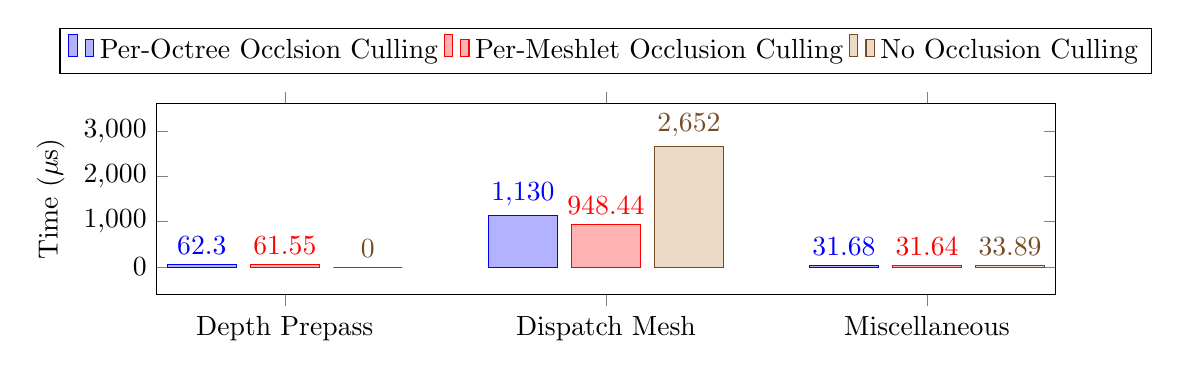
\begin{tikzpicture}
    \begin{axis}[
        height=4cm,
        width=13cm,
        x tick label style={/pgf/number format/1000 sep=},
        ylabel={Time ($\mu$s)},
        legend style={at={(0.5,1.4)}, anchor=north, legend columns=-1},
        symbolic x coords={DepthPrepass, DispatchMesh, Misc},
        xticklabels={Depth Prepass, Dispatch Mesh, Miscellaneous},
        xtick=data,
        ybar=0.4,
        bar width=25pt,
        ymin=0,
        ymax=3000,
        nodes near coords,
        enlargelimits=0.2,
    ]
    \addplot+[bar shift=-30pt] coordinates {(DepthPrepass,62.30) (DispatchMesh,1130.00) (Misc,31.68)};
    \addplot+[bar shift=0pt] coordinates {(DepthPrepass,61.55) (DispatchMesh,948.44) (Misc,31.6354)};
    \addplot+[bar shift=30pt] coordinates {(DepthPrepass,0) (DispatchMesh,2652.00) (Misc,33.8856)};
    \legend{Per-Octree Occlsion Culling, Per-Meshlet Occlusion Culling, No Occlusion Culling}
    \end{axis}
  \end{tikzpicture}

  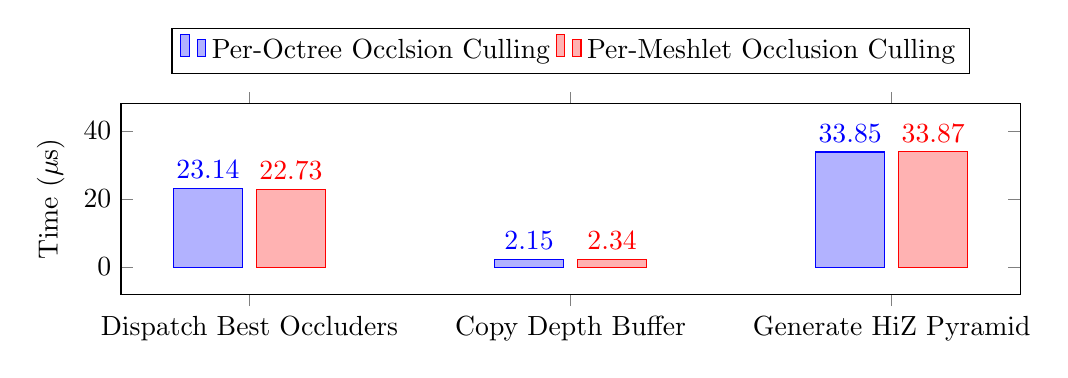
\begin{tikzpicture}
    \begin{axis}[
        height=4cm,
        width=13cm,
        x tick label style={/pgf/number format/1000 sep=},
        ylabel={Time ($\mu$s)},
        legend style={at={(0.5,1.4)}, anchor=north, legend columns=-1},
        symbolic x coords={DispatchBestOccluders, CopyTex, GenMipChain},
        xticklabels={Dispatch Best Occluders, Copy Depth Buffer, Generate \ac{HiZ} Pyramid},
        xtick=data,
        ybar=0.4,
        bar width=25pt,
        ymin=0,
        ymax=40,
        nodes near coords,
        enlargelimits=0.2,
    ]
    \addplot+[bar shift=-15pt] coordinates {(DispatchBestOccluders,23.14) (CopyTex,2.15) (GenMipChain,33.85)};
    \addplot+[bar shift=15pt] coordinates {(DispatchBestOccluders,22.73) (CopyTex,2.34) (GenMipChain,33.87)};
    \legend{Per-Octree Occlsion Culling, Per-Meshlet Occlusion Culling}
    \end{axis}
  \end{tikzpicture}
  \caption{\textbf{First:} The complete time measured on the \ac{GPU}. The \emph{Depth Prepass} is the extra 
  overhead introduced by the \ac{HZB}. The \emph{Dispatch Mesh} is the drawing of the meshes, including the 
  occlusion culling. \emph{Miscellaneous} includes a small amount of \emph{Barriers} used for synchronization 
  and the rendering of some debug \ac{UI}. It is considered to be more or less static in computation time and 
  is not part of the actual algorithm measured in this experiment. \textbf{Second:} The time measured in the 
  \emph{Depth Prepass}. The \emph{Dispatch Best Occluders} is the drawing to the depth buffer. The 
  \emph{Copy Depth Buffer} computation copies the depth buffers content into the final \ac{HiZ} resource. 
  Finally, \emph{Generate HiZ Pyramid} shows the \ac{HiZ} creation, which is done sequentially.}
  \label{fig:hairball-gpu-times}
\end{figure}

\subsubsection*{Overdraw}

\begin{figure}[!htb]
  \centering  
  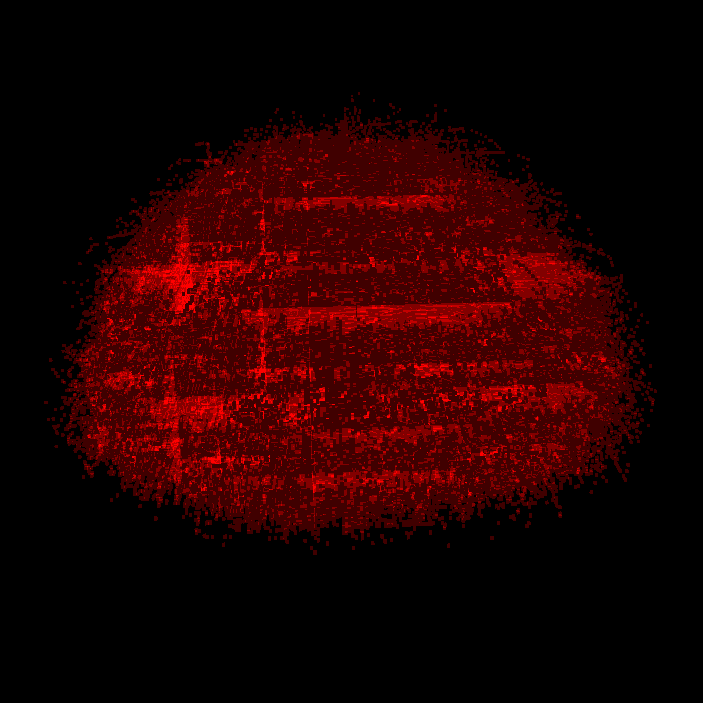
\includegraphics[height=100px]{images/graphics/overdraw-hairball1-nocull.png}
  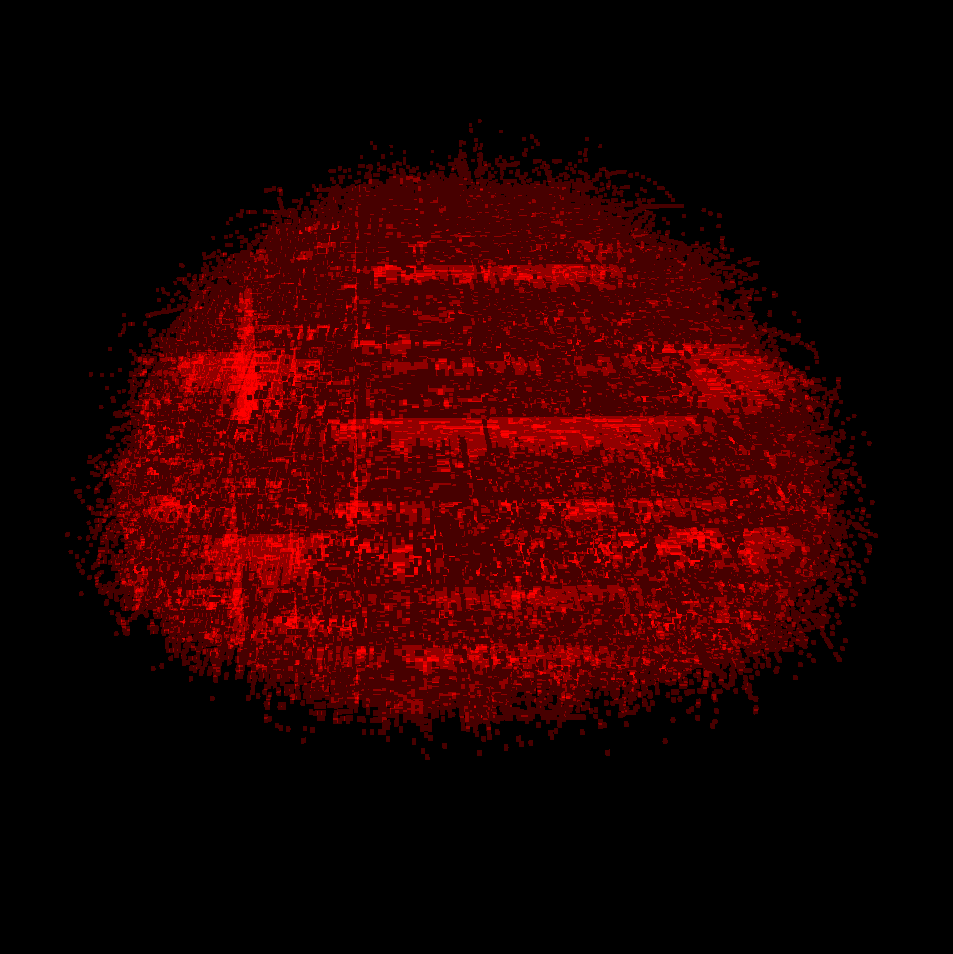
\includegraphics[height=100px]{images/graphics/overdraw-hairball1-pooc.png}
  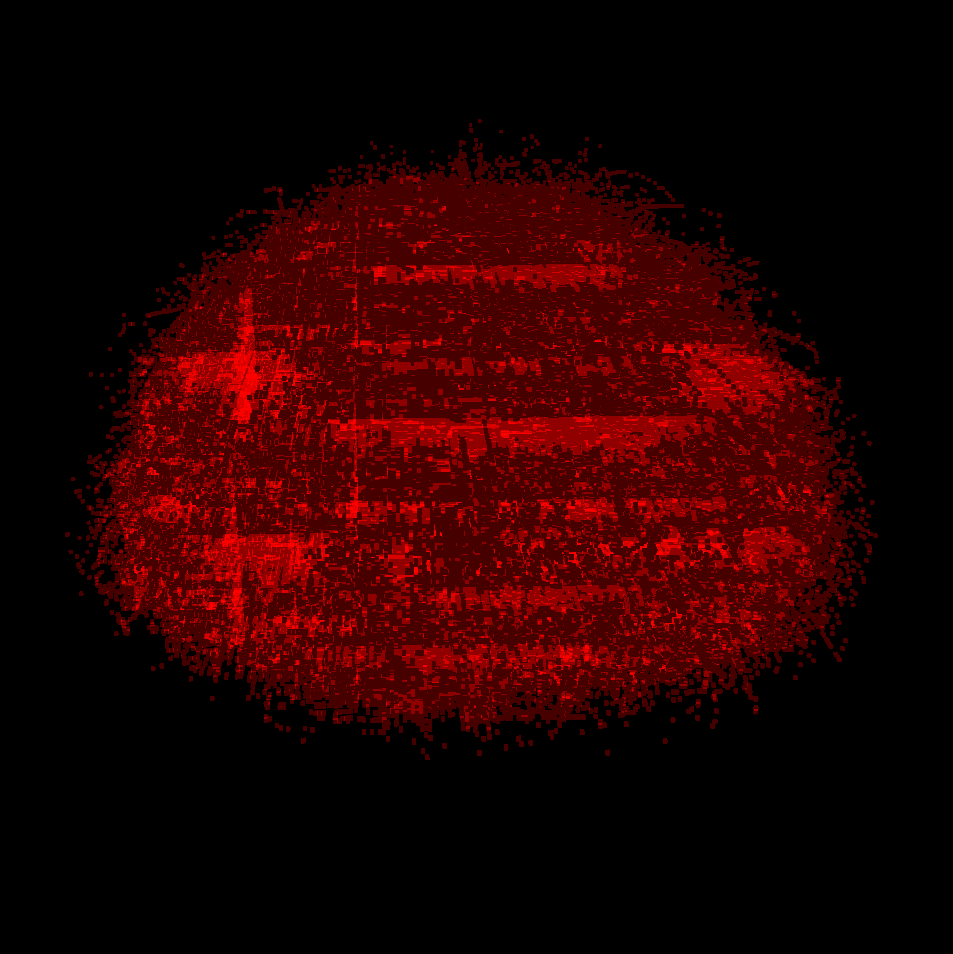
\includegraphics[height=100px]{images/graphics/overdraw-hairball1-pmoc.png}
  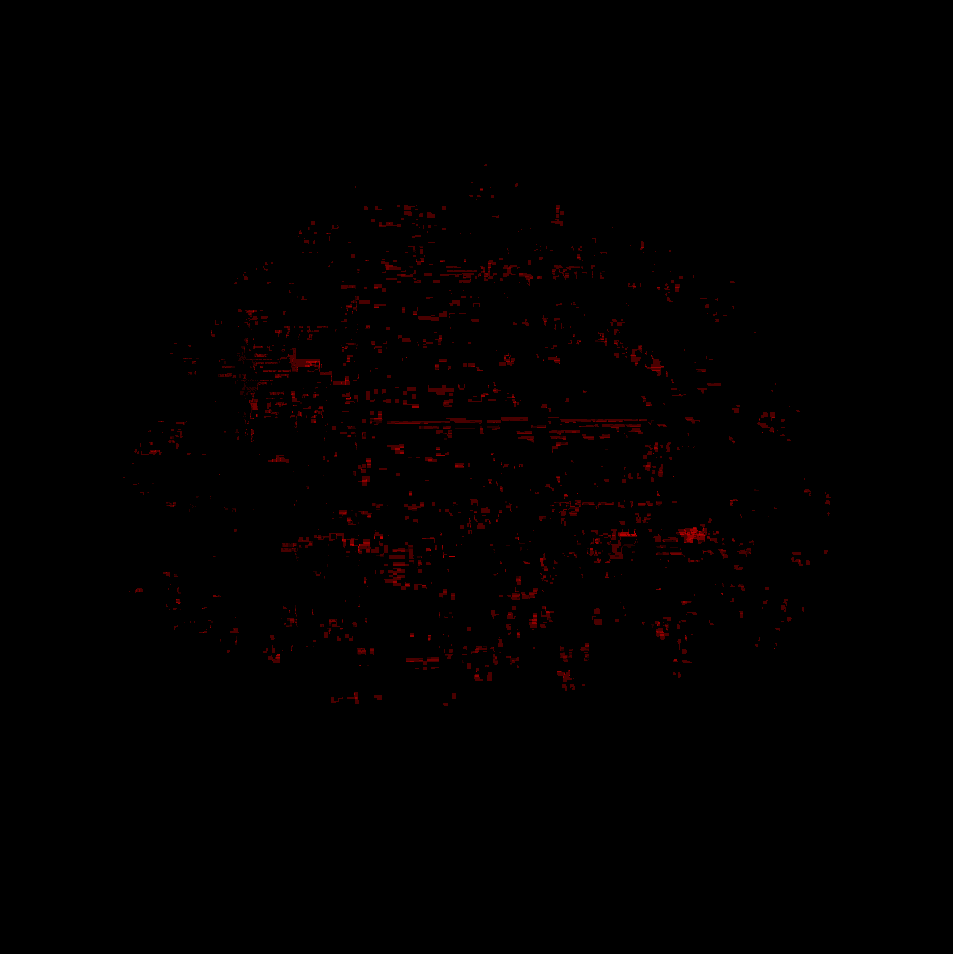
\includegraphics[height=100px]{images/graphics/overdraw-hairball1-diff.png}

  \begin{subfigure}{100px}
    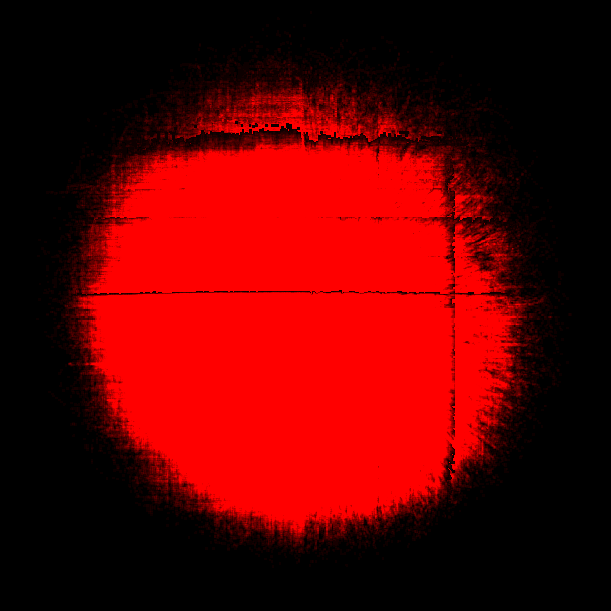
\includegraphics[height=100px]{images/graphics/overdraw-hairball2-nocull.png}
    \caption{}
    \parbox{\linewidth}{\centering\footnotesize No Occlusion\\Culling}
  \end{subfigure}
  \begin{subfigure}{100px}
    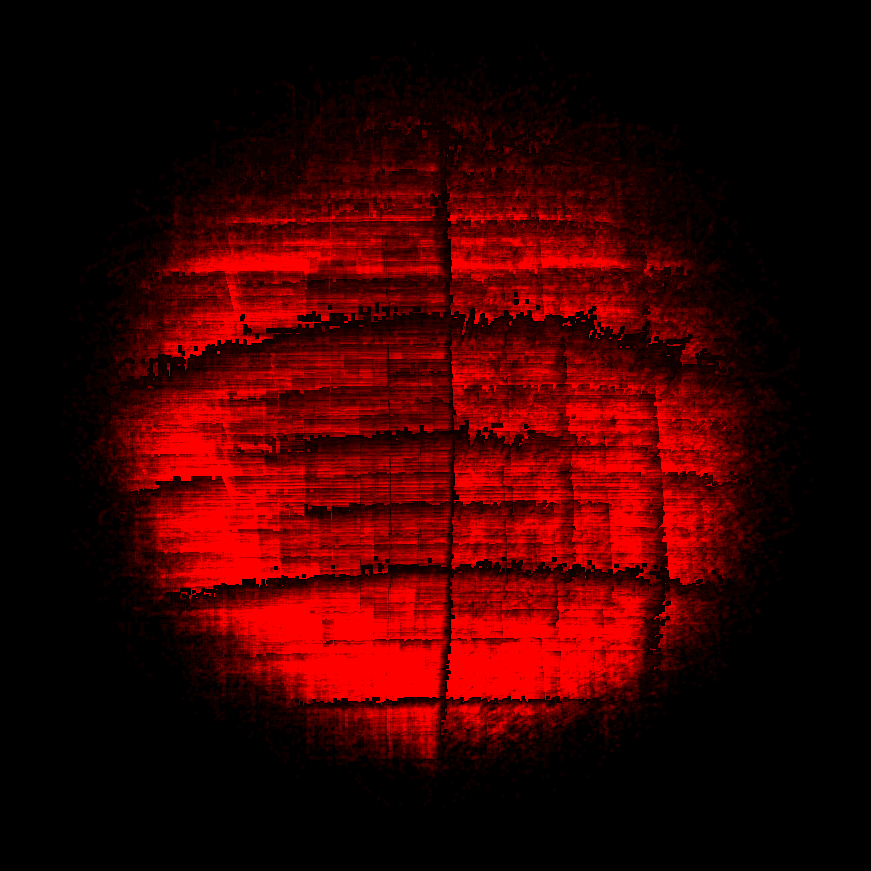
\includegraphics[height=100px]{images/graphics/overdraw-hairball2-pooc.png}
    \caption{}
    \parbox{\linewidth}{\centering\footnotesize Per-Octree Node\\Occlusion Culling}
  \end{subfigure}
  \begin{subfigure}{100px}
    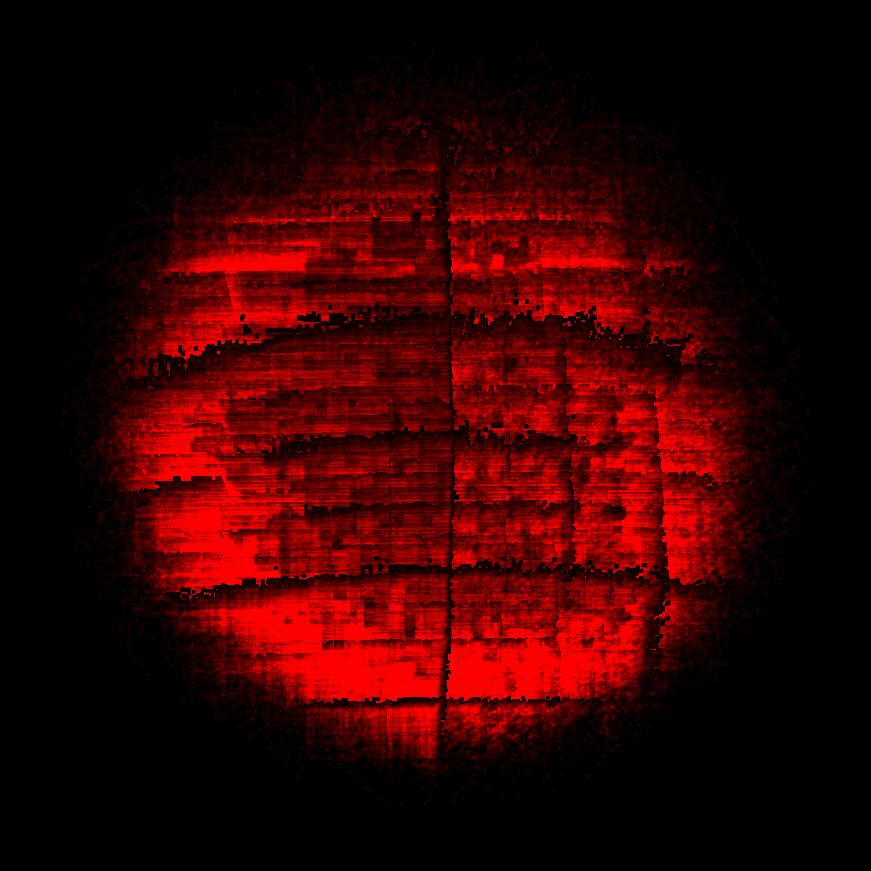
\includegraphics[height=100px]{images/graphics/overdraw-hairball2-pmoc.png}
    \caption{}
    \parbox{\linewidth}{\centering\footnotesize Per-Meshlet\\Occlusion Culling}
  \end{subfigure}
  \begin{subfigure}{100px}
    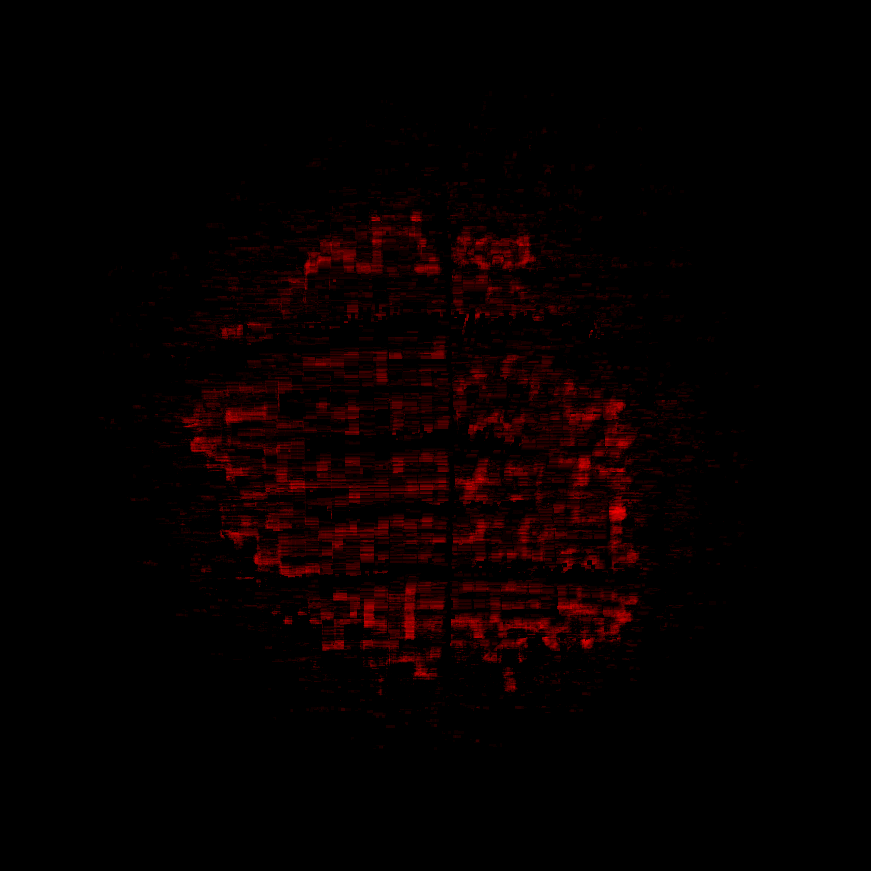
\includegraphics[height=100px]{images/graphics/overdraw-hairball2-diff.png}
    \caption{}
    \parbox{\linewidth}{\centering\footnotesize Difference\\(b) vs. (c)}
  \end{subfigure}

  \caption{Overdraw of the pixels from two different camera angles. 
  The image values are enhanced for better visualization.}
  \label{fig:hairball-overdraw}
\end{figure}

\noindent
Figure \ref{fig:hairball-overdraw} shows that the overdraw was similar for both configurations, 
but still in favor of \ac{PMOC}. The last column, featuring the difference values between both 
configurations, shows this particularly well. There is only a small difference between the  
measurements, which is also reflected in the maximum amount of overdraw. The \ac{PONOC} resulted 
in a maximum of 54 draws to one pixel, and the \ac{PMOC} configuration resulted in a maximum of 
51 draws. Without occlusion culling, the overdraw reached its maximum at 117 draws to one pixel.

\clearpage


\subsection*{Cross-Comparison}

Now that each model has been analyzed individually, the data is cross-compared over all models to 
discuss the overall results the measurements provided. Table \ref{tbl:culling-result-overview} shows 
an overview of all models and some of the most meaningful data points. 
  
\begin{table}[!htb]
  \begin{tabular}{|lccccc|}
    \hline
    \multicolumn{1}{|l|}{}                          & \multicolumn{1}{|c|}{\textbf{Stanford Lucy}}  & \multicolumn{1}{c|}{\textbf{Stanford Bunny}}  & \multicolumn{1}{c|}{\textbf{Torus}}   & \multicolumn{1}{c|}{\textbf{Terrain}}     & \multicolumn{1}{c|}{\textbf{Hairball}}    \\ \hline
    \multicolumn{1}{|l|}{Best Occluder Count}       & \multicolumn{1}{c|}{1600}                     & \multicolumn{1}{c|}{8256}                     & \multicolumn{1}{c|}{7168}             & \multicolumn{1}{c|}{6976}                 & \multicolumn{1}{c|}{5056}                 \\ 
    \multicolumn{1}{|l|}{Total Voxel Count}         & \multicolumn{1}{c|}{331,254}                  & \multicolumn{1}{c|}{3,379,738}                & \multicolumn{1}{c|}{2,311,006}        & \multicolumn{1}{c|}{953,362}              & \multicolumn{1}{c|}{1,652,435}            \\
    \multicolumn{1}{|l|}{Total Octree Nodes}        & \multicolumn{1}{c|}{6,830}                    & \multicolumn{1}{c|}{57,481}                   & \multicolumn{1}{c|}{39,794}           & \multicolumn{1}{c|}{18,465}               & \multicolumn{1}{c|}{39,591}               \\
    \multicolumn{1}{|l|}{Avg. Node Population}      & \multicolumn{1}{c|}{\textbf{48.5 \%}}         & \multicolumn{1}{c|}{\textbf{91.9 \%}}         & \multicolumn{1}{c|}{\textbf{90.7 \%}} & \multicolumn{1}{c|}{\textbf{80.7 \%}}     & \multicolumn{1}{c|}{\textbf{65.2 \%}}     \\ \hline
    \multicolumn{6}{|c|}{\textbf{Scene Resolution: $256^3$ - Per-Octree Occlusion Culling}}                                                                                                                                                                                         \\ \hline
    \multicolumn{1}{|l|}{Avg. Visible Voxels}       & \multicolumn{1}{c|}{140,842}                  & \multicolumn{1}{c|}{385,210}                  & \multicolumn{1}{c|}{359,313}          & \multicolumn{1}{c|}{396,228}              & \multicolumn{1}{c|}{697,549}              \\
    \multicolumn{1}{|l|}{Avg. Culled Voxels}        & \multicolumn{1}{c|}{190,412}                  & \multicolumn{1}{c|}{2,994,528}                & \multicolumn{1}{c|}{1,951,693}        & \multicolumn{1}{c|}{557,134}              & \multicolumn{1}{c|}{954,886}              \\
    \multicolumn{1}{|l|}{Avg. Culled Voxel Ratio}   & \multicolumn{1}{c|}{\textbf{57.5 \%}}         & \multicolumn{1}{c|}{\textbf{88.6 \%}}         & \multicolumn{1}{c|}{\textbf{84.5 \%}} & \multicolumn{1}{c|}{\textbf{58.4 \%}}     & \multicolumn{1}{c|}{\textbf{57.8 \%}}     \\ \hline
    \multicolumn{1}{|l|}{Avg. Visible Nodes}        & \multicolumn{1}{c|}{3,460}                    & \multicolumn{1}{c|}{8,519}                    & \multicolumn{1}{c|}{7,712}            & \multicolumn{1}{c|}{8,207}                & \multicolumn{1}{c|}{21,229}               \\
    \multicolumn{1}{|l|}{Avg. Culled Nodes}         & \multicolumn{1}{c|}{3,370}                    & \multicolumn{1}{c|}{48,962}                   & \multicolumn{1}{c|}{32,082}           & \multicolumn{1}{c|}{10,258}               & \multicolumn{1}{c|}{18,362}               \\
    \multicolumn{1}{|l|}{Avg. Culled Node Ratio}    & \multicolumn{1}{c|}{\textbf{49.3 \%}}         & \multicolumn{1}{c|}{\textbf{85.2 \%}}         & \multicolumn{1}{c|}{\textbf{80.6 \%}} & \multicolumn{1}{c|}{\textbf{55.6 \%}}     & \multicolumn{1}{c|}{\textbf{46.4 \%}}     \\ \hline
    \multicolumn{6}{|c|}{\textbf{Scene Resolution: $256^3$ - Per-Meshlet Occlusion Culling}}                                                                                                                                                                                        \\ \hline
    \multicolumn{1}{|l|}{Avg. Visible Voxels}       & \multicolumn{1}{c|}{84,082}                   & \multicolumn{1}{c|}{180,266}                  & \multicolumn{1}{c|}{170,772}          & \multicolumn{1}{c|}{180,440}              & \multicolumn{1}{c|}{581,663}              \\
    \multicolumn{1}{|l|}{Avg. Culled Voxels}        & \multicolumn{1}{c|}{247,226}                  & \multicolumn{1}{c|}{3,199,472}                & \multicolumn{1}{c|}{2,140,234}        & \multicolumn{1}{c|}{772,922}              & \multicolumn{1}{c|}{1,070,722}            \\
    \multicolumn{1}{|l|}{Avg. Culled Voxel Ratio}   & \multicolumn{1}{c|}{\textbf{74.6 \%}}         & \multicolumn{1}{c|}{\textbf{94.7 \%}}         & \multicolumn{1}{c|}{\textbf{92.6 \%}} & \multicolumn{1}{c|}{\textbf{81.1 \%}}     & \multicolumn{1}{c|}{\textbf{64.8 \%}}     \\ \hline
    \multicolumn{1}{|l|}{Avg. Visible Nodes}        & \multicolumn{1}{c|}{2,483}                    & \multicolumn{1}{c|}{5,415}                    & \multicolumn{1}{c|}{4,768}            & \multicolumn{1}{c|}{3,832}                & \multicolumn{1}{c|}{18,925}               \\
    \multicolumn{1}{|l|}{Avg. Culled Nodes}         & \multicolumn{1}{c|}{4,347}                    & \multicolumn{1}{c|}{52,066}                   & \multicolumn{1}{c|}{35,026}           & \multicolumn{1}{c|}{14,633}               & \multicolumn{1}{c|}{20,666}               \\
    \multicolumn{1}{|l|}{Avg. Culled Node Ratio}    & \multicolumn{1}{c|}{\textbf{63.6 \%}}         & \multicolumn{1}{c|}{\textbf{90.6 \%}}         & \multicolumn{1}{c|}{\textbf{88.0 \%}} & \multicolumn{1}{c|}{\textbf{79.2 \%}}     & \multicolumn{1}{c|}{\textbf{52.2 \%}}     \\ \hline
    
  \end{tabular}
  \caption{An overview comparing the most significant measures for all models. 
  The first part of the table shows general model specific data. The second part shows results for the 
  \ac{PONOC} configuration and the last part shows results for the \ac{PMOC} configuration.}
  \label{tbl:culling-result-overview}
\end{table}
  
\noindent
The table shows the average culling data for all models. The row \emph{Average Node Population} is 
particularly interesting as it shows how the culling results related to the degree to which the octree 
nodes were filled. The higher this value, the more the octree nodes were filled on average. A high 
average fill indicates the existence of a lot of best occluders relative to the amount of voxels and 
octree nodes present in the scene. This measure strongly correlates with the average ratio of culled 
voxels and octree nodes. \\

\noindent
The table shows all aspects of the \ac{PONOC} and \ac{PMOC} configurations. It demonstrates that the 
occlusion culling algorithm was able to cull a greater amount of voxels when using the \ac{PMOC} 
configuration. Additionally, across all models, a higher amount of best occluders consequently 
resulted in a higher culling ratio. \\

\begin{figure}[!htb]
  \centering
  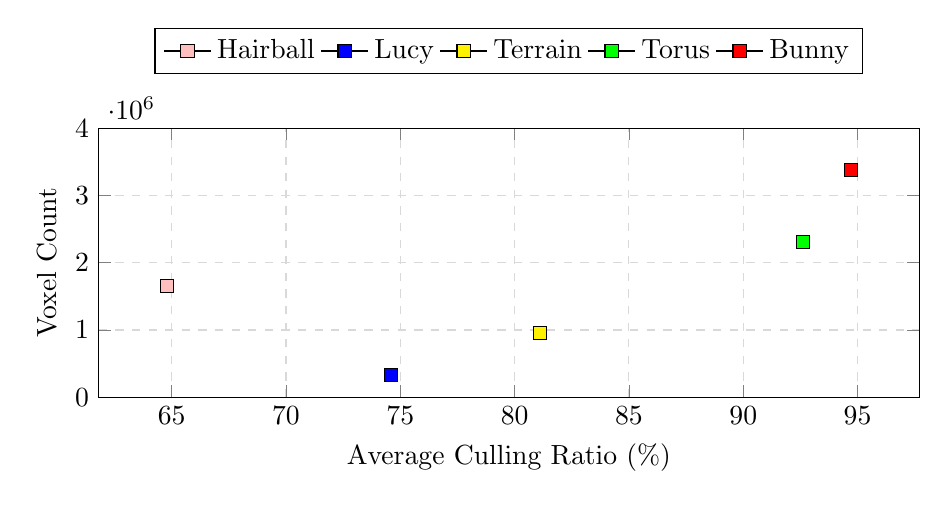
\begin{tikzpicture}
      \begin{axis}[
          width=12cm,
          height=5cm,
          ylabel={Voxel Count},
          xlabel={Average Culling Ratio (\%)},
          grid=major,
          grid style={dashed, gray!30},
          legend style={at={(0.5,1.2)}, anchor=south, legend columns=5},
          ymin=0, ymax=4000000,
          scaled x ticks=false,
          ]
      
          \addplot[mark=square*, mark options={scale=1.2, fill=pink},] coordinates  {(64.8, 1652435)};
          \addplot[mark=square*, mark options={scale=1.2, fill=blue},] coordinates {(74.6, 331254)};
          \addplot[mark=square*, mark options={scale=1.2, fill=yellow},] coordinates {(81.1, 953362)};
          \addplot[mark=square*, mark options={scale=1.2, fill=green},] coordinates {(92.6, 2311006)};
          \addplot[mark=square*, mark options={scale=1.2, fill=red},] coordinates {(94.7, 3379738)};
          \legend{Hairball, Lucy, Terrain, Torus, Bunny}
      \end{axis}
  \end{tikzpicture}

  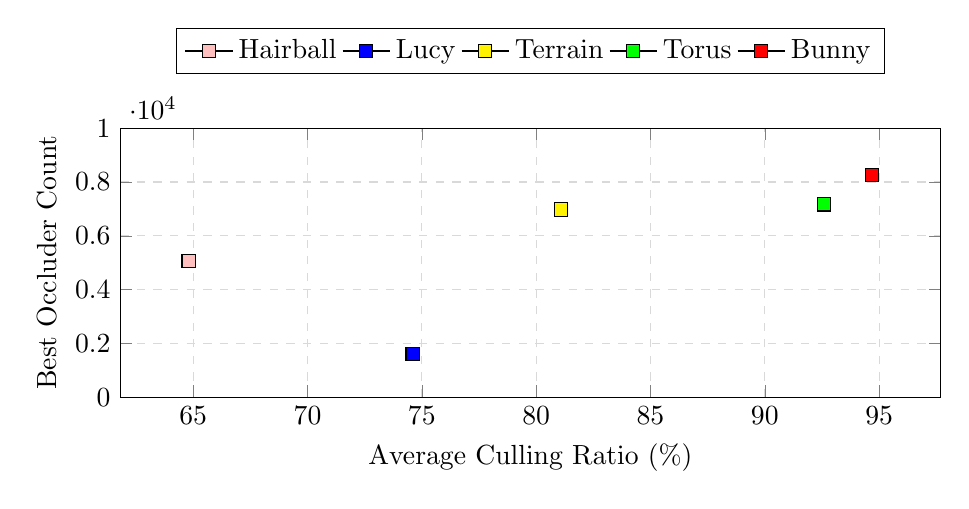
\begin{tikzpicture}
      \begin{axis}[
          width=12cm,
          height=5cm,
          ylabel={Best Occluder Count},
          xlabel={Average Culling Ratio (\%)},
          grid=major,
          grid style={dashed, gray!30},
          legend style={at={(0.5,1.2)}, anchor=south, legend columns=5},
          ymin=0, ymax=10000,
          scaled x ticks=false,
          ]

          \addplot[mark=square*, mark options={scale=1.2, fill=pink},] coordinates  {(64.8, 5056)};
          \addplot[mark=square*, mark options={scale=1.2, fill=blue},] coordinates {(74.6, 1600)};
          \addplot[mark=square*, mark options={scale=1.2, fill=yellow},] coordinates {(81.1, 6976)};
          \addplot[mark=square*, mark options={scale=1.2, fill=green},] coordinates {(92.6, 7168)};
          \addplot[mark=square*, mark options={scale=1.2, fill=red},] coordinates {(94.7, 8256)};
          \legend{Hairball, Lucy, Terrain, Torus, Bunny}
      \end{axis}
  \end{tikzpicture}
  \caption{Upper: The relation between voxel count and culling ratio. \\
  Lower: The relation between best occluder count and culling ratio.}
  \label{plt:culling-efficiency-voxel-node-count}
\end{figure}

\noindent
Figure \ref{plt:culling-efficiency-voxel-node-count} outlines the relationship between the voxel 
count and the culling ratio compared to the relation between the best occluder count and the culling 
ratio. The data shows a correlation between the culling ratio and the voxel count, or best occluder 
count, respectively. It also shows that this correlation only remained as long as the scene topology 
was sufficiently suitable for the occlusion culling algorithm. The complex \emph{Hairball} scene 
demonstrates how unfavorable topology led to a drop in culling ratio. This is additionally confirmed 
by the \emph{Terrain} and \emph{Torus} scenes, which featured a similar amount of best occluders 
but showed significantly different average culling ratios. Ultimately, the culling ratio depended 
on topology, voxel and best occluder counts, and model size. \\


\begin{figure}[!htb]    % GPU time overview
  \begin{center}
    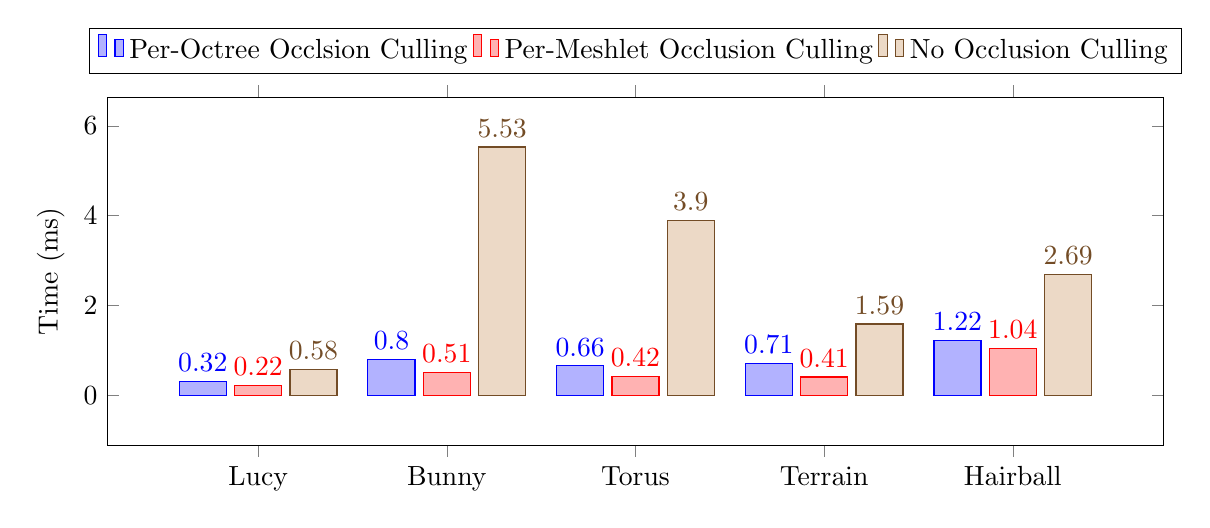
\begin{tikzpicture}
      \begin{axis}[
          height=6cm,
          width=15cm,
          x tick label style={/pgf/number format/1000 sep=},
          ylabel={Time (ms)},
          legend style={at={(0.5,1.2)}, anchor=north, legend columns=-1},
          symbolic x coords={Lucy, Bunny, Torus, Terrain, Hairball},
          xtick=data,
          ybar=0.4,
          bar width=17pt,
          ymin=0,
          nodes near coords,
          enlargelimits=0.2,
      ]
      \addplot+[bar shift=-20pt] coordinates {(Lucy,0.32) (Bunny,0.80) (Torus,0.66) (Terrain,0.71) (Hairball,1.22)};
      \addplot+[bar shift=0pt] coordinates {(Lucy,0.22) (Bunny,0.51) (Torus,0.42) (Terrain,0.41) (Hairball,1.04)};
      \addplot+[bar shift=20pt] coordinates {(Lucy,0.58) (Bunny,5.53) (Torus,3.90) (Terrain,1.59) (Hairball,2.69)};
      \legend{Per-Octree Occlsion Culling, Per-Meshlet Occlusion Culling, No Occlusion Culling}
      \end{axis}
    \end{tikzpicture}
  \end{center}
  \caption{An overview of the average \ac{GPU} timings for all tested models.}
  \label{fig:gpu-performance-overview}
\end{figure}

\noindent
The measurements indicate that the \ac{GPU} performance significantly benefitted from the occlusion 
culling throughout all scenes. Figure \ref{fig:gpu-performance-overview} shows an overview of all 
scenes comparing the time spent on the \ac{GPU} for both tested configurations. The \ac{CPU} 
performance did not show any significant differences that could reliably be traced back to the 
tested approaches. Small differences were usually in the order of about 1-10 microseconds and could 
not be reliably attributed to either of the two culling configurations. \\

\noindent
The individual overdraw measurements suggest that the amount of overdraw significantly varied with the 
change of the camera angle. It is evident that the overdraw could be reduced best using models with high 
volumes and avoiding small and thin details. In general, the \ac{PMOC} approach was able to achieve 
better results in terms of overdraw, although it was highly dependent on camera angle and dense best 
occluder coverage. Usually, outer edges of models with curved surfaces could not be covered very well 
because of the lack of best occluders. \\
